\documentclass[
a5paper,
%paper=5.5in:8.5in,
BCOR=7mm,
twoside,
DIV=calc,
11pt,
usegeometry,
headings=big]{scrbook} % Document font size and paper size

\usepackage{graphicx}
\usepackage{verse}
\usepackage{xcolor}
\usepackage{fontspec}
\usepackage[T1]{fontenc} % International character encodings
\usepackage{makeidx}
\usepackage{lettrine}
\usepackage{scrlayer-scrpage}
\usepackage{pifont}
\usepackage{enumitem}
\usepackage{caption}
\usepackage[maxlevel=3]{csquotes}
\usepackage[export]{adjustbox}
\usepackage{polyglossia}
\usepackage{afterpage}
\usepackage{microtype}
\usepackage{tocbasic}
\usepackage[pass]{geometry}
\usepackage{setspace}
\usepackage{subfiles}
\usepackage{rotating}
\usepackage[all]{nowidow}
\usepackage{setspaceenhanced}
\usepackage{ebgaramond} 
\usepackage{epigraph}
\usepackage{ellipsis}
\usepackage{makecell}
\usepackage{longtable}
\usepackage{floatpag}

\MakeAutoQuote{»}{«}
\catcode`\—=13
\protected\def—{\allowbreak\textemdash\allowbreak}
\newcommand\longdash{\mbox{---\,}\ignorespaces{}}

\setmainfont{EB Garamond}[UprightFeatures={CharacterVariant=11}]
\setdefaultlanguage[variant=uk]{english}
\setotherlanguage{french}

\floatpagestyle{empty}
\rotfloatpagestyle{empty}

\newcommand{\HUGE}{\fontsize{70}{80}\selectfont}
\newcommand{\moderatelyhuge}{\fontsize{35}{45}\selectfont}
\newcommand{\reasonablyhuge}{\fontsize{50}{60}\selectfont}
\newfontfamily\chapterfont{EB Garamond}
%\newfontfamily\mytitlefont{GramophoneShadedNF.ttf}
%\newfontfamily\myauthorfont{Gramophone.NF.ttf}
\newfontfamily\mytitlefont{riesling.ttf}
\newfontfamily\myauthorfont{riesling.ttf}

\newfontfamily\lettrinefont{Decocaps.ttf}
\renewcommand{\LettrineFontHook}{\fontspec{Decocaps.ttf}}

\setkomafont{chapter}{\chapterfont\Huge\bfseries}
\addtokomafont{disposition}{\normalfont}
%\setkomafont{part}{\chapterfont\HUGE\bfseries}
%\addtokomafont{partnumber}{\chapterfont\moderatelyhuge}
%\renewcommand*{\partformat}{\partname~\thepart} %renew so it doesn't have the trailing period
\renewcommand*{\chapterformat}{\chaptername~\thechapter}
%\newcommand*\hideentrynumber[1]{}

\makeatletter
\@ifclasswith{scrbook}{a5paper}
{%
  \def\coverimagesize{0.7\linewidth}
%  \newcommand{\HUGE}{\fontsize{50}{60}\selectfont}
}{%
    \def\coverimagesize{0.8\linewidth}
%  \newcommand{\HUGE}{\fontsize{60}{70}\selectfont}
}
\makeatother

\newcount\zzc
\makeatletter
\def\zz{%
\ifnum\prevgraf<\c@L@lines
\zzc\z@
\loop
\ifnum\zzc<\prevgraf
\advance\zzc\@ne
\afterassignment\zzda\count@\L@parshape\relax
\repeat
\parshape\L@parshape
\fi}
\def\zzda{\afterassignment\zzdb\dimen@}
\def\zzdb{\afterassignment\zzdef\dimen@}
\def\zzdef#1\relax{\edef\L@parshape{\the\numexpr\count@-1\relax\space #1}}
\makeatother

\BeforeTOCHead[toc]{%
  \KOMAoptions{parskip=false}% no parskip in ToC
%  \RedeclareSectionCommand[afterskip=1sp minus 1sp]{chapter}% no skip after ToC title
\DeclareTOCStyleEntry[beforeskip=0.5cm,entryformat=\chapterfont,linefill=\TOCLineLeaderFill]{chapter}{chapter}
}

\headsep=10pt
\headheight=45pt
\footskip=30pt

\defaultfontfeatures{Ligatures=TeX}

\automark{chapter}
\lehead{Lord Peter Views The Body}
\rohead{\leftmark}
\flushbottom

\graphicspath{ {./images/} }


\hyphenation{}


\begin{document}
%\setlength{\epigraphwidth}{0.8\textwidth}
%\renewcommand{\epigraphflush}{center}
%\renewcommand{\sourceflush}{center}
%\renewcommand*{\chaptermarkformat}{}
%\renewcommand*{\chapterheadendvskip}{\vspace{10pt}}
%\renewcommand*{\chapterheadstartvskip}{\vspace{0pt}}

\frontmatter
\pagestyle{empty}
\begin{titlepage}
   \recalctypearea
 \newgeometry{left=10mm,right=10mm,top=7mm, bottom=7mm}

  \begin{center}\setstretch{1.8}\mytitlefont
{\setstretch{1.8}\HUGE Lord Peter}\\
\vspace{0.5cm}
{\setstretch{1.8}\HUGE Views The Body}\\
\vspace*{.5cm}
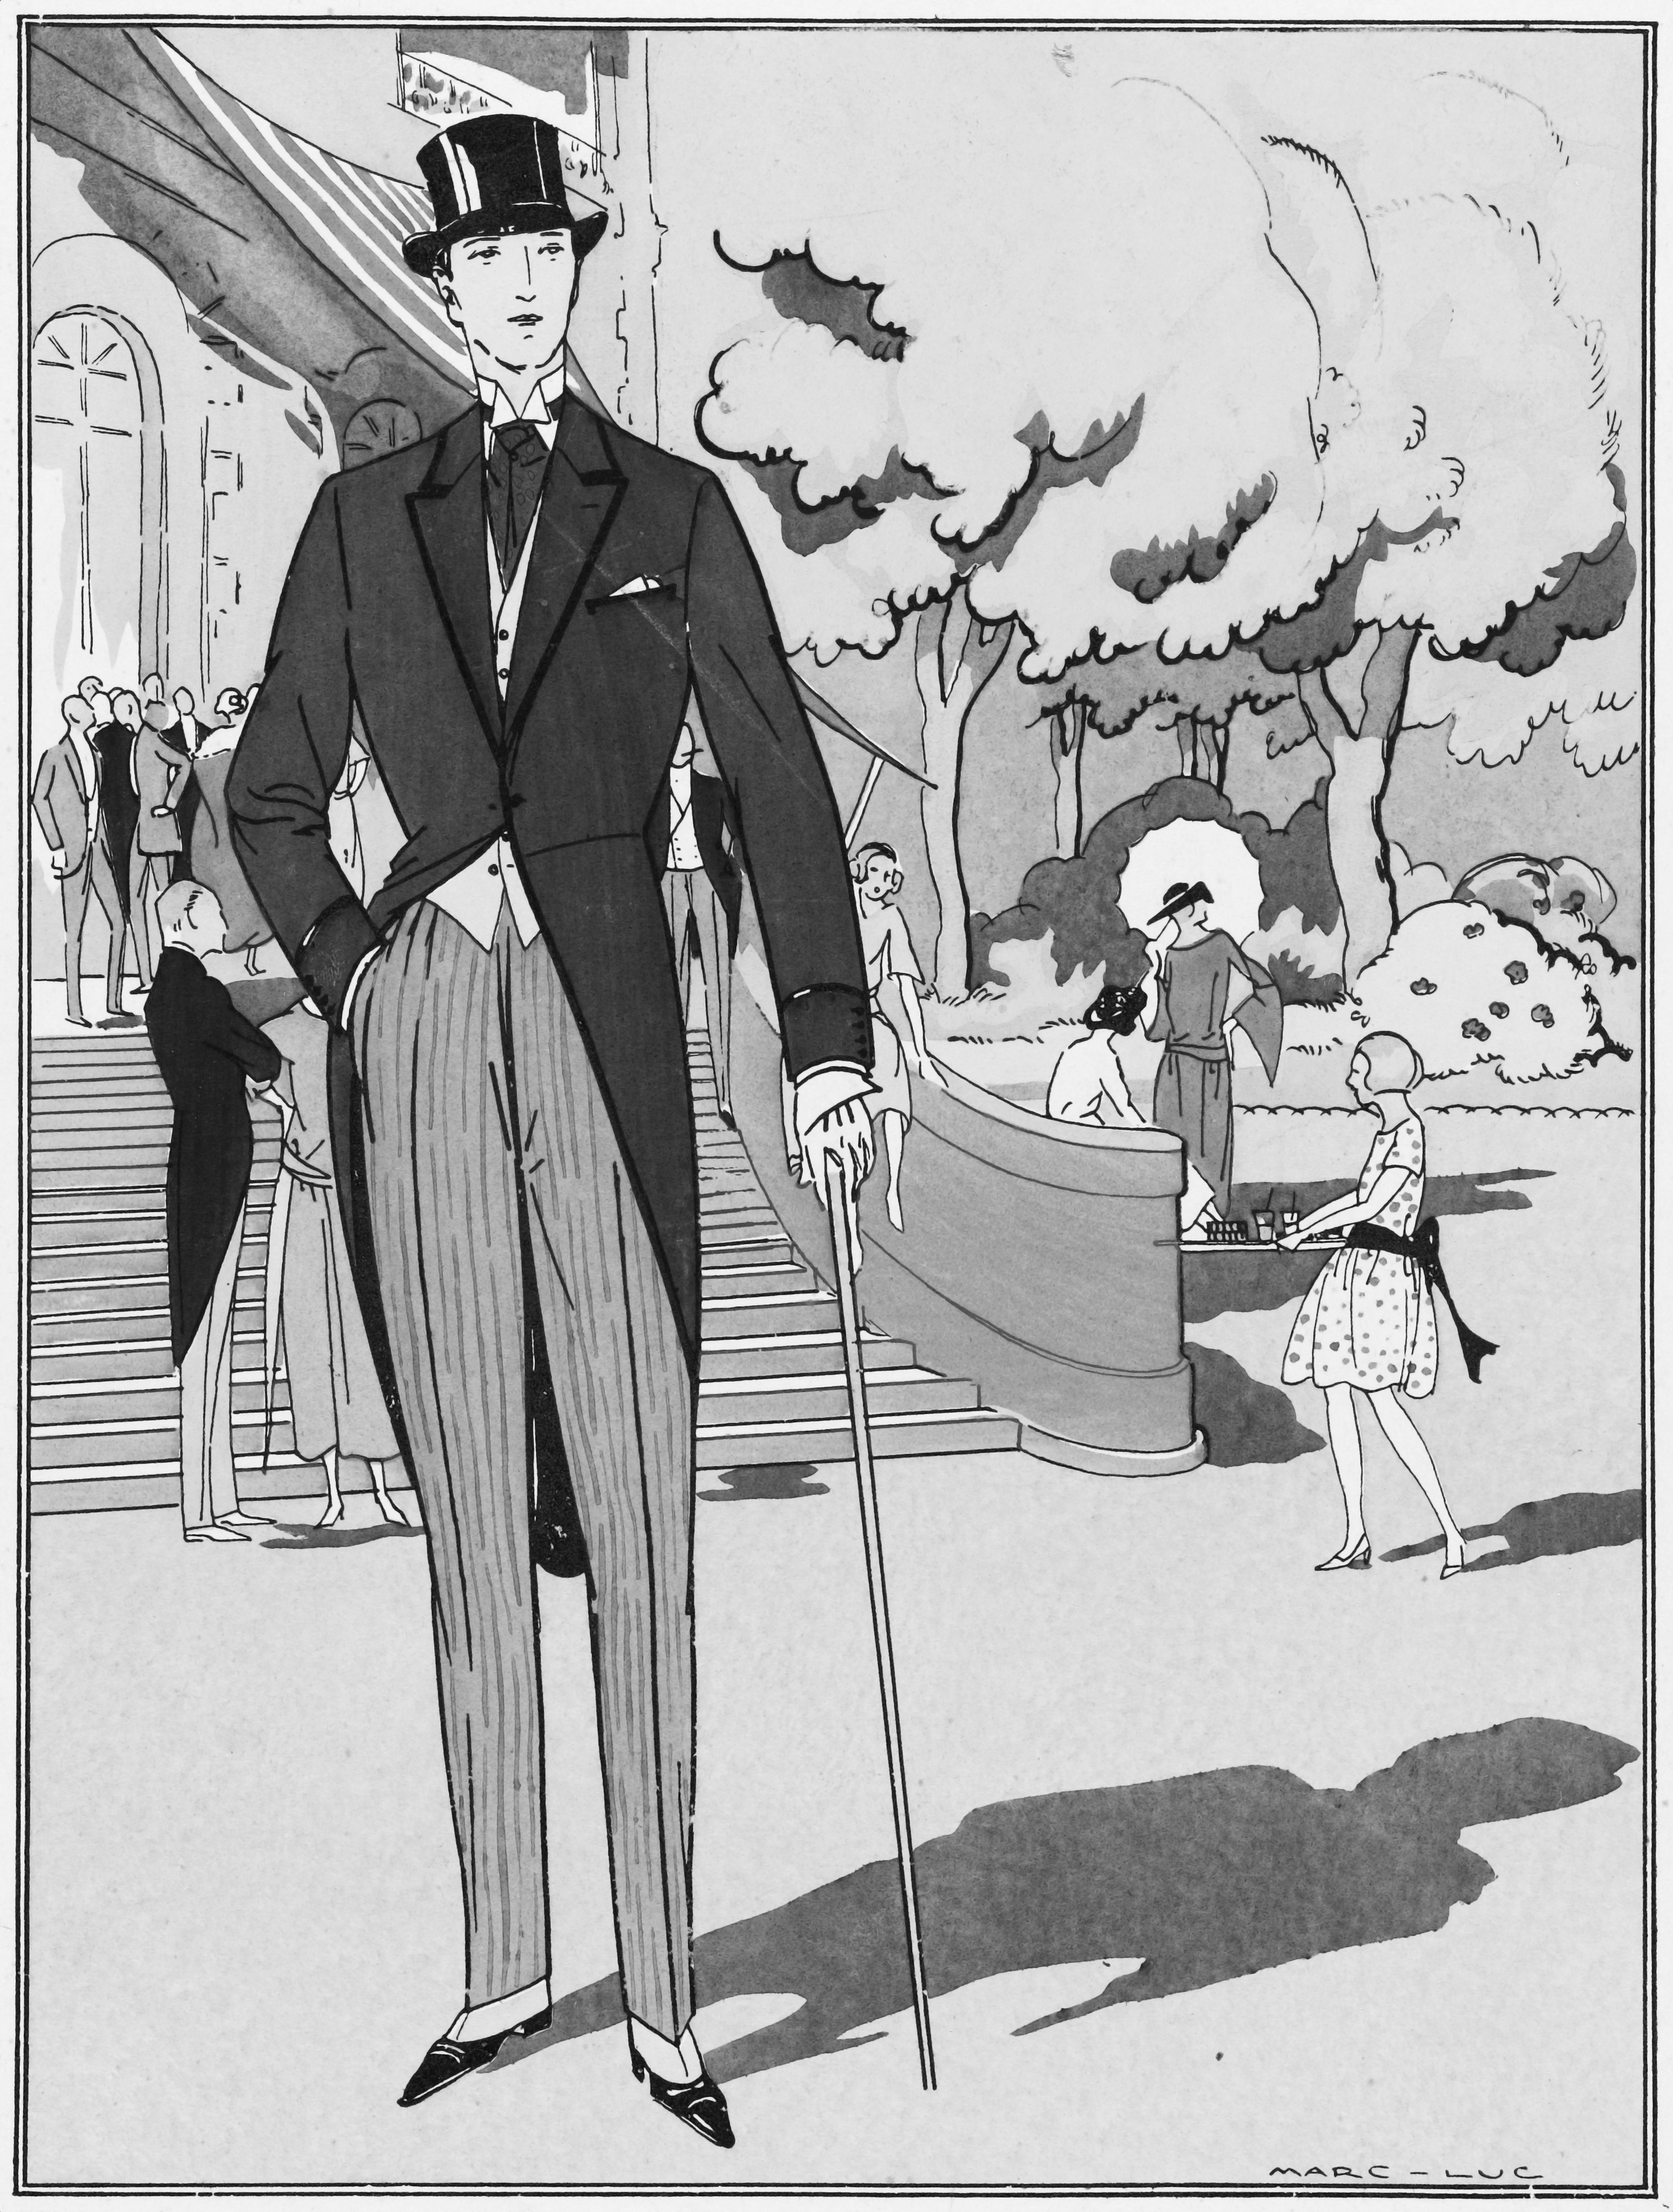
\includegraphics[width=\coverimagesize]{summer1923}\\
 \end{center}
 \vspace*{.1cm}
 \begin{center}\setstretch{1.5}\myauthorfont
{\setstretch{1.5}\reasonablyhuge Dorothy L. Sayers}\\
\end{center}
\end{titlepage}

  \recalctypearea
\restoregeometry



\pagestyle{plain}

\renewcommand*\raggedchapter{\centering}



\KOMAoptions{headings=openleft}


%\vspace*{-2\baselineskip}
\tableofcontents
\clearpage


%\clearpage






\mainmatter
\pagestyle{headings}
\renewcommand*{\chapterpagestyle}{plain}

\KOMAoptions{headings=openright}
%!TeX root=../bodytop.tex
\chapter[Chapter \thechapter]{}
\lettrine[lines=4,ante=‘]{O}{h}, damn!' said Lord~Peter Wimsey at Piccadilly Circus. <Hi, driver!>

\zz
The taxi man, irritated at receiving this appeal while negotiating the intricacies of turning into Lower Regent Street across the route of a 19 'bus, a 38-B and a bicycle, bent an unwilling ear.

<I've left the catalogue behind,> said Lord~Peter deprecatingly. <Uncommonly careless of me. D'you mind puttin' back to where we came from?>

<To the Savile Club, sir?>

<No—110 Piccadilly—just beyond—thank you.>

<Thought you was in a hurry,> said the man, overcome with a sense of injury.

<I'm afraid it's an awkward place to turn in,> said Lord~Peter, answering the thought rather than the words. His long, amiable face looked as if it had generated spontaneously from his top hat, as white maggots breed from Gorgonzola.

The taxi, under the severe eye of a policeman, revolved by slow jerks, with a noise like the grinding of teeth.

The block of new, perfect and expensive flats in which Lord~Peter dwelt upon the second floor, stood directly opposite the Green Park, in a spot for many years occupied by the skeleton of a frustrate commercial enterprise. As Lord~Peter let himself in he heard his man's voice in the library, uplifted in that throttled stridency peculiar to well-trained persons using the telephone.

<I believe that's his lordship just coming in again—if your Grace would kindly hold the line a moment.>

<What is it, Bunter?>

<Her Grace has just called up from Denver, my lord. I was just saying your lordship had gone to the sale when I heard your lordship's latchkey.>

<Thanks,> said Lord~Peter; <and you might find me my catalogue, would you? I think I must have left it in my bedroom, or on the desk.>

He sat down to the telephone with an air of leisurely courtesy, as though it were an acquaintance dropped in for a chat.

<Hullo, Mother—that you?>

<Oh, there you are, dear,> replied the voice of the Dowager Duchess. <I was afraid I'd just missed you.>

<Well, you had, as a matter of fact. I'd just started off to Brocklebury's sale to pick up a book or two, but I had to come back for the catalogue. What's up?>

<Such a quaint thing,> said the Duchess. <I thought I'd tell you. You know little Mr~Thipps?>

<Thipps?> said Lord~Peter. <Thipps? Oh, yes, the little architect man who's doing the church roof. Yes. What about him?>

<Mrs~Throgmorton's just been in, in quite a state of mind.>

<Sorry, Mother, I can't hear. Mrs~Who?>

<Throgmorton—Throgmorton—the vicar's wife.>

<Oh, Throgmorton, yes?>

<Mr~Thipps rang them up this morning. It was his day to come down, you know.>

<Yes?>

<He rang them up to say he couldn't. He was so upset, poor little man. He'd found a dead body in his bath.>

<Sorry, Mother, I can't hear; found what, where?>

<A dead body, dear, in his bath.>

<What?—no, no, we haven't finished. Please don't cut us off. Hullo! Hullo! Is that you, Mother? Hullo!—Mother!—Oh, yes—sorry, the girl was trying to cut us off. What sort of body?>

<A dead man, dear, with nothing on but a pair of pince-nez. Mrs~Throgmorton positively blushed when she was telling me. I'm afraid people do get a little narrow-minded in country vicarages.>

<Well, it sounds a bit unusual. Was it anybody he knew?>

<No, dear, I don't think so, but, of course, he couldn't give her many details. She said he sounded quite distracted. He's such a respectable little man—and having the police in the house and so on, really worried him.>

<Poor little Thipps! Uncommonly awkward for him. Let's see, he lives in Battersea, doesn't he?>

<Yes, dear; 59, Queen Caroline Mansions; opposite the Park. That big block just round the corner from the Hospital. I thought perhaps you'd like to run round and see him and ask if there's anything we can do. I always thought him a nice little man.>

<Oh, quite,> said Lord~Peter, grinning at the telephone. The Duchess was always of the greatest assistance to his hobby of criminal investigation, though she never alluded to it, and maintained a polite fiction of its non-existence.

<What time did it happen, Mother?>

<I think he found it early this morning, but, of course, he didn't think of telling the Throgmortons just at first. She came up to me just before lunch—so tiresome, I had to ask her to stay. Fortunately, I was alone. I don't mind being bored myself, but I hate having my guests bored.>

<Poor old Mother! Well, thanks awfully for tellin' me. I think I'll send Bunter to the sale and toddle round to Battersea now an' try and console the poor little beast. So-long.>

<Good-bye, dear.>

<Bunter!>

<Yes, my lord.>

<Her Grace tells me that a respectable Battersea architect has discovered a dead man in his bath.>

<Indeed, my lord? That's very gratifying.>

<Very, Bunter. Your choice of words is unerring. I wish Eton and Balliol had done as much for me. Have you found the catalogue?>

<Here it is, my lord.>

<Thanks. I am going to Battersea at once. I want you to attend the sale for me. Don't lose time—I don't want to miss the Folio Dante\footnote{This is the first Florence edition, 1481, by Niccolo di Lorenzo. Lord~Peter's collection of printed Dantes is worth inspection. It includes, besides the famous Aldine 8vo. of 1502, the Naples folio of 1477—<edizione rarissima>, according to Colomb. This copy has no history, and Mr~Parker's private belief is that its present owner conveyed it away by stealth from somewhere or other. Lord~Peter's own account is that he <picked it up in a little place in the hills>, when making a walking-tour through Italy.} nor the de Voragine—here you are—see? \textit{Golden Legend}—Wynkyn de Worde, 1493—got that?—and, I say, make a special effort for the Caxton folio of the \textit{Four Sons of Aymon}—it's the 1489 folio and unique. Look! I've marked the lots I want, and put my outside offer against each. Do your best for me. I shall be back to dinner.>

<Very good, my lord.>

<Take my cab and tell him to hurry. He may for you; he doesn't like me very much. Can I\@,> said Lord~Peter, looking at himself in the eighteenth-century mirror over the mantelpiece, <can I have the heart to fluster the flustered Thipps further—that's very difficult to say quickly—by appearing in a top-hat and frock-coat? I think not. Ten to one he will overlook my trousers and mistake me for the undertaker. A grey suit, I fancy, neat but not gaudy, with a hat to tone, suits my other self better. Exit the amateur of first editions; new motive introduced by solo bassoon; enter Sherlock Holmes, disguised as a walking gentleman. There goes Bunter. Invaluable fellow—never offers to do his job when you've told him to do somethin' else. Hope he doesn't miss the \textit{Four Sons of Aymon}. Still, there \textit{is} another copy of that—in the Vatican.\footnote{Lord~Peter's wits were wool-gathering. The book is in the possession of Earl Spencer. The Brocklebury copy is incomplete, the last five signatures being altogether missing, but is unique in possessing the colophon.} It might become available, you never know—if the Church of Rome went to pot or Switzerland invaded Italy—whereas a strange corpse doesn't turn up in a suburban bathroom more than once in a lifetime—at least, I should think not—at any rate, the number of times it's happened, \textit{with} a pince-nez, might be counted on the fingers of one hand, I imagine. Dear me! it's a dreadful mistake to ride two hobbies at once.>

He had drifted across the passage into his bedroom, and was changing with a rapidity one might not have expected from a man of his mannerisms. He selected a dark-green tie to match his socks and tied it accurately without hesitation or the slightest compression of his lips; substituted a pair of brown shoes for his black ones, slipped a monocle into a breast pocket, and took up a beautiful Malacca walking-stick with a heavy silver knob.

<That's all, I think,> he murmured to himself. <Stay—I may as well have you—you may come in useful—one never knows.> He added a flat silver matchbox to his equipment, glanced at his watch, and seeing that it was already a quarter to three, ran briskly downstairs, and, hailing a taxi, was carried to Battersea Park.

Mr~Alfred Thipps was a small, nervous man, whose flaxen hair was beginning to abandon the unequal struggle with destiny. One might say that his only really marked feature was a large bruise over the left eyebrow, which gave him a faintly dissipated air incongruous with the rest of his appearance. Almost in the same breath with his first greeting, he made a self-conscious apology for it, murmuring something about having run against the dining-room door in the dark. He was touched almost to tears by Lord~Peter's thoughtfulness and condescension in calling.

<I'm sure it's most kind of your lordship,> he repeated for the dozenth time, rapidly blinking his weak little eyelids. <I appreciate it very deeply, very deeply, indeed, and so would Mother, only she's so deaf, I don't like to trouble you with making her understand. It's been very hard all day,> he added, <with the policemen in the house and all this commotion. It's what Mother and me have never been used to, always living very retired, and it's most distressing to a man of regular habits, my lord, and reely, I'm almost thankful Mother doesn't understand, for I'm sure it would worry her terribly if she was to know about it. She was upset at first, but she's made up some idea of her own about it now, and I'm sure it's all for the best.>

The old lady who sat knitting by the fire nodded grimly in response to a look from her son.

<I always said as you ought to complain about that bath, Alfred,> she said suddenly, in the high, piping voice peculiar to the deaf, <and it's to be 'oped the landlord'll see about it now; not but what I think you might have managed without having the police in, but there! you always were one to make a fuss about a little thing, from chicken-pox up.>

<There now,> said Mr~Thipps apologetically, <you see how it is. Not but what it's just as well she's settled on that, because she understands we've locked up the bathroom and don't try to go in there. But it's been a terrible shock to me, sir—my lord, I should say, but there! my nerves are all to pieces. Such a thing has never 'appened—happened to me in all my born days. Such a state I was in this morning—I didn't know if I was on my head or my heels—I reely didn't, and my heart not being too strong, I hardly knew how to get out of that horrid room and telephone for the police. It's affected me, sir, it's affected me, it reely has—I couldn't touch a bit of breakfast, nor lunch neither, and what with telephoning and putting off clients and interviewing people all morning, I've hardly known what to do with myself.>

<I'm sure it must have been uncommonly distressin',> said Lord~Peter, sympathetically, <especially comin' like that before breakfast. Hate anything tiresome happenin' before breakfast. Takes a man at such a confounded disadvantage, what?>

<That's just it, that's just it,> said Mr~Thipps, eagerly. <When I saw that dreadful thing lying there in my bath, mother-naked, too, except for a pair of eyeglasses, I assure you, my lord, it regularly turned my stomach, if you'll excuse the expression. I'm not very strong, sir, and I get that sinking feeling sometimes in the morning, and what with one thing and another I 'ad—had to send the girl for a stiff brandy, or I don't know \textit{what} mightn't have happened. I felt so queer, though I'm anything but partial to spirits as a rule. Still, I make it a rule never to be without brandy in the house, in case of emergency, you know?>

<Very wise of you,> said Lord~Peter, cheerfully. <You're a very far-seein' man, Mr~Thipps. Wonderful what a little nip'll do in case of need, and the less you're used to it the more good it does you. Hope your girl is a sensible young woman, what? Nuisance to have women faintin' and shriekin' all over the place.>

<Oh, Gladys is a good girl,> said Mr~Thipps, <very reasonable indeed. She was shocked, of course; that's very understandable. I was shocked myself, and it wouldn't be proper in a young woman not to be shocked under the circumstances, but she is reely a helpful, energetic girl in a crisis, if you understand me. I consider myself very fortunate these days to have got a good, decent girl to do for me and Mother, even though she is a bit careless and forgetful about little things, but that's only natural. She was very sorry indeed about having left the bathroom window open, she reely was, and though I was angry at first, seeing what's come of it, it wasn't anything to speak of, not in the ordinary way, as you might say. Girls will forget things, you know, my lord, and reely she was so distressed I didn't like to say too much to her. All I said was: <It might have been burglars,> I said, <remember that, next time you leave a window open all night; this time it was a dead man,> I said, <and that's unpleasant enough, but next time it might be burglars,> I said, <and all of us murdered in our beds.> But the police-inspector—Inspector~Sugg, they called him, from the Yard—he was very sharp with her, poor girl. Quite frightened her, and made her think he suspected her of something, though what good a body could be to her, poor girl, I can't imagine, and so I told the Inspector. He was quite rude to me, my lord—I may say I didn't like his manner at all. <If you've got anything definite to accuse Gladys or me of, Inspector,> I said to him, <bring it forward, that's what you have to do,> I said, <but I've yet to learn that you're paid to be rude to a gentleman in his own 'ouse—house.> Reely,> said Mr~Thipps, growing quite pink on the top of his head, <he regularly roused me, regularly roused me, my lord, and I'm a mild man as a rule.>

<Sugg all over,> said Lord~Peter. <I know him. When he don't know what else to say, he's rude. Stands to reason you and the girl wouldn't go collectin' bodies. Who'd want to saddle himself with a body? Difficulty's usually to get rid of 'em. Have you got rid of this one yet, by the way?>

<It's still in the bathroom,> said Mr~Thipps. <Inspector~Sugg said nothing was to be touched till his men came in to move it. I'm expecting them at any time. If it would interest your lordship to have a look at it\longdash>

<Thanks awfully,> said Lord~Peter. <I'd like to very much, if I'm not puttin' you out.>

<Not at all,> said Mr~Thipps. His manner as he led the way along the passage convinced Lord~Peter of two things—first, that, gruesome as his exhibit was, he rejoiced in the importance it reflected upon himself and his flat, and secondly, that Inspector~Sugg had forbidden him to exhibit it to anyone. The latter supposition was confirmed by the action of Mr~Thipps, who stopped to fetch the door-key from his bedroom, saying that the police had the other, but that he made it a rule to have two keys to every door, in case of accident.

The bathroom was in no way remarkable. It was long and narrow, the window being exactly over the head of the bath. The panes were of frosted glass; the frame wide enough to admit a man's body. Lord~Peter stepped rapidly across to it, opened it and looked out.

The flat was the top one of the building and situated about the middle of the block. The bathroom window looked out upon the back-yards of the flats, which were occupied by various small outbuildings, coal-holes, garages, and the like. Beyond these were the back gardens of a parallel line of houses. On the right rose the extensive edifice of St~Luke's Hospital, Battersea, with its grounds, and, connected with it by a covered way, the residence of the famous surgeon, Sir Julian Freke, who directed the surgical side of the great new hospital, and was, in addition, known in Harley Street as a distinguished neurologist with a highly individual point of view.

This information was poured into Lord~Peter's ear at considerable length by Mr~Thipps, who seemed to feel that the neighbourhood of anybody so distinguished shed a kind of halo of glory over Queen Caroline Mansions.

<We had him round here himself this morning,> he said, <about this horrid business. Inspector~Sugg thought one of the young medical gentlemen at the hospital might have brought the corpse round for a joke, as you might say, they always having bodies in the dissecting-room. So Inspector~Sugg went round to see Sir Julian this morning to ask if there was a body missing. He was very kind, was Sir Julian, very kind indeed, though he was at work when they got there, in the dissecting-room. He looked up the books to see that all the bodies were accounted for, and then very obligingly came round here to look at this>—he indicated the bath—<and said he was afraid he couldn't help us—there was no corpse missing from the hospital, and this one didn't answer to the description of any they'd had.>

<Nor to the description of any of the patients, I hope,> suggested Lord~Peter casually.

At this grisly hint Mr~Thipps turned pale.

<I didn't hear Inspector~Sugg inquire,> he said, with some agitation. <What a very horrid thing that would be—God bless my soul, my lord, I never thought of it.>

<Well, if they had missed a patient they'd probably have discovered it by now,> said Lord~Peter. <Let's have a look at this one.>

He screwed his monocle into his eye, adding: <I see you're troubled here with the soot blowing in. Beastly nuisance, ain't it? I get it, too—spoils all my books, you know. Here, don't you trouble, if you don't care about lookin' at it.>

He took from Mr~Thipps's hesitating hand the sheet which had been flung over the bath, and turned it back.

The body which lay in the bath was that of a tall, stout man of about fifty. The hair, which was thick and black and naturally curly, had been cut and parted by a master hand, and exuded a faint violet perfume, perfectly recognisable in the close air of the bathroom. The features were thick, fleshy and strongly marked, with prominent dark eyes, and a long nose curving down to a heavy chin. The clean-shaven lips were full and sensual, and the dropped jaw showed teeth stained with tobacco. On the dead face the handsome pair of gold pince-nez mocked death with grotesque elegance; the fine gold chain curved over the naked breast. The legs lay stiffly stretched out side by side; the arms reposed close to the body; the fingers were flexed naturally. Lord~Peter lifted one arm, and looked at the hand with a little frown.

<Bit of a dandy, your visitor, what?> he murmured. <Parma violet and manicure.> He bent again, slipping his hand beneath the head. The absurd eyeglasses slipped off, clattering into the bath, and the noise put the last touch to Mr~Thipps's growing nervousness.

<If you'll excuse me,> he murmured, <it makes me feel quite faint, it reely does.>

He slipped outside, and he had no sooner done so than Lord~Peter, lifting the body quickly and cautiously, turned it over and inspected it with his head on one side, bringing his monocle into play with the air of the late Joseph Chamberlain approving a rare orchid. He then laid the head over his arm, and bringing out the silver matchbox from his pocket, slipped it into the open mouth. Then making the noise usually written <Tut-tut,> he laid the body down, picked up the mysterious pince-nez, looked at it, put it on his nose and looked through it, made the same noise again, readjusted the pince-nez upon the nose of the corpse, so as to leave no traces of interference for the irritation of Inspector~Sugg; rearranged the body; returned to the window and, leaning out, reached upwards and sideways with his walking-stick, which he had somewhat incongruously brought along with him. Nothing appearing to come of these investigations, he withdrew his head, closed the window, and rejoined Mr~Thipps in the passage.

Mr~Thipps, touched by this sympathetic interest in the younger son of a duke, took the liberty, on their return to the sitting-room, of offering him a cup of tea. Lord~Peter, who had strolled over to the window and was admiring the outlook on Battersea Park, was about to accept, when an ambulance came into view at the end of Prince of Wales Road. Its appearance reminded Lord~Peter of an important engagement, and with a hurried <By Jove!> he took his leave of Mr~Thipps.

<My mother sent kind regards and all that,> he said, shaking hands fervently; <hopes you'll soon be down at Denver again. Good-bye, Mrs~Thipps,> he bawled kindly into the ear of the old lady. <Oh, no, my dear sir, please don't trouble to come down.>

He was none too soon. As he stepped out of the door and turned towards the station, the ambulance drew up from the other direction, and Inspector~Sugg emerged from it with two constables. The Inspector~spoke to the officer on duty at the Mansions, and turned a suspicious gaze on Lord~Peter's retreating back.

<Dear old Sugg,> said that nobleman, fondly, <dear, dear old bird! How he does hate me, to be sure.>
%!TeX root=../bellonatop.tex
\chapter{The Queen is Out}
\lettrine[lines=4]{I}{t} is doubtful which occurrence was more disagreeable to the senior members of the Bellona Club—the grotesque death of General Fentiman in their midst or the indecent neurasthenia of his grandson. Only the younger men felt no sense of outrage; they knew too much. Dick Challoner—known to his intimates as Tin-Tummy Challoner, owing to the fact that he had been fitted with a spare part after the second battle of the Somme—took the gasping Fentiman away into the deserted library for a stiffener. The Club Secretary hurried in, in his dress-shirt and trousers, the half-dried lather still clinging to his jaws. After one glance he sent an agitated waiter to see if Dr~Penberthy was still in the Club. Colonel Marchbanks laid a large silk handkerchief reverently over the rigid face in the arm-chair and remained quietly standing. A little circle formed about the edge of the hearthrug, not quite certain what to do. From time to time it was swelled by fresh arrivals, whom the news had greeted in the hall as they wandered in. A little group appeared from the bar. »What? old Fentiman?« they said. »Good God, you don't say so. Poor old blighter. Heart gone at last, I suppose«; and they extinguished cigars and cigarettes, and stood by, not liking to go away again.

Dr~Penberthy was just changing for dinner. He came down hurriedly, caught just as he was going out to an Armistice dinner, his silk hat tilted to the back of his head, his coat and muffler pushed loosely open. He was a thin, dark man with the abrupt manner which distinguishes the Army Surgeon from the West-end practitioner. The group by the fire made way for him, except Wimsey, who hung rather foolishly upon the big elbow-chair, gazing in a helpless way at the body.

Penberthy ran practised hands quickly over neck, wrists and knee-joints.

»Dead several hours,« he pronounced, sharply. »Rigour well-established—beginning to pass off.« He moved the dead man's left leg in illustration; it swung loose at the knee. »I've been expecting this. Heart very weak. Might happen any moment. Any one spoken to him to-day?«

He glanced around interrogatively.

»I saw him here after lunch,« volunteered somebody. »I didn't speak.«

»I thought he was asleep,« said another.

Nobody remembered speaking to him. They were so used to old General Fentiman, slumbering by the fire.

»Ah, well,« said the doctor. »What's the time? Seven?« He seemed to make a rapid calculation. »Say five hours for rigour to set in—must have taken place very rapidly—he probably came in at his usual time, sat down and died straight away.«

»He always walked from Dover Street,« put in an elderly man, »I told him it was too great an exertion at his age. You've heard me say so, Ormsby.«

»Yes, yes, quite,« said the purple-faced Ormsby. »Dear me, just so.«

»Well, there's nothing to be done,« said the doctor. »Died in his sleep. Is there an empty bedroom we can take him to, Culyer?«

»Yes, certainly,« said the Secretary. »James, fetch the key of number sixteen from my office and tell them to put the bed in order. I suppose, eh, doctor?—when the rigour passes off we shall be able to—eh?«

»Oh, yes, you'll be able to do everything that's required. I'll send the proper people in to lay him out for you. Somebody had better let his people know—only they'd better not show up till we can get him more presentable.«

»Captain Fentiman knows already,« said Colonel Marchbanks. »And Major Fentiman is staying in the Club—he'll probably be in before long. Then there's a sister, I think.«

»Yes, old Lady Dormer,« said Penberthy, »she lives round in Portman Square. They haven't been on speaking terms for years. Still, she'll have to know.«

»I'll ring them up,« said the Colonel. »We can't leave it to Captain Fentiman, he's in no fit state to be worried, poor fellow. You'll have to have a look at him, doctor, when you've finished here. An attack of the old trouble—nerves, you know.«

»All right. Ah! is the room ready, Culyer? Then we'll move him. Will somebody take his shoulders—no, not you, Culyer« (for the Secretary had only one sound arm), »Lord~Peter, yes, thank you—lift carefully.«

Wimsey put his long, strong hands under the stiff arms; the doctor gathered up the legs; they moved away. They looked like a dreadful little Guy Fawkes procession, with that humped and unreverend mannikin bobbing and swaying between them.

The door closed after them, and a tension seemed removed. The circle broke up into groups. Somebody lit a cigarette. The planet's tyrant, dotard Death, had held his gray mirror before them for a moment and shown them the image of things to come. But now it was taken away again. The unpleasantness had passed. Fortunate, indeed, that Penberthy was the old man's own doctor. He knew all about it. He could give a certificate. No inquest. Nothing undesirable. The members of the Bellona Club could go to dinner.

Colonel Marchbanks turned to go through the far door towards the library. In a narrow ante-room between the two rooms there was a convenient telephone cabinet for the use of those members who did not wish to emerge into the semi-publicity of the entrance-hall.

»Hi, colonel! not that one. That instrument's out of order,« said a man called Wetheridge, who saw him go. »Disgraceful, I call it. I wanted to use the 'phone this morning, and—oh! hullo! the notice has gone. I suppose it's all right again. They ought to let one know.«

Colonel Marchbanks paid little attention to Wetheridge. He was the club grumbler, distinguished even in that fellowship of the dyspeptic and peremptory—always threatening to complain to the Committee, harassing the Secretary and constituting a perennial thorn in the sides of his fellow-members. He retired, murmuring, to his chair and the evening paper, and the Colonel stepped into the telephone cabinet to call up Lady Dormer's house in Portman Square.

Presently he came out through the library into the entrance-hall, and met Penberthy and Wimsey just descending the staircase.

»Have you broken the news to Lady Dormer?« asked Wimsey.

»Lady Dormer is dead,« said the Colonel. »Her maid tells me she passed quietly away at half-past ten this morning.«
%!TeX root=../bellonatop.tex
\chapter{Hearts Count More Than Diamonds}
\lettrine[lines=4]{A}{bout} ten days after that notable Armistice Day, Lord Peter Wimsey was sitting in his library, reading a rare fourteenth century manuscript of Justinian. It gave him particular pleasure, being embellished with a large number of drawings in sepia, extremely delicate in workmanship, and not always equally so in subject. Beside him on a convenient table stood a long-necked decanter of priceless old port. From time to time he stimulated his interest with a few sips, pursing his lips thoughtfully, and slowly savoring the balmy after-taste.

A ring at the front door of the flat caused him to exclaim \enquote{Oh, hell!} and cock an attentive ear for the intruder's voice. Apparently the result was satisfactory, for he closed the Justinian and had assumed a welcoming smile when the door opened.

\enquote{Mr Murbles, my lord.}

The little elderly gentleman who entered was so perfectly the family solicitor as really to have no distinguishing personality at all, beyond a great kindliness of heart and a weakness for soda-mint lozenges.

\enquote{I am not disturbing you, I trust, Lord Peter.}

\enquote{Good lord, no, sir. Always delighted to see you. Bunter, a glass for Mr Murbles. Very glad you've turned up, sir. The Cockburn '80 always tastes a lot better in company\allowbreak---\allowbreak discernin' company, that is. Once knew a fellow who polluted it with a Trichinopoly. He was not asked again. Eight months later, he committed suicide. I don't say it was on that account. But he was earmarked for a bad end, what?}

\enquote{You horrify me,} said Mr Murbles, gravely. \enquote{I have seen many men sent to the gallows for crimes with which I could feel much more sympathy. Thank you, Bunter, thank you. You are quite well, I trust?}

\enquote{I am in excellent health, I am obliged to you, sir.}

\enquote{That's good. Been doing any photography lately?}

\enquote{A certain amount, sir. But merely of a pictorial description, if I may venture to call it so. Criminological material, sir, has been distressingly deficient of late.}

\enquote{Perhaps Mr Murbles has brought us something,} suggested Wimsey.

\enquote{No,} said Mr Murbles, holding the Cockburn '80 beneath his nostrils and gently agitating the glass to release the ethers, \enquote{no, I can't say I have, precisely. I will not disguise that I have come in the hope of deriving benefit from your trained habits of observation and deduction, but I fear\allowbreak---\allowbreak that is, I trust\allowbreak---\allowbreak in fact, I am confident\allowbreak---\allowbreak that nothing of an undesirable nature is involved. The fact is,} he went on, as the door closed upon the retreating Bunter, \enquote{a curious question has arisen with regard to the sad death of General Fentiman at the Bellona Club, to which, I understand, you were a witness.}

\enquote{If you understand that, Murbles,} said his lordship, cryptically, \enquote{you understand a damn sight more than I do. I did not witness the death\allowbreak---\allowbreak I witnessed the discovery of the death\allowbreak---\allowbreak which is a very different thing, by a long chalk.}

\enquote{By how long a chalk?} asked Mr Murbles, eagerly. \enquote{That is just what I am trying to find out.}

\enquote{That's very inquisitive of you,} said Wimsey. \enquote{I think perhaps it would be better ...} he lifted his glass and tilted it thoughtfully, watching the wine coil down in thin flower-petallings from rim to stem ... \enquote{if you were to tell me exactly what you want to know ... and why. After all ... I'm a member of the Club ... family associations chiefly, I suppose ... but there it is.}

Mr Murbles looked up sharply, but Wimsey's attention seemed focussed upon the port.

\enquote{Quite so,} said the solicitor. \enquote{Very well. The facts of the matter are these. General Fentiman had, as you know, a sister Felicity, twelve years younger than himself. She was very beautiful and very willful as a girl, and ought to have made a very fine match, but for the fact that the Fentimans, though extremely well-descended, were anything but well-off. As usual at that period, all the money there was went to educating the boy, buying him a commission in a crack regiment and supporting him there in the style which was considered indispensable for a Fentiman. Consequently there was nothing left to furnish a marriage-portion for Felicity, and that was rather disastrous for a young woman sixty years ago.

Well, Felicity got tired of being dragged through the social round in her darned muslins and gloves that had been to the cleaners\allowbreak---\allowbreak and she had the spirit to resent her mother's perpetual strategies in the match-making line. There was a dreadful, decrepit old viscount, eaten up with diseases and dissipations, who would have been delighted to totter to the altar with a handsome young creature of eighteen, and I am sorry to say that the girl's father and mother did everything they could to force her into accepting this disgraceful proposal. In fact, the engagement was announced and the wedding-day fixed, when, to the extreme horror of her family, Felicity calmly informed them one morning that she had gone out before breakfast and actually got married, in the most indecent secrecy and haste, to a middle-aged man called Dormer, very honest and abundantly wealthy, and\allowbreak---\allowbreak horrid to relate\allowbreak---\allowbreak a prosperous manufacturer. Buttons, in fact\allowbreak---\allowbreak made of papier mâché or something, with a patent indestructible shank\allowbreak---\allowbreak were the revolting antecedents to which this head-strong young Victorian had allied herself.

Naturally there was a terrible scandal, and the parents did their best\allowbreak---\allowbreak seeing that Felicity was a minor\allowbreak---\allowbreak to get the marriage annulled. However, Felicity checkmated their plans pretty effectually by escaping from her bedroom\allowbreak---\allowbreak I fear, indeed, that she actually climbed down a tree in the back-garden, crinoline and all\allowbreak---\allowbreak and running away with her husband. After which, seeing that the worst had happened\allowbreak---\allowbreak indeed, Dormer, a man of prompt action, lost no time in putting his bride in the family way\allowbreak---\allowbreak the old people put the best face they could on it in the grand Victorian manner. That is, they gave their consent to the marriage, forwarded their daughter's belongings to her new home in Manchester, and forbade her to darken their doors again.}

\enquote{Highly proper,} murmured Wimsey. \enquote{I'm determined never to be a parent. Modern manners and the break-up of the fine old traditions have simply ruined the business. I shall devote my life and fortune to the endowment of research on the best method of producin' human beings decorously and unobtrusively from eggs. All parental responsibility to devolve upon the incubator.}

\enquote{I hope not,} said Mr Murbles. \enquote{My own profession is largely supported by domestic entanglements. To proceed. Young Arthur Fentiman seems to have shared the family views. He was disgusted at having a brother-in-law in buttons, and the jests of his mess-mates did nothing to sweeten his feelings toward his sister. He became impenetrably military and professional, crusted over before his time, and refused to aknowledge the existence of anybody called Dormer. Mind you, the old boy was a fine soldier, and absolutely wrapped up in his Army associations. In due course he married\allowbreak---\allowbreak not well, for he had not the means to entitle himself to a noble wife, and he would not demean himself by marrying money, like the unspeakable Felicity. He married a suitable gentlewoman with a few thousand pounds. She died (largely, I believe, owing to the military regularity with which her husband ordained that she should perform her maternal functions), leaving a numerous but feeble family of children. Of these, the only one to attain maturity was the father of the two Fentimans you know\allowbreak---\allowbreak Major Robert and Captain George Fentiman.}

\enquote{I don't know Robert very well,} interjected Wimsey. \enquote{I've met him. Frightfully hearty and all that\allowbreak---\allowbreak regular army type.}

\enquote{Yes, he's of the old Fentiman stock. Poor George inherited a weakly strain from his grandmother, I'm afraid.}

\enquote{Well, nervous, anyhow,} said Wimsey, who knew better than the old solicitor the kind of mental and physical strain George Fentiman had undergone. The War pressed hardly upon imaginative men in responsible positions. \enquote{And then he was gassed and all that, you know,} he added, apologetically.

\enquote{Just so,} said Mr Murbles. \enquote{Robert, you know, is unmarried and still in the Army. He's not particularly well-off, naturally, for none of the Fentimans ever had a bean, as I believe one says nowadays; but he does very well. George\longdash}

\enquote{Poor old George! All right, sir, you needn't tell me about him. Usual story. Decentish job\allowbreak---\allowbreak imprudent marriage\allowbreak---\allowbreak chucks everything to join up in 1914\allowbreak---\allowbreak invalided out\allowbreak---\allowbreak job gone\allowbreak---\allowbreak health gone\allowbreak---\allowbreak no money\allowbreak---\allowbreak heroic wife keeping the home-fires burning\allowbreak---\allowbreak general fed-upness. Don't let's harrow our feelings. Take it as read.}

\enquote{Yes, I needn't go into that. Their father is dead, of course, and up till ten days ago there were just two surviving Fentimans of the earlier generation. The old General lived on the small fixed income which came to him through his wife and his retired pension. He had a solitary little flat in Dover Street and an elderly man-servant, and he practically lived at the Bellona Club. And there was his sister, Felicity.}

\enquote{How did she come to be Lady Dormer?}

\enquote{Why, that's where we come to the interesting part of the story. Henry Dormer\longdash}

\enquote{The button-maker?}

\enquote{The button-maker. He became an exceedingly rich man indeed\allowbreak---\allowbreak so rich, in fact, that he was able to offer financial assistance to certain exalted persons who need not be mentioned and so, in time, and in consideration of valuable services to the nation not very clearly specified in the Honors List, he became Sir Henry Dormer, Bart. His only child\allowbreak---\allowbreak a girl\allowbreak---\allowbreak had died, and there was no prospect of any further family, so there was, of course, no reason why he should not be made a baronet for his trouble.}

\enquote{Acid man you are,} said Wimsey. \enquote{No reverence, no simple faith or anything of that kind. Do lawyers ever go to heaven?}

\enquote{I have no information on that point,} said Mr Murbles, dryly. \enquote{Lady Dormer\longdash}

\enquote{Did the marriage turn out well otherwise?} inquired Wimsey.

\enquote{I believe it was perfectly happy,} replied the lawyer, \enquote{an unfortunate circumstance in one way, since it entirely precluded the possibility of any reconciliation with her relatives. Lady Dormer, who was a fine, generous-hearted woman, frequently made overtures of peace, but the General held sternly aloof. So did his son\allowbreak---\allowbreak partly out of respect for the old boy's wishes, but chiefly, I fancy, because he belonged to an Indian regiment and spent most of his time abroad. Robert Fentiman, however, showed the old lady a certain amount of attention, paying occasional visits and so forth, and so did George at one time. Of course they never let the General know a word about it, or he would have had a fit. After the War, George rather dropped his great-aunt\allowbreak---\allowbreak I don't know why.}

\enquote{I can guess,} said Wimsey. \enquote{No job\allowbreak---\allowbreak no money, y' know. Didn't want to look pointed. That sort of thing, what?}

\enquote{Possibly. Or there may have been some kind of quarrel. I don't know. Anyway, those are the facts. I hope I am not boring you, by the way?}

\enquote{I am bearing up,} said Wimsey, \enquote{waiting for the point where the Money comes in. There's a steely legal glitter in your eye, sir, which suggests that the thrill is not far off.}

\enquote{Quite correct,} said Mr Murbles. \enquote{I now come\allowbreak---\allowbreak thank you, well, yes\allowbreak---\allowbreak I will take just one more glass. I thank Providence I am not of a gouty constitution. Yes. Ah!---We now come to the melancholy event of November  11\textsuperscript{th} last, and I must ask you to follow me with the closest attention.}

\enquote{By all means,} said Wimsey, politely.

\enquote{Lady Dormer,} pursued Mr Murbles, leaning earnestly forward, and punctuating every sentence with sharp little jabs of his gold-mounted eye-glasses, held in his right finger and thumb, \enquote{was an old woman, and had been ailing for a very long time. However, she was still the same head-strong and vivacious personality that she had been as a girl, and on the fifth of November she was suddenly seized with a fancy to go out at night and see a display of fireworks at the Crystal Palace or some such place\allowbreak---\allowbreak it may have been Hampstead Heath or the White City\allowbreak---\allowbreak I forget, and it is of no consequence. The important thing is, that it was a raw, cold evening. She insisted on undertaking her little expedition nevertheless, enjoyed the entertainment as heartily as the youngest child, imprudently exposed herself to the night air and caught a severe cold which, in two days' time, turned to pneumonia. On November  10\textsuperscript{th} she was sinking fast, and scarcely expected to live out the night. Accordingly, the young lady who lived with her as her ward\allowbreak---\allowbreak a distant relative, Miss Ann Dorland\allowbreak---\allowbreak sent a message to General Fentiman that if he wished to see his sister alive, he should come immediately. For the sake of our common human nature, I am happy to say that this news broke down the barrier of pride and obstinacy that had kept the old gentleman away so long. He came, found Lady Dormer just conscious, though very feeble, stayed with her about half an hour and departed, still stiff as a ramrod, but visibly softened. This was about four o'clock in the afternoon. Shortly afterwards, Lady Dormer became unconscious, and, indeed, never moved or spoke again, passing peacefully away in her sleep at half-past ten the following morning.

Presumably the shock and nervous strain of the interview with his long-estranged sister had been too much for the old General's feeble system, for, as you know, he died at the Bellona Club at some time\allowbreak---\allowbreak not yet clearly ascertained\allowbreak---\allowbreak on the same day, the eleventh of November.

Now then, at last\allowbreak---\allowbreak and you have been very patient with my tedious way of explaining all this\allowbreak---\allowbreak we come to the point at which we want your help.}

Mr Murbles refreshed himself with a sip of port, and, looking a little anxiously at Wimsey, who had closed his eyes and appeared to be nearly asleep, he resumed.

\enquote{I have not mentioned, I think, how I come to be involved in this matter myself. My father was the Fentimans' family solicitor, a position to which I naturally succeeded when I took over the business at his death. General Fentiman, though he had little enough to leave, was not the sort of disorderly person who dies without making a proper testamentary disposition. His retired pension, of course, died with him, but his small private estate was properly disposed by will. There was a small legacy\allowbreak---\allowbreak fifty pounds\allowbreak---\allowbreak to his man-servant (a very attached and superior fellow); then one or two trifling bequests to old military friends and the servants at the Bellona Club (rings, medals, weapons and small sums of a few pounds each). Then came the bulk of his estate, about \textsterling 2,000, invested in sound securities, and bringing in an income of slightly over \textsterling 100 per annum. These securities, specifically named and enumerated, were left to Captain George Fentiman, the younger grandson, in a very proper clause, which stated that the testator intended no slight in thus passing over the elder one, Major Robert, but that, as George stood in the greater need of monetary help, being disabled, married, and so forth, whereas his brother had his profession and was without ties, George's greater necessity gave him the better claim to such money as there was. Robert was finally named as executor and residuary legatee, thus succeeding to all such personal effects and monies as were not specifically devised elsewhere. Is that clear?}

\enquote{Clear as a bell. Was Robert satisfied with that arrangement?}

\enquote{Oh dear, yes; perfectly. He knew all about the will beforehand and had agreed that it was quite fair and right.}

\enquote{Nevertheless,} said Wimsey, \enquote{it appears to be such a small matter, on the face of it, that you must be concealing something perfectly devastating up your sleeve. Out with it, man, out with it! Whatever the shock may be, I am braced to bear it.}

\enquote{The shock,} said Mr Murbles, \enquote{was inflicted on me, personally, last Friday by Lady Dormer's man of business\allowbreak---\allowbreak Mr Pritchard of Lincoln's Inn. He wrote to me, asking if I could inform him of the exact hour and minute of General Fentiman's decease. I replied, of course, that, owing to the peculiar circumstances under which the event took place, I was unable to answer his question as precisely as I could have wished, but that I understood Dr Penberthy to have given it as his opinion that the General had died some time in the forenoon of November  11\textsuperscript{th}. Mr Pritchard then asked if he might wait upon me without delay, as the matter he had to discuss was of the most urgent importance. Accordingly I appointed a time for the interview on Monday afternoon, and when Mr Pritchard arrived he informed me of the following particulars.

A good many years before her death, Lady Dormer\allowbreak---\allowbreak who, as I said before, was an eminently generous-minded woman\allowbreak---\allowbreak made a will. Her husband and her daughter were then dead. Henry Dormer had few relations, and all of them were fairly wealthy people. By his own will he had sufficiently provided for these persons, and had left the remainder of his property, amounting to something like seven hundred thousand pounds, to his wife, with the express stipulation that she was to consider it as her own, to do what she liked with, without any restriction whatsoever. Accordingly, Lady Dormer's will divided this very handsome fortune\allowbreak---\allowbreak apart from certain charitable and personal bequests with which I need not trouble you\allowbreak---\allowbreak between the people who, for one reason and another, had the greatest claims on her affection. Twelve thousand pounds were to go to Miss Ann Dorland. The whole of the remainder was to pass to her brother, General Fentiman, if he was still living at her death. If, on the other hand, he should pre-decease her, the conditions were reversed. In that case, the bulk of the money came to Miss Dorland, and fifteen thousand pounds were to be equally divided between Major Robert Fentiman and his brother George.}

Wimsey whistled softly.

\enquote{I quite agree with you,} said Mr Murbles. \enquote{It is a most awkward situation. Lady Dormer died at precisely 10:37 \textsc{a.m.} on November  11\textsuperscript{th}. General Fentiman died that same morning at some time, presumably after 10 o'clock, which was his usual hour for arriving at the Club, and certainly before 7 \textsc{p.m.} when his death was discovered. If he died immediately on his arrival, or at any time up to 10:36, then Miss Dorland is an important heiress, and my clients the Fentimans get only seven thousand pounds or so apiece. If, on the other hand, his death occurred even a few seconds after 10:37, Miss Dorland receives only twelve thousand pounds, George Fentiman is left with the small pittance bequeathed to him under his father's will\allowbreak---\allowbreak while Robert Fentiman, the residuary legatee, inherits a very considerable fortune of well over half a million.}

\enquote{And what,} said Wimsey, \enquote{do you want me to do about it?}

\enquote{Why,} replied the lawyer, with a slight cough, \enquote{it occurred to me that you, with your\allowbreak---\allowbreak if I may say so\allowbreak---\allowbreak remarkable powers of deduction and analysis might be able to solve the extremely difficult and delicate problem of the precise moment of General Fentiman's decease. You were in the Club when the death was discovered, you saw the body, you know the places and the persons involved, and you are, by your standing and personal character, exceptionally well fitted to carry out the necessary investigations without creating any\allowbreak---\allowbreak ahem!---public agitation or\allowbreak---\allowbreak er---scandal, or, in fact, notoriety, which would, I need hardly say, be extremely painful to all concerned.}

\enquote{It's awkward,} said Wimsey, \enquote{uncommonly awkward.}

\enquote{It is indeed,} said the lawyer with some warmth, \enquote{for as we are now situated, it is impossible to execute either will or\allowbreak---\allowbreak or in short do anything at all. It is most unfortunate that the circumstances were not fully understood at the time, when the\allowbreak---\allowbreak um---the body of General Fentiman was available for inspection. Naturally, Mr Pritchard was quite unaware of the anomalous situation, and as I knew nothing about Lady Dormer's will, I had no idea that anything beyond Dr Penberthy's certificate was, or ever could become, necessary.}

\enquote{Couldn't you get the parties to come to some agreement?} suggested Wimsey.

\enquote{If we are unable to reach any satisfactory conclusion about the time of the death, that will probably be the only way out of the difficulty. But at the moment there are certain obstacles\longdash}

\enquote{Somebody's being greedy, eh?---You'd rather not say more definitely, I suppose? No? H'm, well! From a purely detached point of view it's a very pleasin' and pretty little problem, you know.}

\enquote{You will undertake to solve it for us then, Lord Peter?}

Wimsey's fingers tapped out an intricate fugal passage on the arm of his chair.

\enquote{If I were you, Murbles, I'd try again to get a settlement.}

\enquote{Do you mean,} asked Mr Murbles, \enquote{that you think my clients have a losing case?}

\enquote{No\allowbreak---\allowbreak I can't say that. By the way, Murbles, who is your client\allowbreak---\allowbreak Robert or George?}

\enquote{Well, the Fentiman family in general. I know, naturally, that Robert's gain is George's loss. But none of the parties wishes anything but that the actual facts of the case should be determined.}

\enquote{I see. You'll put up with anything I happen to dig out?}

\enquote{Of course.}

\enquote{However favorable or unfavorable it may be?}

\enquote{I should not lend myself to any other course,} said Mr Murbles, rather stiffly.

\enquote{I know that, sir. But\allowbreak---\allowbreak well!---I only mean that\allowbreak---\allowbreak Look here, sir! when you were a boy, did you ever go about pokin' sticks and things into peaceful, mysterious lookin' ponds, just to see what was at the bottom?}

\enquote{Frequently,} replied Mr Murbles. \enquote{I was extremely fond of natural history and had a quite remarkable collection (if I may say so at this distance of time) of pond fauna.}

\enquote{Did you ever happen to stir up a deuce of a stink in the course of your researches?}

\enquote{My dear Lord Peter\allowbreak---\allowbreak you are making me positively uneasy.}

\enquote{Oh, I don't know that you need be. I am only giving you a general warning, you know. Of course, if you wish it, I'll investigate this business like a shot.}

\enquote{It's very good of you,} said Mr Murbles.

\enquote{Not at all. \textit{I} shall enjoy it all right. If anything odd comes of it, that's your funeral. You never know, you know.}

\enquote{If you decide that no satisfactory conclusion can be arrived at,} said Mr Murbles, \enquote{we can always fall back on the settlement. I am sure all parties wish to avoid litigation.}

\enquote{In case the estate vanishes in costs? Very wise. I hope it may be feasible. Have you made any preliminary inquiries?}

\enquote{None to speak of. I would rather you undertook the whole investigation from the beginning.}

\enquote{Very well. I'll start to-morrow and let you know how it gets on.}

The lawyer thanked him and took his departure. Wimsey sat pondering for a short time\allowbreak---\allowbreak then rang the bell for his man-servant.

\enquote{A new notebook, please, Bunter. Head it 'Fentiman' and be ready to come round with me to the Bellona Club to-morrow, complete with camera and the rest of the outfit.}

\enquote{Very good, my lord. I take it your lordship has a new inquiry in hand?}

\enquote{Yes, Bunter\allowbreak---\allowbreak quite new.}

\enquote{May I venture to ask if it is a promising case, my lord?}

\enquote{It has its points. So has a porcupine. No matter. Begone, dull care! Be at great pains, Bunter, to cultivate a detached outlook on life. Take example by the bloodhound, who will follow up with equal and impartial zest the trail of a parricide or of a bottle of aniseed.}

\enquote{I will bear it in mind, my lord.}

Wimsey moved slowly across to the little black baby grand that stood in the corner of the library.

\enquote{Not Bach this evening,} he murmured to himself. \enquote{Bach for to-morrow when the gray matter begins to revolve.} A melody of Parry's formed itself crooningly under his fingers. \enquote{For man worketh in a vain shadow ... he heapeth up riches and cannot tell who shall gather them.} He laughed suddenly, and plunged into an odd, noisy, and painfully inharmonious study by a modern composer in the key of seven sharps.
%!TeX root=../cloudstop.tex

\chapter{—And His Daughter Much-Afraid}

\epigraph{The women also looked pale and wan.}{\textit{The Pilgrim's Progress}}


\lettrine[lines=4]{M}{r} Bunter brought Parker's letter up to Lord Peter in bed on the Wednesday morning. The house was almost deserted, everybody having gone to attend the police-court proceedings at Northallerton. The thing would be purely formal, of course, but it seemed only proper that the family should be fully represented. The Dowager Duchess, indeed, was there—she had promptly hastened to her son's side and was living heroically in furnished lodgings, but the younger Duchess thought her mother-in-law more energetic than dignified. There was no knowing what she might do if left to herself. She might even give an interview to a newspaper reporter. Besides, at these moments of crisis a wife's right place is at her husband's side. Lady Mary was ill, and nothing could be said about that, and if Peter chose to stay smoking cigarettes in his pyjamas while his only brother was undergoing public humiliation, that was only what might be expected. Peter took after his mother. How that eccentric strain had got into the family her grace could not imagine, for the Dowager came of a good Hampshire family; there must have been some foreign blood somewhere. Her own duty was clear, and she would do it.

Lord Peter was awake, and looked rather fagged, as though he had been sleuthing in his sleep. Mr Bunter wrapped him solicitously in a brilliant Oriental robe, and placed the tray on his knees.

»Bunter,« said Lord Peter rather fretfully, »your \textit{café au lait} is the one tolerable incident in this beastly place.«

»Thank you, my lord. Very chilly again this morning, my lord, but not actually raining.«

Lord Peter frowned over his letter.

»Anything in the paper, Bunter?«

»Nothing urgent, my lord. A sale next week at Northbury Hall—Mr  Fleetwhite's library, my lord—a Caxton \textit{Confessio Amantis}\longdash«

»What's the good of tellin' me that when we're stuck up here for God knows how long? I wish to heaven I'd stuck to books and never touched crime. Did you send those specimens up to Lubbock?«

»Yes, my lord,« said Bunter gently. Dr Lubbock was the »analytical gentleman.«

»Must have facts,« said Lord Peter, »facts. When I was a small boy I always hated facts. Thought of 'em as nasty, hard things, all knobs.  Uncompromisin'.«

»Yes, my lord. My old mother\longdash«

»Your mother, Bunter? I didn't know you had one. I always imagined you were turned out ready-made, so to speak. 'Scuse me. Infernally rude of me. Beg your pardon, I'm sure.«

»Not at all, my lord. My mother lives in Kent, my lord, near Maidstone.  Seventy-five, my lord, and an extremely active woman for her years, if you'll excuse my mentioning it. I was one of seven.«

»That is an invention, Bunter. I know better. You are unique. But I interrupted you. You were goin' to tell me about your mother.«

»She always says, my lord, that facts are like cows. If you look them in the face hard enough they generally run away. She is a very courageous woman, my lord.«

Lord Peter stretched out his hand impulsively, but Mr Bunter was too well trained to see it. He had, indeed, already begun to strop a razor.  Lord Peter suddenly bundled out of bed with a violent jerk and sped
across the landing to the bathroom.

Here he revived sufficiently to lift up his voice in »Come unto these Yellow Sands«. Thence, feeling in a Purcellish mood, he passed to »I Attempt from Love's Fever to Fly«, with such improvement of spirits that, against all custom, he ran several gallons of cold water into the bath and sponged himself vigorously. Wherefore, after a rough toweling, he burst explosively from the bathroom, and caught his shin somewhat violently against the lid of a large oak chest which stood at the head of the staircase—so violently, indeed, that the lid lifted with the shock and shut down with a protesting bang.

Lord Peter stopped to say something expressive and to caress his leg softly with the palm of his hand. Then a thought struck him. He set down his towels, soap, sponge, loofah, bath-brush, and other belongings, and quietly lifted the lid of the chest.

Whether, like the heroine of \textit{Northanger Abbey}, he expected to find anything gruesome inside was not apparent. It is certain that, like her, he beheld nothing more startling than certain sheets and counterpanes neatly folded at the bottom. Unsatisfied, he lifted the top one of these gingerly and inspected it for a few moments in the light of the staircase window. He was just returning it to its place, whistling softly the while, when a little hiss of indrawn breath caused him to look up with a start.

His sister was at his elbow. He had not heard her come, but she stood there in her dressing-gown, her hands clutched together on her breast.  Her blue eyes were dilated till they looked almost black, and her skin seemed nearly the colour of her ash-blond hair. Wimsey stared at her over the sheet he held in his arms, and the terror in her face passed over into his, stamping them suddenly with the mysterious likeness of blood-relationship.

Peter's own impression was that he stared »like a stuck pig« for about a minute. He knew, as a matter of fact, that he had recovered himself in a fraction of a second. He dropped the sheet into the chest and stood up.

»Hullo, Polly, old thing,« he said, »where've you been hidin' all this time? First time I've seen you. 'Fraid you've been havin' a pretty thin time of it.«

He put his arm round her, and felt her shrink.

»What's the matter?« he demanded. »What's up, old girl? Look here, Mary, we've never seen enough of each other, but I am your brother. Are you in trouble? Can't I\longdash«

»Trouble?« she said. »Why, you silly old Peter, of course I'm in trouble. Don't you know they've killed my man and put my brother in prison? Isn't that enough to be in trouble about?« She laughed, and Peter suddenly thought, »She's talking like somebody in a blood-and-thunder novel.« She went on more naturally. »It's all right, Peter, truly—only my head's so bad. I really don't know what I'm doing. What are you after? You made such a noise, I came out. I thought it was a door banging.«

»You'd better toddle back to bed,« said Lord Peter. »You're gettin' all cold. Why do girls wear such mimsy little pajimjams in this damn cold climate? There, don't you worry. I'll drop in on you later and we'll have a jolly old pow-wow, what?«

»Not today—not today, Peter. I'm going mad, I think.« (»Sensation fiction again,« thought Peter.) »Are they trying Gerald today?«

»Not exactly trying,« said Peter, urging her gently along to her room.  »It's just formal, y'know. The jolly old magistrate bird hears the charge read, and then old Murbles pops up and says please he wants only formal evidence given as he has to instruct counsel. That's Biggy, y'know. Then they hear the evidence of arrest, and Murbles says old Gerald reserves his defence. That's all till the Assizes—evidence before the Grand Jury—a lot of bosh! That'll be early next month, I suppose. You'll have to buck up and be fit by then.«

Mary shuddered.

»No—no! Couldn't I get out of it? I couldn't go through it all again.  I should be sick. I'm feeling awful. No, don't come in. I don't want you. Ring the bell for Ellen. No, let go; go away! I don't want you, Peter!«

Peter hesitated, a little alarmed.

»Much better not, my lord, if you'll excuse me,« said Bunter's voice at his ear. »Only produce hysterics,« he added, as he drew his master gently from the door. »Very distressing for both parties, and altogether unproductive of results. Better to wait for the return of her grace, the Dowager.«

»Quite right,« said Peter. He turned back to pick up his paraphernalia, but was dexterously forestalled. Once again he lifted the lid of the chest and looked in.

»What did you say you found on that skirt, Bunter?«

»Gravel, my lord, and silver sand.«

»Silver sand.«

\noindent\hfil\rule{0.5\textwidth}{.4pt}\hfil

Behind Riddlesdale Lodge the moor stretched starkly away and upward.  The heather was brown and wet, and the little streams had no colour in them. It was six o'clock, but there was no sunset. Only a paleness had moved behind the thick sky from east to west all day. Lord Peter, tramping back after a long and fruitless search for tidings of the man with the motor-cycle, voiced the dull suffering of his gregarious spirit. »I wish old Parker was here,« he muttered, and squelched down a sheep-track.

He was making, not directly for the Lodge, but for a farmhouse about two and a half miles distant from it, known as Grider's Hole. It lay almost due north of Riddlesdale village, a lonely outpost on the edge of the moor, in a valley of fertile land between two wide swells of heather. The track wound down from the height called Whemmeling Fell, skirted a vile swamp, and crossed the little river Ridd about half a mile before reaching the farm. Peter had small hope of hearing any news at Grider's Hole, but he was filled with a sullen determination to leave no stone unturned. Privately, however, he felt convinced that the motor-cycle had come by the high road, Parker's investigations notwithstanding, and perhaps passed directly through King's Fenton without stopping or attracting attention. Still, he had said he would search the neighbourhood, and Grider's Hole was in the neighbourhood. He paused to relight his pipe, then squelched steadily on. The path was marked with stout white posts at regular intervals, and presently with hurdles. The reason for this was apparent as one came to the bottom of the valley, for only a few yards on the left began the stretch of rough, reedy tussocks, with slobbering black bog between them, in which anything heavier than a water-wagtail would speedily suffer change into a succession of little bubbles. Wimsey stooped for an empty sardine-tin which lay, horridly battered, at his feet, and slung it idly into the quag. It struck the surface with a noise like a wet kiss, and vanished instantly. With that instinct which prompts one, when depressed, to wallow in every circumstance of gloom, Peter leaned sadly upon the hurdles and abandoned himself to a variety of shallow considerations upon ⑴ The vanity of human wishes; ⑵ Mutability; ⑶ First love; ⑷ The decay of idealism; ⑸ The aftermath of the Great War; ⑹ Birth-control; and ⑺ The fallacy of free-will. This was his nadir, however. Realizing that his feet were cold and his stomach empty, and that he had still some miles to go, he crossed the stream on a row of slippery stepping-stones and approached the gate of the farm, which was not an ordinary five-barred one, but solid and uncompromising. A man was leaning over it, sucking a straw. He made no attempt to move at Wimsey's approach. »Good evening,« said that nobleman in a sprightly manner, laying his hand on the catch. »Chilly, ain't it?«

The man made no reply, but leaned more heavily, and breathed. He wore a rough coat and breeches, and his leggings were covered with manure.

»Seasonable, of course, what?« said Peter. »Good for the sheep, I daresay. Makes their wool curl, and so on.«

The man removed the straw and spat in the direction of Peter's right boot.

»Do you lose many animals in the bog?« went on Peter, carelessly unlatching the gate, and leaning upon it in the opposite direction. »I see you have a good wall all round the house. Must be a bit dangerous in the dark, what, if you're thinkin' of takin' a little evenin' stroll with a friend?«

The man spat again, pulled his hat over his forehead, and said briefly:
»What doost 'a want?«

»Well,« said Peter, »I thought of payin' a little friendly call on Mr—on the owner of this farm, that is to say. Country neighbours, and all that. Lonely kind of country, don't you see. Is he in, d'ye think?«

The man grunted.

»I'm glad to hear it,« said Peter; »it's so uncommonly jolly findin' all you Yorkshire people so kind and hospitable, what? Never mind who you are, always a seat at the fireside and that kind of thing. Excuse me, but do you know you're leanin' on the gate so as I can't open it?  I'm sure it's a pure oversight, only you mayn't realize that just where you're standin' you get the maximum of leverage. What an awfully charmin' house this is, isn't it? All so jolly stark and grim and all the rest of it. No creepers or little rose-grown porches or anything suburban of that sort. Who lives in it?«

The man surveyed him up and down for some moments, and replied, »Mester Grimethorpe.«

»No, does he now?« said Lord Peter. »To think of that. Just the fellow I want to see. Model farmer, what? Wherever I go throughout the length and breadth of the North Riding I hear of Mr Grimethorpe.  »Grimethorpe's butter is the best«; »Grimethorpe's fleeces Never go to pieces«; »Grimethorpe's pork Melts on the fork«; »For Irish stews Take Grimethorpe's ewes«; »A tummy lined with Grimethorpe's beef, Never, never comes to grief«. It has been my life's ambition to see Mr  Grimethorpe in the flesh. And you no doubt are his sturdy henchman and right-hand man. You leap from bed before the breaking-day, To milk the kine amid the scented hay. You, when the shades of evening gather deep, Home from the mountain lead the mild-eyed sheep. You, by the ingle's red and welcoming blaze, Tell your sweet infants tales of olden days! A wonderful life, though a trifle monotonous p'raps in the winter. Allow me to clasp your honest hand.«

Whether the man was moved by this lyric outburst, or whether the failing light was not too dim to strike a pale sheen from the metal in Lord Peter's palm, at any rate he moved a trifle back from the gate.

»Thanks awfully, old bean,« said Peter, stepping briskly past him. »I take it I shall find Mr Grimethorpe in the house?«

The man said nothing till Wimsey had proceeded about a dozen yards up the flagged path, then he hailed him, but without turning round.

»Mester!«

»Yes, old thing?« said Peter affably, returning.

»Happen he'll set dog on tha.«

»You don't say so?« said Peter. »The faithful hound welcomes the return of the prodigal. Scene of family rejoicing. »My own long lost boy!« Sobs and speeches, beer all round for the delighted tenantry. Glees by the old fireside, till the rafters ring and all the smoked hams tumble down to join in the revelry. Good night, sweet Prince, until the cows come home and the dogs eat Jezebel in the portion of Jezreel when the hounds of spring are on winter's traces. I suppose,« he added to himself, »they will have finished tea.«

As Lord Peter approached the door of the farm his spirits rose. He enjoyed paying this kind of visit. Although he had taken to detecting as he might, with another conscience or constitution, have taken to Indian hemp—for its exhilarating properties—at a moment when life seemed dust and ashes, he had not primarily the detective temperament.  He expected next to nothing from inquiries at Grider's Hole, and, if he had, he might probably have extracted all the information he wanted by a judicious display of Treasury notes to the glum man at the gate. Parker would in all likelihood have done so; he was paid to detect and to do nothing else, and neither his natural gifts nor his education (at Barrow-in-Furness Grammar School) prompted him to stray into side-tracks at the beck of an ill-regulated imagination. But to Lord Peter the world presented itself as an entertaining labyrinth of side-issues. He was a respectable scholar in five or six languages, a musician of some skill and more understanding, something of an expert in toxicology, a collector of rare editions, an entertaining man-about-town, and a common sensationalist. He had been seen at half-past twelve on a Sunday morning walking in Hyde Park in a top-hat and frock-coat, reading the \textit{News of the World}. His passion for the unexplored led him to hunt up obscure pamphlets in the British Museum, to unravel the emotional history of income-tax collectors, and to find out where his own drains led to. In this case, the fascinating problem of a Yorkshire farmer who habitually set the dogs on casual visitors imperatively demanded investigation in a personal interview. The result was unexpected.

His first summons was unheeded, and he knocked again. This time there was a movement, and a surly male voice called out:

»Well, let 'un in then, dang 'un—and dang \textit{thee},« emphasized by the sound of something falling or thrown across the room.

The door was opened unexpectedly by a little girl of about seven, very dark and pretty, and rubbing her arm as though the missile had caught her there. She stood defensively, blocking the threshold, till the same voice growled impatiently:

»Well, who is it?«

»Good evening,« said Wimsey, removing his hat. »I hope you'll excuse me droppin' in like this. I'm livin' at Riddlesdale Lodge.«

»What of it?« demanded the voice. Above the child's head Wimsey saw the outline of a big, thick-set man smoking in the inglenook of an immense fireplace. There was no light but the firelight, for the window was small, and dusk had already fallen. It seemed to be a large room, but a high oak settle on the farther side of the chimney ran out across it, leaving a cavern of impenetrable blackness beyond.

»May I come in?« said Wimsey.

»If tha must,« said the man ungraciously. »Shoot door, lass; what art starin' at? Go to thi moother and bid her mend thi manners for thee.«

This seemed a case of the pot lecturing the kettle on cleanliness, but the child vanished hurriedly into the blackness behind the settle, and Peter walked in.

»Are you Mr Grimethorpe?« he asked politely.

»What if I am?« retorted the farmer. »\textit{I've} no call to be ashamed o' my name.«

»Rather not,« said Lord Peter, »nor of your farm. Delightful place, what? My name's Wimsey, by the way—Lord Peter Wimsey, in fact, the Duke of Denver's brother, y'know. I'm sure I hate interruptin' you—you must be busy with the sheep and all that—but I thought you wouldn't mind if I just ran over in a neighbourly way. Lonely sort of country, ain't it? I like to know the people next door, and all that sort of thing. I'm used to London, you see, where people live pretty thick on the ground. I suppose very few strangers ever pass this way?«

»None,« said Mr Grimethorpe, with decision.

»Well, perhaps it's as well,« pursued Lord Peter. »Makes one appreciate one's home circle more, what? Often think one sees too many strangers in town. Nothing like one's family when all's said and done—cosy, don't you know. You a married man, Mr Grimethorpe?«

»What the hell's that to you?« growled the farmer, rounding on him with such ferocity that Wimsey looked about quite nervously for the dogs before-mentioned.

»Oh, nothin',« he replied, »only I thought that charmin' little girl might be yours.«

»And if I thought she weren't,« said Mr Grimethorpe, »I'd strangle the bitch and her mother together. What hast got to say to that?«

As a matter of fact, the remark, considered as a conversational formula, seemed to leave so much to be desired that Wimsey's natural loquacity suffered a severe check. He fell back, however, on the usual resource of the male, and offered Mr Grimethorpe a cigar, thinking to himself as he did so:

»What a hell of a life the woman must lead.«

The farmer declined the cigar with a single word, and was silent.  Wimsey lit a cigarette for himself and became meditative, watching his companion. He was a man of about forty-five, apparently, rough, harsh, and weather-beaten, with great ridgy shoulders and short, thick thighs—a bull-terrier with a bad temper. Deciding that delicate hints would be wasted on such an organism, Wimsey adopted a franker method.

»To tell the truth, Mr Grimethorpe,« he said, »I didn't blow in without any excuse at all. Always best to provide oneself with an excuse for a call, what? Though it's so perfectly delightful to see you—I mean, no excuse might appear necessary. But fact is, I'm looking for a young man—a—an acquaintance of mine—who said he'd be roamin' about this neighbourhood some time or other about now. Only I'm afraid I may have missed him. You see, I've only just got over from Corsica—interestin' country and all that, Mr Grimethorpe, but a trifle out of the way—and from what my friend said I think he must have turned up here about a week ago and found me out. Just my luck.  But he didn't leave his card, so I can't be quite sure, you see. You didn't happen to come across him by any chance? Tall fellow with big feet on a motor-cycle with a side-car. I thought he might have come rootin' about here. Hullo! d'you know him?«

The farmer's face had become swollen and almost black with rage.

»What day sayst tha?« he demanded thickly.

»I should think last Wednesday night or Thursday morning,« said Peter, with a hand on his heavy malacca cane.

»I knew it,« growled Mr Grimethorpe. »—the slut, and all these dommed women wi' their dirty ways. Look here, mester. The tyke were a friend o' thine? Well, I wor at Stapley Wednesday and Thursday—tha knew that, didn't tha? And so did thi friend, didn't 'un? An' if I hadn't, it'd 'a' bin the worse for 'un. He'd 'a' been in Peter's Pot if I'd 'a' cot 'un, an' that's where tha'll be thesen in a minute, blast tha! And if I find 'un sneakin' here again, I'll blast every boon in a's body and send 'un to look for thee there.«

And with these surprising words he made for Peter's throat like a bull-dog.

»That won't do,« said Peter, disengaging himself with an ease which astonished his opponent, and catching his wrist in a grip of mysterious and excruciating agony. »'Tisn't wise, y'know—might murder a fellow like that. Nasty business, murder. Coroner's inquest and all that sort of thing. Counsel for the Prosecution askin' all sorts of inquisitive questions, and a feller puttin' a string round your neck. Besides, your method's a bit primitive. Stand still, you fool, or you'll break your arm. Feelin' better? That's right. Sit down. You'll get into trouble one of these days, behavin' like that when you're asked a civil question.«

»Get out o' t'house,« said Mr Grimethorpe sullenly.

»Certainly,« said Peter. »I have to thank you for a very entertainin' evenin', Mr Grimethorpe. I'm sorry you can give me no news of my friend\longdash«

Mr Grimethorpe sprang up with a blasphemous ejaculation, and made for the door, shouting »Jabez!« Lord Peter stared after him for a moment, and then stared round the room.

»Something fishy here,« he said. »Fellow knows somethin'. Murderous sort of brute. I wonder\longdash«

He peered round the settle, and came face to face with a woman—a dim patch of whiteness in the thick shadow.

»You?« she said, in a low, hoarse gasp. »You? You are mad to come here.  Quick, quick! He has gone for the dogs.«

She placed her two hands on his breast, thrusting him urgently back.  Then, as the firelight fell upon his face, she uttered a stifled shriek and stood petrified—a Medusa-head of terror.

Medusa was beautiful, says the tale, and so was this woman; a broad white forehead under massed, dusky hair, black eyes glowing under straight brows, a wide, passionate mouth—a shape so wonderful that even in that strenuous moment sixteen generations of feudal privilege stirred in Lord Peter's blood. His hands closed over hers instinctively, but she pulled herself hurriedly away and shrank back.

»Madam,« said Wimsey, recovering himself, »I don't quite\longdash«

A thousand questions surged up in his mind, but before he could frame them a long yell, and another, and then another came from the back of the house.

»Run, run!« she said. »The dogs! My God, my God, what will become of me? Go, if you don't want to see me killed. Go, go! Have pity!«

»Look here,« said Peter, »can't I stay and protect\longdash«

»You can stay and murder me,« said the woman. »Go!«

Peter cast Public School tradition to the winds, caught up his stick, and went. The brutes were at his heels as he fled. He struck the foremost with his stick, and it dropped back, snarling. The man was still leaning on the gate, and Grimethorpe's hoarse voice was heard shouting to him to seize the fugitive. Peter closed with him; there was a scuffle of dogs and men, and suddenly Peter found himself thrown bodily over the gate. As he picked himself up and ran, he heard the farmer cursing the man and the man retorting that he couldn't help it; then the woman's voice, uplifted in a frightened wail. He glanced over his shoulder. The man and the woman and a second man who had now joined the party, were beating the dogs back, and seemed to be persuading Grimethorpe not to let them through. Apparently their remonstrances had some effect, for the farmer turned moodily away, and the second man called the dogs off, with much whip-cracking and noise. The woman said something, and her husband turned furiously upon her and struck her to the ground.

Peter made a movement to go back, but a strong conviction that he could only make matters worse for her arrested him. He stood still, and waited till she had picked herself up and gone in, wiping the blood and dirt from her face with her shawl. The farmer looked round, shook his fist at him, and followed her into the house. Jabez collected the dogs and drove them back, and Peter's friend returned to lean over the gate.
Peter waited till the door had closed upon Mr and Mrs Grimethorpe; then he pulled out his handkerchief and, in the half-darkness, signalled cautiously to the man, who slipped through the gate and came slowly down to him.

»Thanks very much,« said Wimsey, putting money into his hand. »I'm afraid I've done unintentional mischief.«

The man looked at the money and at him.

»'Tes t' master's way wi' them as cooms t'look at t'missus,« he said.  »Tha's best keep away if so be tha wutna' have her blood on tha heid.«

»See here,« said Peter, »did you by any chance meet a young man with a motor-cycle wanderin' round here last Wednesday or thereabouts?«

»Naay. Wednesday? T'wod be day t'mester went to Stapley, Ah reckon, after machines. Naay, Ah seed nowt.«

»All right. If you find anybody who did, let me know. Here's my name, and I'm staying at Riddlesdale Lodge. Good night, many thanks.«

The man took the card from him and slouched back without a word of farewell.

\noindent\hfil\rule{0.5\textwidth}{.4pt}\hfil

Lord Peter walked slowly, his coat collar turned up and his hat pulled over his eyes. This cinematographic episode had troubled his logical faculty. With an effort he sorted out his ideas and arranged them in some kind of order.

»First item,« said he, \enquote{Mr Grimethorpe. A gentleman who will stick at nothing. Hefty. Unamiable. Inhospitable. Dominant characteristic—jealousy of his very astonishing wife. Was at Stapley last Wednesday and Thursday buying machinery. (Helpful gentleman at the gate corroborates this, by the way, so that at this stage of the proceedings one may allow it to be a sound alibi.) Did not, therefore, see our mysterious friend with the side-car, \textit{if} he was there. But is disposed to think he \textit{was} there, and has very little doubt about what he came for. Which raises an interestin' point. Why the side-car?  Awkward thing to tour about with. Very good. But if our friend came after Mrs G. he obviously didn't take her. Good again.}

»Second item, Mrs Grimethorpe. Very singular item. By Jove!« He paused meditatively to reconstruct a thrilling moment. »Let us at once admit that if № 10 came for the purpose suspected he had every excuse for it. Well! Mrs G. goes in terror of her husband, who thinks nothing of knocking her down on suspicion. I wish to God—but I'd only have made things worse. Only thing you can do for the wife of a brute like that is to keep away from her. Hope there won't be murder done. One's enough at a time. Where was I?«

\enquote{Yes—well, Mrs Grimethorpe knows something—and she knows somebody.  She took me for somebody who had every reason for not coming to Grider's Hole. Where was she, I wonder, while I was talking to Grimethorpe? She wasn't in the room. Perhaps the child warned her. No, that won't wash; I told the child who I was. Aha! wait a minute. Do I see light? She looked out of the window and saw a bloke in an aged Burberry. № 10 is a bloke in an aged Burberry. Now, let's suppose for a moment she takes me for № 10. What does she do? She sensibly keeps out of the way—can't think why I'm such a fool as to turn up.  Then, when Grimethorpe runs out shoutin' for the kennel-man, she nips down with her life in her hands to warn her—her—shall we say boldly her lover?—to get away. She finds it isn't her lover, but only a gaping ass of (I fear) a very comin'-on disposition. New compromisin' position. She tells the ass to save himself and herself by clearin' out. Ass clears—not too gracefully. The next instalment of this enthrallin' drama will be shown in this theatre—when? I'd jolly well like to know.}

He tramped on for some time.

»All the same,« he retorted upon himself, »all this throws no light on what № 10 was doing at Riddlesdale Lodge.«

At the end of his walk he had reached no conclusion.

»Whatever happens,« he said to himself, »and if it can be done without danger to her life, I must see Mrs Grimethorpe again.«




%!TeX root=../bodytop.tex
\chapter[Chapter \thechapter]{}
\lettrine[lines=4]{M}{r} Parker was a bachelor, and occupied a Georgian but inconvenient flat at № 12A Great Ormond Street, for which he paid a pound a week. His exertions in the cause of civilization were rewarded, not by the gift of diamond rings from empresses or munificent cheques from grateful Prime Ministers, but by a modest, though sufficient, salary, drawn from the pockets of the British taxpayer. He awoke, after a long day of arduous and inconclusive labour, to the smell of burnt porridge. Through his bedroom window, hygienically open top and bottom, a raw fog was rolling slowly in, and the sight of a pair of winter pants, flung hastily over a chair the previous night, fretted him with a sense of the sordid absurdity of the human form. The telephone bell rang, and he crawled wretchedly out of bed and into the sitting-room, where Mrs~Munns, who did for him by the day, was laying the table, sneezing as she went.

Mr~Bunter was speaking.

<His lordship says he'd be very glad, sir, if you could make it convenient to step round to breakfast.>

If the odour of kidneys and bacon had been wafted along the wire, Mr~Parker could not have experienced a more vivid sense of consolation.

<Tell his lordship I'll be with him in half an hour,> he said, thankfully, and plunging into the bathroom, which was also the kitchen, he informed Mrs~Munns, who was just making tea from a kettle which had gone off the boil, that he should be out to breakfast.

<You can take the porridge home for the family,> he added, viciously, and flung off his dressing-gown with such determination that Mrs~Munns could only scuttle away with a snort.

A 19 'bus deposited him in Piccadilly only fifteen minutes later than his rather sanguine impulse had prompted him to suggest, and Mr~Bunter served him with glorious food, incomparable coffee, and the \textit{Daily Mail} before a blazing fire of wood and coal. A distant voice singing the <et iterum venturus est> from Bach's \textit{Mass in B minor} proclaimed that for the owner of the flat cleanliness and godliness met at least once a day, and presently Lord~Peter roamed in, moist and verbena-scented, in a bath-robe cheerfully patterned with unnaturally variegated peacocks.

<Mornin', old dear,> said that gentleman. <Beast of a day, ain't it? Very good of you to trundle out in it, but I had a letter I wanted you to see, and I hadn't the energy to come round to your place. Bunter and I've been makin' a night of it.>

<What's the letter?> asked Parker.

<Never talk business with your mouth full,> said Lord~Peter, reprovingly; <have some Oxford marmalade—and then I'll show you my Dante; they brought it round last night. What ought I to read this morning, Bunter?>

<Lord~Erith's collection is going to be sold, my lord. There is a column about it in the \textit{Morning Post}. I think your lordship should look at this review of Sir Julian Freke's new book on \textit{The Physiological Bases of the Conscience} in the \textit{Times Literary Supplement}. Then there is a very singular little burglary in the \textit{Chronicle}, my lord, and an attack on titled families in the \textit{Herald}—rather ill-written, if I may say so, but not without unconscious humour which your lordship will appreciate.>

<All right, give me that and the burglary,> said his lordship.

<I have looked over the other papers,> pursued Mr~Bunter, indicating a formidable pile, <and marked your lordship's after-breakfast reading.>

<Oh, pray don't allude to it,> said Lord~Peter; <you take my appetite away.>

There was silence, but for the crunching of toast and the crackling of paper.

<I see they adjourned the inquest,> said Parker presently.

<Nothing else to do,> said Lord~Peter; <but Lady~Levy arrived last night, and will have to go and fail to identify the body this morning for Sugg's benefit.>

<Time, too,> said Mr~Parker shortly.

Silence fell again.

<I don't think much of your burglary, Bunter,> said Lord~Peter. <Competent, of course, but no imagination. I want imagination in a criminal. Where's the \textit{Morning Post}?>

After a further silence, Lord~Peter said: <You might send for the catalogue, Bunter, that Apollonios Rhodios\footnote{Apollonios Rhodios. Lorenzobodi Alopa. Firenze. 1496. (4to.) The excitement attendant on the solution of the Battersea Mystery did not prevent Lord~Peter from securing this rare work before his departure for Corsica.} might be worth looking at. No, I'm damned if I'm going to stodge through that review, but you can stick the book on the library list if you like. His book on crime was entertainin' enough as far as it went, but the fellow's got a bee in his bonnet. Thinks God's a secretion of the liver—all right once in a way, but there's no need to keep on about it. There's nothing you can't prove if your outlook is only sufficiently limited. Look at Sugg.>

<I beg your pardon,> said Parker; <I wasn't attending. Argentines are steadying a little, I see.>

<Milligan,> said Lord~Peter.

<Oil's in a bad way. Levy's made a difference there. That funny little boom in Peruvians that came on just before he disappeared has died away again. I wonder if he was concerned in it. D'you know at all?>

<I'll find out,> said Lord~Peter. <What was it?>

<Oh, an absolutely dud enterprise that hadn't been heard of for years. It suddenly took a little lease of life last week. I happened to notice it because my mother got let in for a couple of hundred shares a long time ago. It never paid a dividend. Now it's petered out again.>

Wimsey pushed his plate aside and lit a pipe.

<Having finished, I don't mind doing some work,> he said. <How did you get on yesterday?>

<I didn't,> replied Parker. <I sleuthed up and down those flats in my own bodily shape and two different disguises. I was a gas-meter man and a collector for a Home for Lost Doggies, and I didn't get a thing to go on, except a servant in the top flat at the Battersea Bridge Road end of the row who said she thought she heard a bump on the roof one night. Asked which night, she couldn't rightly say. Asked if it was Monday night, she thought it very likely. Asked if it mightn't have been in that high wind on Saturday night that blew my chimney-pot off, she couldn't say but what it might have been. Asked if she was sure it was on the roof and not inside the flat, said to be sure they did find a picture tumbled down next morning. Very suggestible girl. I saw your friends, Mr~and Mrs~Appledore, who received me coldly, but could make no definite complaint about Thipps except that his mother dropped her h's, and that he once called on them uninvited, armed with a pamphlet about anti-vivisection. The Indian Colonel on the first floor was loud, but unexpectedly friendly. He gave me Indian curry for supper and some very good whisky, but he's a sort of hermit, and all \textit{he} could tell me was that he couldn't stand Mrs~Appledore.>

<Did you get nothing at the house?>

<Only Levy's private diary. I brought it away with me. Here it is. It doesn't tell one much, though. It's full of entries like: <Tom and Annie to dinner>; and <My dear wife's birthday; gave her an old opal ring>; <Mr~Arbuthnot dropped in to tea; he wants to marry Rachel, but I should like someone steadier for my treasure.> Still, I thought it would show who came to the house and so on. He evidently wrote it up at night. There's no entry for Monday.>

<I expect it'll be useful,> said Lord~Peter, turning over the pages. <Poor old buffer. I say, I'm not so certain now he was done away with.>

He detailed to Mr~Parker his day's work.

<Arbuthnot?> said Parker. <Is that the Arbuthnot of the diary?>

<I suppose so. I hunted him up because I knew he was fond of fooling round the Stock Exchange. As for Milligan, he \textit{looks} all right, but I believe he's pretty ruthless in business and you never can tell. Then there's the red-haired secretary—lightnin' calculator man with a face like a fish, keeps on sayin' nuthin'—got the Tarbaby in his family tree, I should think. Milligan's got a jolly good motive for, at any rate, suspendin' Levy for a few days. Then there's the new man.>

<What new man?>

<Ah, that's the letter I mentioned to you. Where did I put it? Here we are. Good parchment paper, printed address of solicitor's office in Salisbury, and postmark to correspond. Very precisely written with a fine nib by an elderly business man of old-fashioned habits.>

Parker took the letter and read:

\begin{a4}
	\clearpage
\end{a4}


\begin{quotation}
\begin{flushright}
\hfill
\begin{minipage}{0.5\linewidth}
\textsc{Crimplesham and Wicks,}\\
\vin \textit{Solicitors,}\\
\textsc{Milford Hill, Salisbury,}\\
17 November, 192—.
\end{minipage}
\end{flushright}

\noindent \textsc{Sir,}

With reference to your advertisement today in the personal column of \textit{The Times}, I am disposed to believe that the eyeglasses and chain in question may be those I lost on the \textsc{l.b.\&s.c.} Electric Railway while visiting London last Monday. I left Victoria by the 5.45 train, and did not notice my loss till I arrived at Balham. This indication and the optician's specification of the glasses, which I enclose, should suffice at once as an identification and a guarantee of my bona fides. If the glasses should prove to be mine, I should be greatly obliged to you if you would kindly forward them to me by registered post, as the chain was a present from my daughter, and is one of my dearest possessions.

Thanking you in advance for this kindness, and regretting the trouble to which I shall be putting you, I am,

\begin{flushright}
Yours very truly,\\
\textsc{Thos. Crimplesham}\\
\end{flushright}

\noindent Lord~Peter Wimsey,\\
\vin 110, Piccadilly, W\@.\\
\noindent (Encl.)
\end{quotation}

<Dear me,> said Parker, <this is what you might call unexpected.>

<Either it is some extraordinary misunderstanding,> said Lord~Peter, <or Mr~Crimplesham is a very bold and cunning villain. Or possibly, of course, they are the wrong glasses. We may as well get a ruling on that point at once. I suppose the glasses are at the Yard. I wish you'd just ring 'em up and ask 'em to send round an optician's description of them at once—and you might ask at the same time whether it's a very common prescription.>

<Right you are,> said Parker, and took the receiver off its hook.

<And now,> said his friend, when the message was delivered, <just come into the library for a minute.>

On the library table, Lord~Peter had spread out a series of bromide prints, some dry, some damp, and some but half-washed.

<These little ones are the originals of the photos we've been taking,> said Lord~Peter, <and these big ones are enlargements all made to precisely the same scale. This one here is the footmark on the linoleum; we'll put that by itself at present. Now these finger-prints can be divided into five lots. I've numbered 'em on the prints—see?—and made a list:

\textsc{A\@.} The finger-prints of Levy himself, off his little bedside book and his hair-brush—this and this—you can't mistake the little scar on the thumb.

\textsc{B\@.} The smudges made by the gloved fingers of the man who slept in Levy's room on Monday night. They show clearly on the water-bottle and on the boots—superimposed on Levy's. They are very distinct on the boots—surprisingly so for gloved hands, and I deduce that the gloves were rubber ones and had recently been in water.

Here's another interestin' point. Levy walked in the rain on Monday night, as we know, and these dark marks are mud-splashes. You see they lie \textit{over} Levy's finger-prints in every case. Now see: on this left boot we find the stranger's thumb-mark \textit{over} the mud on the leather above the heel. That's a funny place to find a thumb-mark on a boot, isn't it? That is, if Levy took off his own boots. But it's the place where you'd expect to see it if somebody forcibly removed his boots for him. Again, most of the stranger's finger-marks come \textit{over} the mud-marks, but here is one splash of mud which comes on top of them again. Which makes me infer that the stranger came back to Park Lane, wearing Levy's boots, in a cab, carriage or car, but that at some point or other he walked a little way—just enough to tread in a puddle and get a splash on the boots. What do you say?>

<Very pretty,> said Parker. <A bit intricate, though, and the marks are not all that I could wish a finger-print to be.>

<Well, I won't lay too much stress on it. But it fits in with our previous ideas. Now let's turn to:

\textsc{C\@.} The prints obligingly left by my own particular villain on the further edge of Thipps's bath, where you spotted them, and I ought to be scourged for not having spotted them. The left hand, you notice, the base of the palm and the fingers, but not the tips, looking as though he had steadied himself on the edge of the bath while leaning down to adjust something at the bottom, the pince-nez perhaps. Gloved, you see, but showing no ridge or seam of any kind—I say rubber, you say rubber. That's that. Now see here:

\textsc{D} and \textsc{E} come off a visiting-card of mine. There's this thing at the corner, marked F\@, but that you can disregard; in the original document it's a sticky mark left by the thumb of the youth who took it from me, after first removing a piece of chewing-gum from his teeth with his finger to tell me that Mr~Milligan might or might not be disengaged. D and E are the thumb-marks of Mr~Milligan and his red-haired secretary. I'm not clear which is which, but I saw the youth with the chewing-gum hand the card to the secretary, and when I got into the inner shrine I saw John P\@. Milligan standing with it in his hand, so it's one or the other, and for the moment it's immaterial to our purpose which is which. I boned the card from the table when I left.>

<Well, now, Parker, here's what's been keeping Bunter and me up till the small hours. I've measured and measured every way backwards and forwards till my head's spinnin', and I've stared till I'm nearly blind, but I'm hanged if I can make my mind up. Question 1. Is \textsc{C} identical with \textsc{B}? Question 2. Is \textsc{D} or \textsc{E} identical with \textsc{B}? There's nothing to go on but the size and shape, of course, and the marks are so faint—what do you think?>

Parker shook his head doubtfully.

<I think \textsc{E} might almost be put out of the question,> he said; <it seems such an excessively long and narrow thumb. But I think there is a decided resemblance between the span of \textsc{B} on the water-bottle and \textsc{C} on the bath. And I don't see any reason why \textsc{D} shouldn't be the same as \textsc{B}, only there's so little to judge from.>

<Your untutored judgment and my measurements have brought us both to the same conclusion—if you can call it a conclusion,> said Lord~Peter, bitterly.

<Another thing,> said Parker. <Why on earth should we try to connect \textsc{B} with \textsc{C}? The fact that you and I happen to be friends doesn't make it necessary to conclude that the two cases we happen to be interested in have any organic connection with one another. Why should they? The only person who thinks they have is Sugg, and he's nothing to go by. It would be different if there were any truth in the suggestion that the man in the bath was Levy, but we know for a certainty he wasn't. It's ridiculous to suppose that the same man was employed in committing two totally distinct crimes on the same night, one in Battersea and the other in Park Lane.>

<I know,> said Wimsey, <though of course we mustn't forget that Levy \textit{was} in Battersea at the time, and now we know he didn't return home at twelve as was supposed, we've no reason to think he ever left Battersea at all.>

<True. But there are other places in Battersea besides Thipps's bathroom. And he \textit{wasn't} in Thipps's bathroom. In fact, come to think of it, that's the one place in the universe where we know definitely that he wasn't. So what's Thipps's bath got to do with it?>

<I don't know,> said Lord~Peter. <Well, perhaps we shall get something better to go on today.>

He leaned back in his chair and smoked thoughtfully for some time over the papers which Bunter had marked for him.

<They've got you out in the limelight,> he said. <Thank Heaven, Sugg hates me too much to give me any publicity. What a dull Agony Column! <Darling Pipsey—Come back soon to your distracted Popsey>—and the usual young man in need of financial assistance, and the usual injunction to <Remember thy Creator in the days of thy youth.> Hullo! there's the bell. Oh, it's our answer from Scotland Yard.>

The note from Scotland Yard enclosed an optician's specification identical with that sent by Mr~Crimplesham, and added that it was an unusual one, owing to the peculiar strength of the lenses and the marked difference between the sight of the two eyes.

<That's good enough,> said Parker.

<Yes,> said Wimsey. <Then Possibility № 3 is knocked on the head. There remain Possibility № 1: Accident or Misunderstanding, and № 2: Deliberate Villainy, of a remarkably bold and calculating kind—of a kind, in fact, characteristic of the author or authors of our two problems. Following the methods inculcated at that University of which I have the honour to be a member, we will now examine severally the various suggestions afforded by Possibility № 2. This Possibility may be again subdivided into two or more Hypotheses. On Hypothesis 1 (strongly advocated by my distinguished colleague Professor Snupshed), the criminal, whom we may designate as X\@, is not identical with Crimplesham, but is using the name of Crimplesham as his shield, or aegis. This hypothesis may be further subdivided into two alternatives. Alternative A\@: Crimplesham is an innocent and unconscious accomplice, and X is in his employment. X writes in Crimplesham's name on Crimplesham's office-paper and obtains that the object in question, i.e., the eyeglasses, be despatched to Crimplesham's address. He is in a position to intercept the parcel before it reaches Crimplesham. The presumption is that X is Crimplesham's charwoman, office-boy, clerk, secretary or porter. This offers a wide field of investigation. The method of inquiry will be to interview Crimplesham and discover whether he sent the letter, and if not, who has access to his correspondence. Alternative B\@: Crimplesham is under X's influence or in his power, and has been induced to write the letter by (\textit{a}) bribery, (\textit{b}) misrepresentation or (\textit{c}) threats. X may in that case be a persuasive relation or friend, or else a creditor, blackmailer or assassin; Crimplesham, on the other hand, is obviously venal or a fool. The method of inquiry in this case, I would tentatively suggest, is again to interview Crimplesham, put the facts of the case strongly before him, and assure him in the most intimidating terms that he is liable to a prolonged term of penal servitude as an accessory after the fact in the crime of murder— Ah-hem! Trusting, gentlemen, that you have followed me thus far, we will pass to the consideration of Hypothesis № 2, to which I personally incline, and according to which X is identical with Crimplesham.>

<In this case, Crimplesham, who is, in the words of an English classic, a man-of-infinite-resource-and-sagacity, correctly deduces that, of all people, the last whom we shall expect to find answering our advertisement is the criminal himself. Accordingly, he plays a bold game of bluff. He invents an occasion on which the glasses may very easily have been lost or stolen, and applies for them. If confronted, nobody will be more astonished than he to learn where they were found. He will produce witnesses to prove that he left Victoria at 5.45 and emerged from the train at Balham at the scheduled time, and sat up all Monday night playing chess with a respectable gentleman well known in Balham. In this case, the method of inquiry will be to pump the respectable gentleman in Balham, and if he should happen to be a single gentleman with a deaf housekeeper, it may be no easy matter to impugn the alibi, since, outside detective romances, few ticket-collectors and 'bus-conductors keep an exact remembrance of all the passengers passing between Balham and London on any and every evening of the week.>

<Finally, gentlemen, I will frankly point out the weak point of all these hypotheses, namely: that none of them offers any explanation as to why the incriminating article was left so conspicuously on the body in the first instance.>

Mr~Parker had listened with commendable patience to this academic exposition.

<Might not X\@,> he suggested, <be an enemy of Crimplesham's, who designed to throw suspicion upon him?>

<He might. In that case he should be easy to discover, since he obviously lives in close proximity to Crimplesham and his glasses, and Crimplesham in fear of his life will then be a valuable ally for the prosecution.>

<How about the first possibility of all, misunderstanding or accident?>

<Well! Well, for purposes of discussion, nothing, because it really doesn't afford any data for discussion.>

<In any case,> said Parker, <the obvious course appears to be to go to Salisbury.>

<That seems indicated,> said Lord~Peter.

<Very well,> said the detective, <is it to be you or me or both of us?>

<It is to be me,> said Lord~Peter, <and that for two reasons. First, because, if (by Possibility № 2, Hypothesis 1, Alternative A) Crimplesham is an innocent catspaw, the person who put in the advertisement is the proper person to hand over the property. Secondly, because, if we are to adopt Hypothesis 2, we must not overlook the sinister possibility that Crimplesham-X is laying a careful trap to rid himself of the person who so unwarily advertised in the daily press his interest in the solution of the Battersea Park mystery.>

<That appears to me to be an argument for our both going,> objected the detective.

<Far from it,> said Lord~Peter. <Why play into the hands of Crimplesham-X by delivering over to him the only two men in London with the evidence, such as it is, and shall I say the wits, to connect him with the Battersea body?>

<But if we told the Yard where we were going, and we both got nobbled,> said Mr~Parker, <it would afford strong presumptive evidence of Crimplesham's guilt, and anyhow, if he didn't get hanged for murdering the man in the bath he'd at least get hanged for murdering us.>

<Well,> said Lord~Peter, <if he only murdered me you could still hang him—what's the good of wasting a sound, marriageable young male like yourself? Besides, how about old Levy? If you're incapacitated, do you think anybody else is going to find him?>

<But we could frighten Crimplesham by threatening him with the Yard.>

<Well, dash it all, if it comes to that, I can frighten him by threatening him with \textit{you}, which, seeing you hold what evidence there is, is much more to the point. And, then, suppose it's a wild-goose chase after all, you'll have wasted time when you might have been getting on with the case. There are several things that need doing.>

<Well,> said Parker, silenced but reluctant, <why can't I go, in that case?>

<Bosh!> said Lord~Peter. <I am retained (by old Mrs~Thipps, for whom I entertain the greatest respect) to deal with this case, and it's only by courtesy I allow you to have anything to do with it.>

Mr~Parker groaned.

<Will you at least take Bunter?> he said.

<In deference to your feelings,> replied Lord~Peter, <I will take Bunter, though he could be far more usefully employed taking photographs or overhauling my wardrobe. When is there a good train to Salisbury, Bunter?>

<There is an excellent train at 10.50, my lord.>

<Kindly make arrangements to catch it,> said Lord~Peter, throwing off his bath-robe and trailing away with it into his bedroom. <And, Parker—if you have nothing else to do you might get hold of Levy's secretary and look into that little matter of the Peruvian oil.>

Lord~Peter took with him, for light reading in the train, Sir Reuben Levy's diary. It was a simple, and in the light of recent facts, rather a pathetic document. The terrible fighter of the Stock Exchange, who could with one nod set the surly bear dancing, or bring the savage bull to feed out of his hand, whose breath devastated whole districts with famine or swept financial potentates from their seats, was revealed in private life as kindly, domestic, innocently proud of himself and his belongings, confiding, generous and a little dull. His own small economies were duly chronicled side by side with extravagant presents to his wife and daughter. Small incidents of household routine appeared, such as: <Man came to mend the conservatory roof,> or <The new butler (Simpson) has arrived, recommended by the Goldbergs. I think he will be satisfactory.> All visitors and entertainments were duly entered, from a very magnificent lunch to Lord~Dewsbury, the Minister for Foreign Affairs, and Dr~Jabez K\@. Wort, the American plenipotentiary, through a series of diplomatic dinners to eminent financiers, down to intimate family gatherings of persons designated by Christian names or nicknames. About May there came a mention of Lady~Levy's nerves, and further reference was made to the subject in subsequent months. In September it was stated that <Freke came to see my dear wife and advised complete rest and change of scene. She thinks of going abroad with Rachel.> The name of the famous nerve-specialist occurred as a diner or luncher about once a month, and it came into Lord~Peter's mind that Freke would be a good person to consult about Levy himself. <People sometimes tell things to the doctor,> he murmured to himself. <And, by Jove! if Levy was simply going round to see Freke on Monday night, that rather disposes of the Battersea incident, doesn't it?> He made a note to look up Sir Julian and turned on further. On September 18\textsuperscript{th}, Lady~Levy and her daughter had left for the south of France. Then suddenly, under the date October 5\textsuperscript{th}, Lord~Peter found what he was looking for: <Goldberg, Skriner and Milligan to dinner.>

There was the evidence that Milligan had been in that house. There had been a formal entertainment—a meeting as of two duellists shaking hands before the fight. Skriner was a well-known picture-dealer; Lord~Peter imagined an after-dinner excursion upstairs to see the two Corots in the drawing-room, and the portrait of the oldest Levy girl, who had died at the age of sixteen. It was by Augustus John, and hung in the bedroom. The name of the red-haired secretary was nowhere mentioned, unless the initial S\@., occurring in another entry, referred to him. Throughout September and October, Anderson (of Wyndham's) had been a frequent visitor.

Lord~Peter shook his head over the diary, and turned to the consideration of the Battersea Park mystery. Whereas in the Levy affair it was easy enough to supply a motive for the crime, if crime it were, and the difficulty was to discover the method of its carrying out and the whereabouts of the victim, in the other case the chief obstacle to inquiry was the entire absence of any imaginable motive. It was odd that, although the papers had carried news of the affair from one end of the country to the other and a description of the body had been sent to every police station in the country, nobody had as yet come forward to identify the mysterious occupant of Mr~Thipps's bath. It was true that the description, which mentioned the clean-shaven chin, elegantly cut hair and the pince-nez, was rather misleading, but on the other hand, the police had managed to discover the number of molars missing, and the height, complexion and other data were correctly enough stated, as also the date at which death had presumably occurred. It seemed, however, as though the man had melted out of society without leaving a gap or so much as a ripple. Assigning a motive for the murder of a person without relations or antecedents or even clothes is like trying to visualize the fourth dimension—admirable exercise for the imagination, but arduous and inconclusive. Even if the day's interview should disclose black spots in the past or present of Mr~Crimplesham, how were they to be brought into connection with a person apparently without a past, and whose present was confined to the narrow limits of a bath and a police mortuary?

<Bunter,> said Lord~Peter, <I beg that in the future you will restrain me from starting two hares at once. These cases are gettin' to be a strain on my constitution. One hare has nowhere to run from, and the other has nowhere to run to. It's a kind of mental D\@.T\@., Bunter. When this is over I shall turn pussyfoot, forswear the police news, and take to an emollient diet of the works of the late Charles Garvice.>

It was its comparative proximity to Milford Hill that induced Lord~Peter to lunch at the Minster Hotel rather than at the White Hart or some other more picturesquely situated hostel. It was not a lunch calculated to cheer his mind; as in all Cathedral cities, the atmosphere of the Close pervades every nook and corner of Salisbury, and no food in that city but seems faintly flavoured with prayer-books. As he sat sadly consuming that impassive pale substance known to the English as <cheese> unqualified (for there are cheeses which go openly by their names, as Stilton, Camembert, Gruyère, Wensleydale or Gorgonzola, but <cheese> is cheese and everywhere the same), he inquired of the waiter the whereabouts of Mr~Crimplesham's office.

The waiter directed him to a house rather further up the street on the opposite side, adding: <But anybody'll tell you, sir; Mr~Crimplesham's very well known hereabouts.>

<He's a good solicitor, I suppose?> said Lord~Peter.

<Oh, yes, sir,> said the waiter, <you couldn't do better than trust to Mr~Crimplesham, sir. There's folk say he's old-fashioned, but I'd rather have my little bits of business done by Mr~Crimplesham than by one of these fly-away young men. Not but what Mr~Crimplesham'll be retiring soon, sir, I don't doubt, for he must be close on eighty, sir, if he's a day, but then there's young Mr~Wicks to carry on the business, and he's a very nice, steady-like young gentleman.>

<Is Mr~Crimplesham really as old as that?> said Lord~Peter. <Dear me! He must be very active for his years. A friend of mine was doing business with him in town last week.>

<Wonderful active, sir,> agreed the waiter, <and with his game leg, too, you'd be surprised. But there, sir, I often think when a man's once past a certain age, the older he grows the tougher he gets, and women the same or more so.>

<Very likely,> said Lord~Peter, calling up and dismissing the mental picture of a gentleman of eighty with a game leg carrying a dead body over the roof of a Battersea flat at midnight. <He's tough, sir, tough, is old Joey Bagstock, tough and devilish sly,> he added, thoughtlessly.

<Indeed, sir?> said the waiter. <I couldn't say, I'm sure.>

<I beg your pardon,> said Lord~Peter; <I was quoting poetry. Very silly of me. I got the habit at my mother's knee and I can't break myself of it.>

<No, sir,> said the waiter, pocketing a liberal tip. <Thank you very much, sir. You'll find the house easy. Just afore you come to Penny-farthing Street, sir, about two turnings off, on the right-hand side opposite.>

<Afraid that disposes of Crimplesham-X\@,> said Lord~Peter. <I'm rather sorry; he was a fine sinister figure as I had pictured him. Still, his may yet be the brain behind the hands—the aged spider sitting invisible in the centre of the vibrating web, you know, Bunter.>

<Yes, my lord,> said Bunter. They were walking up the street together.

<There is the office over the way,> pursued Lord~Peter. <I think, Bunter, you might step into this little shop and purchase a sporting paper, and if I do not emerge from the villain's lair—say within three-quarters of an hour, you may take such steps as your perspicuity may suggest.>

Mr~Bunter turned into the shop as desired, and Lord~Peter walked across and rang the lawyer's bell with decision.

<The truth, the whole truth and nothing but the truth is my long suit here, I fancy,> he murmured, and when the door was opened by a clerk he delivered over his card with an unflinching air.

He was ushered immediately into a confidential-looking office, obviously furnished in the early years of Queen Victoria's reign, and never altered since. A lean, frail-looking old gentleman rose briskly from his chair as he entered and limped forward to meet him.

<My dear sir,> exclaimed the lawyer, <how extremely good of you to come in person! Indeed, I am ashamed to have given you so much trouble. I trust you were passing this way, and that my glasses have not put you to any great inconvenience. Pray take a seat, Lord~Peter.> He peered gratefully at the young man over a pince-nez obviously the fellow of that now adorning a dossier in Scotland Yard.

Lord~Peter sat down. The lawyer sat down. Lord~Peter picked up a glass paper-weight from the desk and weighed it thoughtfully in his hand. Subconsciously he noted what an admirable set of finger-prints he was leaving upon it. He replaced it with precision on the exact centre of a pile of letters.

<It's quite all right,> said Lord~Peter. <I was here on business. Very happy to be of service to you. Very awkward to lose one's glasses, Mr~Crimplesham.>

<Yes,> said the lawyer, <I assure you I feel quite lost without them. I have this pair, but they do not fit my nose so well—besides, that chain has a great sentimental value for me. I was terribly distressed on arriving at Balham to find that I had lost them. I made inquiries of the railway, but to no purpose. I feared they had been stolen. There were such crowds at Victoria, and the carriage was packed with people all the way to Balham. Did you come across them in the train?>

<Well, no,> said Lord~Peter, <I found them in rather an unexpected place. Do you mind telling me if you recognized any of your fellow-travellers on that occasion?>

The lawyer stared at him.

<Not a soul,> he answered. <Why do you ask?>

<Well,> said Lord~Peter, <I thought perhaps the—the person with whom I found them might have taken them for a joke.>

The lawyer looked puzzled.

<Did the person claim to be an acquaintance of mine?> he inquired. <I know practically nobody in London, except the friend with whom I was staying in Balham, Dr~Philpots, and I should be very greatly surprised at his practising a jest upon me. He knew very well how distressed I was at the loss of the glasses. My business was to attend a meeting of shareholders in Medlicott's Bank, but the other gentlemen present were all personally unknown to me, and I cannot think that any of them would take so great a liberty. In any case,> he added, <as the glasses are here, I will not inquire too closely into the manner of their restoration. I am deeply obliged to you for your trouble.>

Lord~Peter hesitated.

<Pray forgive my seeming inquisitiveness,> he said, <but I must ask you another question. It sounds rather melodramatic, I'm afraid, but it's this. Are you aware that you have any enemy—anyone, I mean, who would profit by your—er—decease or disgrace?>

Mr~Crimplesham sat frozen into stony surprise and disapproval.

<May I ask the meaning of this extraordinary question?> he inquired stiffly.

<Well,> said Lord~Peter, <the circumstances are a little unusual. You may recollect that my advertisement was addressed to the jeweller who sold the chain.>

<That surprised me at the time,> said Mr~Crimplesham, <but I begin to think your advertisement and your behaviour are all of a piece.>

<They are,> said Lord~Peter. <As a matter of fact I did not expect the owner of the glasses to answer my advertisement. Mr~Crimplesham, you have no doubt read what the papers have to say about the Battersea Park mystery. Your glasses are the pair that was found on the body, and they are now in the possession of the police at Scotland Yard, as you may see by this.> He placed the specification of the glasses and the official note before Crimplesham.

<Good God!> exclaimed the lawyer. He glanced at the paper, and then looked narrowly at Lord~Peter.

<Are you yourself connected with the police?> he inquired.

<Not officially,> said Lord~Peter. <I am investigating the matter privately, in the interests of one of the parties.>

Mr~Crimplesham rose to his feet.

<My good man,> he said, <this is a very impudent attempt, but blackmail is an indictable offence, and I advise you to leave my office before you commit yourself.> He rang the bell.

<I was afraid you'd take it like that,> said Lord~Peter. <It looks as though this ought to have been my friend Detective Parker's job, after all.> He laid Parker's card on the table beside the specification, and added: <If you should wish to see me again, Mr~Crimplesham, before tomorrow morning, you will find me at the Minster Hotel.>

Mr~Crimplesham disdained to reply further than to direct the clerk who entered to <show this person out.>

In the entrance Lord~Peter brushed against a tall young man who was just coming in, and who stared at him with surprised recognition. His face, however, aroused no memories in Lord~Peter's mind, and that baffled nobleman, calling out Bunter from the newspaper shop, departed to his hotel to get a trunk-call through to Parker.

Meanwhile, in the office, the meditations of the indignant Mr~Crimplesham were interrupted by the entrance of his junior partner.

<I say,> said the latter gentleman, <has somebody done something really wicked at last? Whatever brings such a distinguished amateur of crime on our sober doorstep?>

<I have been the victim of a vulgar attempt at blackmail,> said the lawyer; <an individual passing himself off as Lord~Peter Wimsey\longdash>

<But that \textit{is} Lord~Peter Wimsey,> said Mr~Wicks, <there's no mistaking him. I saw him give evidence in the Attenbury emerald case. He's a big little pot in his way, you know, and goes fishing with the head of Scotland Yard.>

<Oh, dear,> said Mr~Crimplesham.

Fate arranged that the nerves of Mr~Crimplesham should be tried that afternoon. When, escorted by Mr~Wicks, he arrived at the Minster Hotel, he was informed by the porter that Lord~Peter Wimsey had strolled out, mentioning that he thought of attending Evensong. <But his man is here, sir,> he added, <if you'd like to leave a message.>

Mr~Wicks thought that on the whole it would be well to leave a message. Mr~Bunter, on inquiry, was found to be sitting by the telephone, waiting for a trunk-call. As Mr~Wicks addressed him the bell rang, and Mr~Bunter, politely excusing himself, took down the receiver.

<Hullo!> he said. <Is that Mr~Parker? Oh, thanks! Exchange! Exchange! Sorry, can you put me through to Scotland Yard? Excuse me, gentlemen, keeping you waiting.—Exchange! all right—Scotland Yard—Hullo! Is that Scotland Yard?—Is Detective Parker round there?—Can I speak to him?—I shall have done in a moment, gentlemen.—Hullo! is that you, Mr~Parker? Lord~Peter would be much obliged if you could find it convenient to step down to Salisbury, sir. Oh, no, sir, he's in excellent health, sir—just stepped round to hear Evensong, sir—oh, no, I think tomorrow morning would do excellently, sir, thank you, sir.>
%!TeX root=../bodytop.tex
\chapter[Chapter \thechapter]{}
\lettrine[lines=4]{I}{t} was, in fact, inconvenient for Mr~Parker to leave London. He had had to go and see Lady~Levy towards the end of the morning, and subsequently his plans for the day had been thrown out of gear and his movements delayed by the discovery that the adjourned inquest of Mr~Thipps's unknown visitor was to be held that afternoon, since nothing very definite seemed forthcoming from Inspector~Sugg's inquiries. Jury and witnesses had been convened accordingly for three o'clock. Mr~Parker might altogether have missed the event, had he not run against Sugg that morning at the Yard and extracted the information from him as one would a reluctant tooth. Inspector~Sugg, indeed, considered Mr~Parker rather interfering; moreover, he was hand-in-glove with Lord~Peter Wimsey, and Inspector~Sugg had no words for the interferingness of Lord~Peter. He could not, however, when directly questioned, deny that there was to be an inquest that afternoon, nor could he prevent Mr~Parker from enjoying the inalienable right of any interested British citizen to be present. At a little before three, therefore, Mr~Parker was in his place, and amusing himself with watching the efforts of those persons who arrived after the room was packed to insinuate, bribe or bully themselves into a position of vantage. The Coroner, a medical man of precise habits and unimaginative aspect, arrived punctually, and looking peevishly round at the crowded assembly, directed all the windows to be opened, thus letting in a stream of drizzling fog upon the heads of the unfortunates on that side of the room. This caused a commotion and some expressions of disapproval, checked sternly by the Coroner, who said that with the influenza about again an unventilated room was a death-trap; that anybody who chose to object to open windows had the obvious remedy of leaving the court, and further, that if any disturbance was made he would clear the court. He then took a Formamint lozenge, and proceeded, after the usual preliminaries, to call up fourteen good and lawful persons and swear them diligently to inquire and a true presentment make of all matters touching the death of the gentleman with the pince-nez and to give a true verdict according to the evidence, so help them God. When an expostulation by a woman juror—an elderly lady in spectacles who kept a sweet-shop, and appeared to wish she was back there—had been summarily quashed by the Coroner, the jury departed to view the body. Mr~Parker gazed round again and identified the unhappy Mr~Thipps and the girl Gladys led into an adjoining room under the grim guard of the police. They were soon followed by a gaunt old lady in a bonnet and mantle. With her, in a wonderful fur coat and a motor bonnet of fascinating construction, came the Dowager Duchess of Denver, her quick, dark eyes darting hither and thither about the crowd. The next moment they had lighted on Mr~Parker, who had several times visited the Dower House, and she nodded to him, and spoke to a policeman. Before long, a way opened magically through the press, and Mr~Parker found himself accommodated with a front seat just behind the Duchess, who greeted him charmingly, and said: »What's happened to poor Peter?« Parker began to explain, and the Coroner glanced irritably in their direction. Somebody went up and whispered in his ear, at which he coughed, and took another Formamint.

»We came up by car,« said the Duchess---»so tiresome—such bad roads between Denver and Gunbury St~Walters—and there were people coming to lunch—I had to put them off—I couldn't let the old lady go alone, could I? By the way, such an odd thing's happened about the Church Restoration Fund—the Vicar—oh, dear, here are these people coming back again; well, I'll tell you afterwards—do look at that woman looking shocked, and the girl in tweeds trying to look as if she sat on undraped gentlemen every day of her life—I don't mean that—corpses of course—but one finds oneself being so Elizabethan nowadays—what an awful little man the coroner is, isn't he? He's looking daggers at me—do you think he'll dare to clear me out of the court or commit me for what-you-may-call-it?«

The first part of the evidence was not of great interest to Mr~Parker. The wretched Mr~Thipps, who had caught cold in gaol, deposed in an unhappy croak to having discovered the body when he went in to take his bath at eight o'clock. He had had such a shock, he had to sit down and send the girl for brandy. He had never seen the deceased before. He had no idea how he came there.

Yes, he had been in Manchester the day before. He had arrived at St~Pancras at ten o'clock. He had cloak-roomed his bag. At this point Mr~Thipps became very red, unhappy and confused, and glanced nervously about the court.

»Now, Mr~Thipps,« said the Coroner, briskly, »we must have your movements quite clear. You must appreciate the importance of the matter. You have chosen to give evidence, which you need not have done, but having done so, you will find it best to be perfectly explicit.«

»Yes,« said Mr~Thipps faintly.

»Have you cautioned this witness, officer?« inquired the Coroner, turning sharply to Inspector~Sugg.

The Inspector~replied that he had told Mr~Thipps that anything he said might be used agin' him at his trial. Mr~Thipps became ashy, and said in a bleating voice that he 'adn't—hadn't meant to do anything that wasn't right.

This remark produced a mild sensation, and the Coroner became even more acidulated in manner than before.

»Is anybody representing Mr~Thipps?« he asked, irritably. »No? Did you not explain to him that he could—that he \textit{ought} to be represented? You did not? Really, Inspector! Did you not know, Mr~Thipps, that you had a right to be legally represented?«

Mr~Thipps clung to a chair-back for support, and said, »No,« in a voice barely audible.

»It is incredible,« said the Coroner, »that so-called educated people should be so ignorant of the legal procedure of their own country. This places us in a very awkward position. I doubt, Inspector, whether I should permit the prisoner—Mr~Thipps—to give evidence at all. It is a delicate position.«

The perspiration stood on Mr~Thipps's forehead.

»Save us from our friends,« whispered the Duchess to Parker. »If that cough-drop-devouring creature had openly instructed those fourteen people—and what unfinished-looking faces they have—so characteristic, I always think, of the lower middle-class, rather like sheep, or calves' head (boiled, I mean), to bring in wilful murder against the poor little man, he couldn't have made himself plainer.«

»He can't let him incriminate himself, you know,« said Parker.

»Stuff!« said the Duchess. »How could the man incriminate himself when he never did anything in his life? You men never think of anything but your red tape.«

Meanwhile Mr~Thipps, wiping his brow with a handkerchief, had summoned up courage. He stood up with a kind of weak dignity, like a small white rabbit brought to bay.

»I would rather tell you,« he said, »though it's reelly very unpleasant for a man in my position. But I reelly couldn't have it thought for a moment that I'd committed this dreadful crime. I assure you, gentlemen, I \textit{couldn't bear} that. No. I'd rather tell you the truth, though I'm afraid it places me in rather a—well, I'll tell you.«

»You fully understand the gravity of making such a statement, Mr~Thipps,« said the Coroner.

»Quite,« said Mr~Thipps. »It's all right—I—might I have a drink of water?«

»Take your time,« said the Coroner, at the same time robbing his remark of all conviction by an impatient glance at his watch.

»Thank you, sir,« said Mr~Thipps. »Well, then, it's true I got to St~Pancras at ten. But there was a man in the carriage with me. He'd got in at Leicester. I didn't recognise him at first, but he turned out to be an old school-fellow of mine.«

»What was this gentleman's name?« inquired the Coroner, his pencil poised.

Mr~Thipps shrank together visibly.

»I'm afraid I can't tell you that,« he said. »You see—that is, you \textit{will} see—it would get him into trouble, and I couldn't do that—no, I reelly couldn't do that, not if my life depended on it. No!« he added, as the ominous pertinence of the last phrase smote upon him, »I'm sure I couldn't do that.«

»Well, well,« said the Coroner.

The Duchess leaned over to Parker again. »I'm beginning quite to admire the little man,« she said.

Mr~Thipps resumed.

»When we got to St~Pancras I was going home, but my friend said no. We hadn't met for a long time and we ought to—to make a night of it, was his expression. I fear I was weak, and let him overpersuade me to accompany him to one of his haunts. I use the word advisedly,« said Mr~Thipps, »and I assure you, sir, that if I had known beforehand where we were going I never would have set foot in the place.«

»I cloak-roomed my bag, for he did not like the notion of our being encumbered with it, and we got into a taxicab and drove to the corner of Tottenham Court Road and Oxford Street. We then walked a little way, and turned into a side street (I do not recollect which) where there was an open door, with the light shining out. There was a man at a counter, and my friend bought some tickets, and I heard the man at the counter say something to him about »Your friend,« meaning me, and my friend said, »Oh, yes, he's been here before, haven't you, Alf?« (which was what they called me at school), though I assure you, sir«---here Mr~Thipps grew very earnest---»I never had, and nothing in the world should induce me to go to such a place again.«

»Well, we went down into a room underneath, where there were drinks, and my friend had several, and made me take one or two—though I am an abstemious man as a rule—and he talked to some other men and girls who were there—a very vulgar set of people, I thought them, though I wouldn't say but what some of the young ladies were nice-looking enough. One of them sat on my friend's knee and called him a slow old thing, and told him to come on—so we went into another room, where there were a lot of people dancing all these up-to-date dances. My friend went and danced, and I sat on a sofa. One of the young ladies came up to me and said, didn't I dance, and I said »No,« so she said wouldn't I stand her a drink then. »You'll stand us a drink then, darling,« that was what she said, and I said, »Wasn't it after hours?« and she said that didn't matter. So I ordered the drink—a gin and bitters it was—for I didn't like not to, the young lady seemed to expect it of me and I felt it wouldn't be gentlemanly to refuse when she asked. But it went against my conscience—such a young girl as she was—and she put her arm round my neck afterwards and kissed me just like as if she was paying for the drink—and it reelly went to my 'eart,« said Mr~Thipps, a little ambiguously, but with uncommon emphasis.

Here somebody at the back said, »Cheer-oh!« and a sound was heard as of the noisy smacking of lips.

»Remove the person who made that improper noise,« said the Coroner, with great indignation. »Go on, please, Mr~Thipps.«

»Well,« said Mr~Thipps, »about half-past twelve, as I should reckon, things began to get a bit lively, and I was looking for my friend to say good-night, not wishing to stay longer, as you will understand, when I saw him with one of the young ladies, and they seemed to be getting on altogether too well, if you follow me, my friend pulling the ribbons off her shoulder and the young lady laughing—and so on,« said Mr~Thipps, hurriedly, »so I thought I'd just slip quietly out, when I heard a scuffle and a shout—and before I knew what was happening there were half-a-dozen policemen in, and the lights went out, and everybody stampeding and shouting—quite horrid, it was. I was knocked down in the rush, and hit my head a nasty knock on a chair—that was where I got that bruise they asked me about—and I was dreadfully afraid I'd never get away and it would all come out, and perhaps my photograph in the papers, when someone caught hold of me—I think it was the young lady I'd given the gin and bitters to—and she said, »This way,« and pushed me along a passage and out at the back somewhere. So I ran through some streets, and found myself in Goodge Street, and there I got a taxi and came home. I saw the account of the raid afterwards in the papers, and saw my friend had escaped, and so, as it wasn't the sort of thing I wanted made public, and I didn't want to get him into difficulties, I just said nothing. But that's the truth.«

»Well, Mr~Thipps,« said the Coroner, »we shall be able to substantiate a certain amount of this story. Your friend's name\longdash«

»No,« said Mr~Thipps, stoutly, »not on any account.«

»Very good,« said the Coroner. »Now, can you tell us what time you did get in?«

»About half-past one, I should think. Though reelly, I was so upset\longdash«

»Quite so. Did you go straight to bed?«

»Yes, I took my sandwich and glass of milk first. I thought it might settle my inside, so to speak,« added the witness, apologetically, »not being accustomed to alcohol so late at night and on an empty stomach, as you may say.«

»Quite so. Nobody sat up for you?«

»Nobody.«

»How long did you take getting to bed first and last?«

Mr~Thipps thought it might have been half-an-hour.

»Did you visit the bathroom before turning in?«

»No.«

»And you heard nothing in the night?«

»No. I fell fast asleep. I was rather agitated, so I took a little dose to make me sleep, and what with being so tired and the milk and the dose, I just tumbled right off and didn't wake till Gladys called me.«

Further questioning elicited little from Mr~Thipps. Yes, the bathroom window had been open when he went in in the morning, he was sure of that, and he had spoken very sharply to the girl about it. He was ready to answer any questions; he would be only too 'appy—happy to have this dreadful affair sifted to the bottom.

Gladys Horrocks stated that she had been in Mr~Thipps's employment about three months. Her previous employers would speak to her character. It was her duty to make the round of the flat at night, when she had seen Mrs~Thipps to bed at ten. Yes, she remembered doing so on Monday evening. She had looked into all the rooms. Did she recollect shutting the bathroom window that night? Well, no, she couldn't swear to it, not in particular, but when Mr~Thipps called her into the bathroom in the morning it certainly \textit{was} open. She had not been into the bathroom before Mr~Thipps went in. Well, yes, it had happened that she had left that window open before, when anyone had been 'aving a bath in the evening and 'ad left the blind down. Mrs~Thipps 'ad 'ad a bath on Monday evening, Mondays was one of her regular bath nights. She was very much afraid she 'adn't shut the window on Monday night, though she wished her 'ead 'ad been cut off afore she'd been so forgetful.

Here the witness burst into tears and was given some water, while the Coroner refreshed himself with a third lozenge.

Recovering, witness stated that she had certainly looked into all the rooms before going to bed. No, it was quite impossible for a body to be 'idden in the flat without her seeing of it. She 'ad been in the kitchen all evening, and there wasn't 'ardly room to keep the best dinner service there, let alone a body. Old Mrs~Thipps sat in the drawing-room. Yes, she was sure she'd been into the dining-room. How? Because she put Mr~Thipps's milk and sandwiches there ready for him. There had been nothing in there—that she could swear to. Nor yet in her own bedroom, nor in the 'all. Had she searched the bedroom cupboard and the box-room? Well, no, not to say searched; she wasn't use to searchin' people's 'ouses for skelintons every night. So that a man might have concealed himself in the box-room or a wardrobe? She supposed he might.

In reply to a woman juror—well, yes, she was walking out with a young man. Williams was his name, Bill Williams,---well, yes, William Williams, if they insisted. He was a glazier by profession. Well, yes, he 'ad been in the flat sometimes. Well, she supposed you might say he was acquainted with the flat. Had she ever—no, she 'adn't, and if she'd thought such a question was going to be put to a respectable girl she wouldn't 'ave offered to give evidence. The vicar of St~Mary's would speak to her character and to Mr~Williams's. Last time Mr~Williams was at the flat was a fortnight ago.

Well, no, it wasn't exactly the last time she 'ad seen Mr~Williams. Well, yes, the last time was Monday—well, yes, Monday night. Well, if she must tell the truth, she must. Yes, the officer had cautioned her, but there wasn't any 'arm in it, and it was better to lose her place than to be 'ung, though it was a cruel shame a girl couldn't 'ave a bit of fun without a nasty corpse comin' in through the window to get 'er into difficulties. After she 'ad put Mrs~Thipps to bed, she 'ad slipped out to go to the Plumbers' and Glaziers' Ball at the »Black Faced Ram.« Mr~Williams 'ad met 'er and brought 'er back. 'E could testify to where she'd been and that there wasn't no 'arm in it. She'd left before the end of the ball. It might 'ave been two o'clock when she got back. She'd got the keys of the flat from Mrs~Thipps's drawer when Mrs~Thipps wasn't looking. She 'ad asked leave to go, but couldn't get it, along of Mr~Thipps bein' away that night. She was bitterly sorry she 'ad be'aved so, and she was sure she'd been punished for it. She had 'eard nothing suspicious when she came in. She had gone straight to bed without looking round the flat. She wished she were dead.

No, Mr~and Mrs~Thipps didn't 'ardly ever 'ave any visitors; they kep' themselves very retired. She had found the outside door bolted that morning as usual. She wouldn't never believe any 'arm of Mr~Thipps. Thank you, Miss Horrocks. Call Georgiana Thipps, and the Coroner thought we had better light the gas.

The examination of Mrs~Thipps provided more entertainment than enlightenment, affording as it did an excellent example of the game called »cross questions and crooked answers.« After fifteen minutes' suffering, both in voice and temper, the Coroner abandoned the struggle, leaving the lady with the last word.

»You needn't try to bully me, young man,« said that octogenarian with spirit, »settin' there spoilin' your stomach with them nasty jujubes.«

At this point a young man arose in court and demanded to give evidence. Having explained that he was William Williams, glazier, he was sworn, and corroborated the evidence of Gladys Horrocks in the matter of her presence at the »Black Faced Ram« on the Monday night. They had returned to the flat rather before two, he thought, but certainly later than 1.30. He was sorry that he had persuaded Miss Horrocks to come out with him when she didn't ought. He had observed nothing of a suspicious nature in Prince of Wales Road at either visit.

Inspector~Sugg gave evidence of having been called in at about half-past eight on Monday morning. He had considered the girl's manner to be suspicious and had arrested her. On later information, leading him to suspect that the deceased might have been murdered that night, he had arrested Mr~Thipps. He had found no trace of breaking into the flat. There were marks on the bathroom window-sill which pointed to somebody having got in that way. There were no ladder marks or footmarks in the yard; the yard was paved with asphalt. He had examined the roof, but found nothing on the roof. In his opinion the body had been brought into the flat previously and concealed till the evening by someone who had then gone out during the night by the bathroom window, with the connivance of the girl. In that case, why should not the girl have let the person out by the door? Well, it might have been so. Had he found traces of a body or a man or both having been hidden in the flat? He found nothing to show that they might \textit{not} have been so concealed. What was the evidence that led him to suppose that the death had occurred that night?

At this point Inspector~Sugg appeared uneasy, and endeavoured to retire upon his professional dignity. On being pressed, however, he admitted that the evidence in question had come to nothing.

\begin{dialogue}
\speak{One of the jurors} Was it the case that any finger-marks had been left by the criminal?
Some marks had been found on the bath, but the criminal had worn gloves.

\speak{The Coroner} Do you draw any conclusion from this fact as to the experience of the criminal?

\speak{Inspector~Sugg} Looks as if he was an old hand, sir.

\speak{The Juror} Is that very consistent with the charge against Alfred Thipps, Inspector?

The Inspector~was silent.

\speak{The Coroner} In the light of the evidence which you have just heard, do you still press the charge against Alfred Thipps and Gladys Horrocks?

\speak{Inspector~Sugg} I consider the whole set-out highly suspicious. Thipps's story isn't corroborated, and as for the girl Horrocks, how do we know this Williams ain't in it as well?

\speak{William Williams} Now, you drop that. I can bring a 'undred witnesses—

\speak{The Coroner} Silence, if you please. I am surprised, Inspector, that you should make this suggestion in that manner. It is highly improper. By the way, can you tell us whether a police raid was actually carried out on the Monday night on any Night Club in the neighbourhood of St~Giles's Circus?

\speak{Inspector~Sugg} \direct{sulkily} I believe there was something of the sort.

\speak{The Coroner} You will, no doubt, inquire into the matter. I seem to recollect having seen some mention of it in the newspapers. Thank you, Inspector, that will do.
\end{dialogue}

Several witnesses having appeared and testified to the characters of Mr~Thipps and Gladys Horrocks, the Coroner stated his intention of proceeding to the medical evidence.

»Sir Julian Freke.«

There was considerable stir in the court as the great specialist walked up to give evidence. He was not only a distinguished man, but a striking figure, with his wide shoulders, upright carriage and leonine head. His manner as he kissed the Book presented to him with the usual deprecatory mumble by the Coroner's officer, was that of a St~Paul condescending to humour the timid mumbo-jumbo of superstitious Corinthians.

»So handsome, I always think,« whispered the Duchess to Mr~Parker; »just exactly like William Morris, with that bush of hair and beard and those exciting eyes looking out of it—so splendid, these dear men always devoted to something or other—not but what I think socialism is a mistake—of course it works with all those nice people, so good and happy in art linen and the weather always perfect—Morris, I mean, you know—but so difficult in real life. Science is different—I'm sure if I had nerves I should go to Sir Julian just to look at him—eyes like that give one something to think about, and that's what most of these people want, only I never had any—nerves, I mean. Don't you think so?«

»You are Sir Julian Freke,« said the Coroner, »and live at St~Luke's House, Prince of Wales Road, Battersea, where you exercise a general direction over the surgical side of St~Luke's Hospital?«

Sir Julian assented briefly to this definition of his personality.

»You were the first medical man to see the deceased?«

»I was.«

»And you have since conducted an examination in collaboration with Dr~Grimbold of Scotland Yard?«

»I have.«

»You are in agreement as to the cause of death?«

»Generally speaking, yes.«

»Will you communicate your impressions to the Jury?«

»I was engaged in research work in the dissecting room at St~Luke's Hospital at about nine o'clock on Monday morning, when I was informed that Inspector~Sugg wished to see me. He told me that the dead body of a man had been discovered under mysterious circumstances at 59 Queen Caroline Mansions. He asked me whether it could be supposed to be a joke perpetrated by any of the medical students at the hospital. I was able to assure him, by an examination of the hospital's books, that there was no subject missing from the dissecting room.«

»Who would be in charge of such bodies?«

»William Watts, the dissecting-room attendant.«

»Is William Watts present?« inquired the Coroner of the officer.

William Watts was present, and could be called if the Coroner thought it necessary.

»I suppose no dead body would be delivered to the hospital without your knowledge, Sir Julian?«

»Certainly not.«

»Thank you. Will you proceed with your statement?«

»Inspector~Sugg then asked me whether I would send a medical man round to view the body. I said that I would go myself.«

»Why did you do that?«

»I confess to my share of ordinary human curiosity, Mr~Coroner.«

Laughter from a medical student at the back of the room.

»On arriving at the flat I found the deceased lying on his back in the bath. I examined him, and came to the conclusion that death had been caused by a blow on the back of the neck, dislocating the fourth and fifth cervical vertebrae, bruising the spinal cord and producing internal haemorrhage and partial paralysis of the brain. I judged the deceased to have been dead at least twelve hours, possibly more. I observed no other sign of violence of any kind upon the body. Deceased was a strong, well-nourished man of about fifty to fifty-five years of age.«

»In your opinion, could the blow have been self-inflicted?«

»Certainly not. It had been made with a heavy, blunt instrument from behind, with great force and considerable judgment. It is quite impossible that it was self-inflicted.«

»Could it have been the result of an accident?«

»That is possible, of course.«

»If, for example, the deceased had been looking out of the window, and the sash had shut violently down upon him?«

»No; in that case there would have been signs of strangulation and a bruise upon the throat as well.«

»But deceased might have been killed through a heavy weight accidentally falling upon him?«

»He might.«

»Was death instantaneous, in your opinion?«

»It is difficult to say. Such a blow might very well cause death instantaneously, or the patient might linger in a partially paralyzed condition for some time. In the present case I should be disposed to think that deceased might have lingered for some hours. I base my decision upon the condition of the brain revealed at the autopsy. I may say, however, that Dr~Grimbold and I are not in complete agreement on the point.«

»I understand that a suggestion has been made as to the identification of the deceased. \textit{You} are not in a position to identify him?«

»Certainly not. I never saw him before. The suggestion to which you refer is a preposterous one, and ought never to have been made. I was not aware until this morning that it had been made; had it been made to me earlier, I should have known how to deal with it, and I should like to express my strong disapproval of the unnecessary shock and distress inflicted upon a lady with whom I have the honour to be acquainted.«

\textsc{The Coroner}: It was not my fault, Sir Julian; I had nothing to do with it; I agree with you that it was unfortunate you were not consulted.

The reporters scribbled busily, and the court asked each other what was meant, while the jury tried to look as if they knew already.

»In the matter of the eyeglasses found upon the body, Sir Julian. Do these give any indication to a medical man?«

»They are somewhat unusual lenses; an oculist would be able to speak more definitely, but I will say for myself that I should have expected them to belong to an older man than the deceased.«

»Speaking as a physician, who has had many opportunities of observing the human body, did you gather anything from the appearance of the deceased as to his personal habits?«

»I should say that he was a man in easy circumstances, but who had only recently come into money. His teeth are in a bad state, and his hands shows signs of recent manual labour.«

»An Australian colonist, for instance, who had made money?«

»Something of that sort; of course, I could not say positively.«

»Of course not. Thank you, Sir Julian.«

Dr~Grimbold, called, corroborated his distinguished colleague in every particular, except that, in his opinion, death had not occurred for several days after the blow. It was with the greatest hesitancy that he ventured to differ from Sir Julian Freke, and he might be wrong. It was difficult to tell in any case, and when he saw the body, deceased had been dead at least twenty-four hours, in his opinion.

Inspector~Sugg, recalled. Would he tell the jury what steps had been taken to identify the deceased?

A description had been sent to every police station and had been inserted in all the newspapers. In view of the suggestion made by Sir Julian Freke, had inquiries been made at all the seaports? They had. And with no results? With no results at all. No one had come forward to identify the body? Plenty of people had come forward; but nobody had succeeded in identifying it. Had any effort been made to follow up the clue afforded by the eyeglasses? Inspector~Sugg submitted that, having regard to the interests of justice, he would beg to be excused from answering that question. Might the jury see the eyeglasses? The eyeglasses were handed to the jury.

William Watts, called, confirmed the evidence of Sir Julian Freke with regard to dissecting-room subjects. He explained the system by which they were entered. They usually were supplied by the workhouses and free hospitals. They were under his sole charge. The young gentlemen could not possibly get the keys. Had Sir Julian Freke, or any of the house surgeons, the keys? No, not even Sir Julian Freke. The keys had remained in his possession on Monday night? They had. And, in any case, the inquiry was irrelevant, as there was no body missing, nor ever had been? That was the case.

The Coroner then addressed the jury, reminding them with some asperity that they were not there to gossip about who the deceased could or could not have been, but to give their opinion as to the cause of death. He reminded them that they should consider whether, according to the medical evidence, death could have been accidental or self-inflicted, or whether it was deliberate murder, or homicide. If they considered the evidence on this point insufficient, they could return an open verdict. In any case, their verdict could not prejudice any person; if they brought it in »murder,« all the whole evidence would have to be gone through again before the magistrate. He then dismissed them, with the unspoken adjuration to be quick about it.

Sir Julian Freke, after giving his evidence, had caught the eye of the Duchess, and now came over and greeted her.

»I haven't seen you for an age,« said that lady. »How are you?«

»Hard at work,« said the specialist. »Just got my new book out. This kind of thing wastes time. Have you seen Lady~Levy yet?«

»No, poor dear,« said the Duchess. »I only came up this morning, for this. Mrs~Thipps is staying with me—one of Peter's eccentricities, you know. Poor Christine! I must run round and see her. This is Mr~Parker,« she added, »who is investigating that case.«

»Oh,« said Sir Julian, and paused. »Do you know,« he said in a low voice to Parker, »I am very glad to meet you. Have you seen Lady~Levy yet?«

»I saw her this morning.«

»Did she ask you to go on with the inquiry?«

»Yes,« said Parker; »she thinks,« he added, »that Sir Reuben may be detained in the hands of some financial rival or that perhaps some scoundrels are holding him to ransom.«

»And is that \textit{your} opinion?« asked Sir Julian.

»I think it very likely,« said Parker, frankly.

Sir Julian hesitated again.

»I wish you would walk back with me when this is over,« he said.

»I should be delighted,« said Parker.

At this moment the jury returned and took their places, and there was a little rustle and hush. The Coroner addressed the foreman and inquired if they were agreed upon their verdict.

»We are agreed, Mr~Coroner, that deceased died of the effects of a blow upon the spine, but how that injury was inflicted we consider that there is not sufficient evidence to show.«

Mr~Parker and Sir Julian Freke walked up the road together.

»I had absolutely no idea until I saw Lady~Levy this morning,« said the doctor, »that there was any idea of connecting this matter with the disappearance of Sir Reuben. The suggestion was perfectly monstrous, and could only have grown up in the mind of that ridiculous police officer. If I had had any idea what was in his mind I could have disabused him and avoided all this.«

»I did my best to do so,« said Parker, »as soon as I was called in to the Levy case\longdash«

»Who called you in, if I may ask?« inquired Sir Julian.

»Well, the household first of all, and then Sir Reuben's uncle, Mr~Levy of Portman Square, wrote to me to go on with the investigation.«

»And now Lady~Levy has confirmed those instructions?«

»Certainly,« said Parker in some surprise.

Sir Julian was silent for a little time.

»I'm afraid I was the first person to put the idea into Sugg's head,« said Parker, rather penitently. »When Sir Reuben disappeared, my first step, almost, was to hunt up all the street accidents and suicides and so on that had turned up during the day, and I went down to see this Battersea Park body as a matter of routine. Of course, I saw that the thing was ridiculous as soon as I got there, but Sugg froze on to the idea—and it's true there was a good deal of resemblance between the dead man and the portraits I've seen of Sir Reuben.«

»A strong superficial likeness,« said Sir Julian. »The upper part of the face is a not uncommon type, and as Sir Reuben wore a heavy beard and there was no opportunity of comparing the mouths and chins, I can understand the idea occurring to anybody. But only to be dismissed at once. I am sorry,« he added, »as the whole matter has been painful to Lady~Levy. You may know, Mr~Parker, that I am an old, though I should not call myself an intimate, friend of the Levys.«

»I understood something of the sort.«

»Yes. When I was a young man I—in short, Mr~Parker, I hoped once to marry Lady~Levy.« (Mr~Parker gave the usual sympathetic groan.) »I have never married, as you know,« pursued Sir Julian. »We have remained good friends. I have always done what I could to spare her pain.«

»Believe me, Sir Julian,« said Parker, »that I sympathize very much with you and with Lady~Levy, and that I did all I could to disabuse Inspector~Sugg of this notion. Unhappily, the coincidence of Sir Reuben's being seen that evening in the Battersea Park Road\longdash«

»Ah, yes,« said Sir Julian. »Dear me, here we are at home. Perhaps you would come in for a moment, Mr~Parker, and have tea or a whisky-and-soda or something.«

Parker promptly accepted this invitation, feeling that there were other things to be said.

The two men stepped into a square, finely furnished hall with a fireplace on the same side as the door, and a staircase opposite. The dining-room door stood open on their right, and as Sir Julian rang the bell a man-servant appeared at the far end of the hall.

»What will you take?« asked the doctor.

»After that dreadfully cold place,« said Parker, »what I really want is gallons of hot tea, if you, as a nerve specialist, can bear the thought of it.«

»Provided you allow of a judicious blend of China in it,« replied Sir Julian in the same tone, »I have no objection to make. Tea in the library at once,« he added to the servant, and led the way upstairs.

»I don't use the downstairs rooms much, except the dining-room,« he explained as he ushered his guest into a small but cheerful library on the first floor. »This room leads out of my bedroom and is more convenient. I only live part of my time here, but it's very handy for my research work at the hospital. That's what I do there, mostly. It's a fatal thing for a theorist, Mr~Parker, to let the practical work get behindhand. Dissection is the basis of all good theory and all correct diagnosis. One must keep one's hand and eye in training. This place is far more important to me than Harley Street, and some day I shall abandon my consulting practice altogether and settle down here to cut up my subjects and write my books in peace. So many things in this life are a waste of time, Mr~Parker.«

Mr~Parker assented to this.

»Very often,« said Sir Julian, »the only time I get for any research work—necessitating as it does the keenest observation and the faculties at their acutest—has to be at night, after a long day's work and by artificial light, which, magnificent as the lighting of the dissecting room here is, is always more trying to the eyes than daylight. Doubtless your own work has to be carried on under even more trying conditions.«

»Yes, sometimes,« said Parker; »but then you see,« he added, »the conditions are, so to speak, part of the work.«

»Quite so, quite so,« said Sir Julian; »you mean that the burglar, for example, does not demonstrate his methods in the light of day, or plant the perfect footmark in the middle of a damp patch of sand for you to analyse.«

»Not as a rule,« said the detective, »but I have no doubt many of your diseases work quite as insidiously as any burglar.«

»They do, they do,« said Sir Julian, laughing, »and it is my pride, as it is yours, to track them down for the good of society. The neuroses, you know, are particularly clever criminals—they break out into as many disguises as\longdash«

»As Leon Kestrel, the Master-Mummer,« suggested Parker, who read railway-stall detective stories on the principle of the 'busman's holiday.

»No doubt,« said Sir Julian, who did not, »and they cover up their tracks wonderfully. But when you can really investigate, Mr~Parker, and break up the dead, or for preference the living body with the scalpel, you always find the footmarks—the little trail of ruin or disorder left by madness or disease or drink or any other similar pest. But the difficulty is to trace them back, merely by observing the surface symptoms—the hysteria, crime, religion, fear, shyness, conscience, or whatever it may be; just as you observe a theft or a murder and look for the footsteps of the criminal, so I observe a fit of hysterics or an outburst of piety and hunt for the little mechanical irritation which has produced it.«

»You regard all these things as physical?«

»Undoubtedly. I am not ignorant of the rise of another school of thought, Mr~Parker, but its exponents are mostly charlatans or self-deceivers. »\textit{Sie haben sich so weit darin eingeheimnisst}« that, like Sludge the Medium, they are beginning to believe their own nonsense. I should like to have the exploring of some of their brains, Mr~Parker; I would show you the little faults and landslips in the cells—the misfiring and short-circuiting of the nerves, which produce these notions and these books. At least,« he added, gazing sombrely at his guest, »at least, if I could not quite show you today, I shall be able to do so tomorrow—or in a year's time—or before I die.«

He sat for some minutes gazing into the fire, while the red light played upon his tawny beard and struck out answering gleams from his compelling eyes.

Parker drank tea in silence, watching him. On the whole, however, he remained but little interested in the causes of nervous phenomena and his mind strayed to Lord~Peter, coping with the redoubtable Crimplesham down in Salisbury. Lord~Peter had wanted him to come: that meant, either that Crimplesham was proving recalcitrant or that a clue wanted following. But Bunter had said that tomorrow would do, and it was just as well. After all, the Battersea affair was not Parker's case; he had already wasted valuable time attending an inconclusive inquest, and he really ought to get on with his legitimate work. There was still Levy's secretary to see and the little matter of the Peruvian Oil to be looked into. He looked at his watch.

»I am very much afraid—if you will excuse me\longdash« he murmured.

Sir Julian came back with a start to the consideration of actuality.

»Your work calls you?« he said, smiling. »Well, I can understand that. I won't keep you. But I wanted to say something to you in connection with your present inquiry—only I hardly know—I hardly like\longdash«

Parker sat down again, and banished every indication of hurry from his face and attitude.

»I shall be very grateful for any help you can give me,« he said.

»I'm afraid it's more in the nature of hindrance,« said Sir Julian, with a short laugh. »It's a case of destroying a clue for you, and a breach of professional confidence on my side. But since—accidentally—a certain amount has come out, perhaps the whole had better do so.«

Mr~Parker made the encouraging noise which, among laymen, supplies the place of the priest's insinuating, »Yes, my son?«

»Sir Reuben Levy's visit on Monday night was to me,« said Sir Julian.

»Yes?« said Mr~Parker, without expression.

»He found cause for certain grave suspicions concerning his health,« said Sir Julian, slowly, as though weighing how much he could in honour disclose to a stranger. »He came to me, in preference to his own medical man, as he was particularly anxious that the matter should be kept from his wife. As I told you, he knew me fairly well, and Lady~Levy had consulted me about a nervous disorder in the summer.«

»Did he make an appointment with you?« asked Parker.

»I beg your pardon,« said the other, absently.

»Did he make an appointment?«

»An appointment? Oh, no! He turned up suddenly in the evening after dinner when I wasn't expecting him. I took him up here and examined him, and he left me somewhere about ten o'clock, I should think.«

»May I ask what was the result of your examination?«

»Why do you want to know?«

»It might illuminate—well, conjecture as to his subsequent conduct,« said Parker, cautiously. This story seemed to have little coherence with the rest of the business, and he wondered whether coincidence was alone responsible for Sir Reuben's disappearance on the same night that he visited the doctor.

»I see,« said Sir Julian. »Yes. Well, I will tell you in confidence that I saw grave grounds of suspicion, but as yet, no absolute certainty of mischief.«

»Thank you. Sir Reuben left you at ten o'clock?«

»Then or thereabouts. I did not at first mention the matter as it was so very much Sir Reuben's wish to keep his visit to me secret, and there was no question of accident in the street or anything of that kind, since he reached home safely at midnight.«

»Quite so,« said Parker.

»It would have been, and is, a breach of confidence,« said Sir Julian, »and I only tell you now because Sir Reuben was accidentally seen, and because I would rather tell you in private than have you ferretting round here and questioning my servants, Mr~Parker. You will excuse my frankness.«

»Certainly,« said Parker. »I hold no brief for the pleasantness of my profession, Sir Julian. I am very much obliged to you for telling me this. I might otherwise have wasted valuable time following up a false trail.«

»I am sure I need not ask you, in your turn, to respect this confidence,« said the doctor. »To publish the matter abroad could only harm Sir Reuben and pain his wife, besides placing me in no favourable light with my patients.«

»I promise to keep the thing to myself,« said Parker, »except of course,« he added hastily, »that I must inform my colleague.«

»You have a colleague in the case?«

»I have.«

»What sort of person is he?«

»He will be perfectly discreet, Sir Julian.«

»Is he a police officer?«

»You need not be afraid of your confidence getting into the records at Scotland Yard.«

»I see that you know how to be discreet, Mr~Parker.«

»We also have our professional etiquette, Sir Julian.«

On returning to Great Ormond Street, Mr~Parker found a wire awaiting him, which said: \textsc{Do not trouble to come. All well. Returning tomorrow. Wimsey.}
%!TeX root=../bodytop.tex
\chapter[Chapter \thechapter]{}
\lettrine[lines=4]{O}{n} returning to the flat just before lunch-time on the following morning, after a few confirmatory researches in Balham and the neighbourhood of Victoria Station, Lord Peter was greeted at the door by Mr Bunter (who had gone straight home from Waterloo) with a telephone message and a severe and nursemaid-like eye.

»Lady Swaffham rang up, my lord, and said she hoped your lordship had not forgotten you were lunching with her.«

»I have forgotten, Bunter, and I mean to forget. I trust you told her I had succumbed to lethargic encephalitis suddenly, no flowers by request.«

»Lady Swaffham said, my lord, she was counting on you. She met the Duchess of Denver yesterday\longdash«

»If my sister-in-law's there I won't go, that's flat,« said Lord Peter.

»I beg your pardon, my lord, the Dowager Duchess.«

»What's she doing in town?«

»I imagine she came up for the inquest, my lord.«

»Oh, yes—we missed that, Bunter.«

»Yes, my lord. Her Grace is lunching with Lady Swaffham.«

»Bunter, I can't. I can't, really. Say I'm in bed with whooping cough, and ask my mother to come round after lunch.«

»Very well, my lord. Mrs Tommy Frayle will be at Lady Swaffham's, my lord, and Mr Milligan\longdash«

»Mr who?«

»Mr John P. Milligan, my lord, and\longdash«

»Good God, Bunter, why didn't you say so before? Have I time to get there before he does? All right. I'm off. With a taxi I can just\longdash«

»Not in those trousers, my lord,« said Mr Bunter, blocking the way to the door with deferential firmness.

»Oh, Bunter,« pleaded his lordship, »do let me—just this once. You don't know how important it is.«

»Not on any account, my lord. It would be as much as my place is worth.«

»The trousers are all right, Bunter.«

»Not for Lady Swaffham's, my lord. Besides, your lordship forgets the man that ran against you with a milk-can at Salisbury.«

And Mr Bunter laid an accusing finger on a slight stain of grease showing across the light cloth.

»I wish to God I'd never let you grow into a privileged family retainer, Bunter,« said Lord Peter, bitterly, dashing his walking-stick into the umbrella-stand. »You've no conception of the mistakes my mother may be making.«

Mr Bunter smiled grimly and led his victim away.

When an immaculate Lord Peter was ushered, rather late for lunch, into Lady Swaffham's drawing-room, the Dowager Duchess of Denver was seated on a sofa, plunged in intimate conversation with Mr John P. Milligan of Chicago.

»I'm vurry pleased to meet you, Duchess,« had been that financier's opening remark, »to thank you for your exceedingly kind invitation. I assure you it's a compliment I deeply appreciate.«

The Duchess beamed at him, while conducting a rapid rally of all her intellectual forces.

»Do come and sit down and talk to me, Mr Milligan,« she said. »I do so love talking to you great business men—let me see, is it a railway king you are or something about puss-in-the-corner—at least, I don't mean that exactly, but that game one used to play with cards, all about wheat and oats, and there was a bull and a bear, too—or was it a horse?---no, a bear, because I remember one always had to try and get rid of it and it used to get so dreadfully crumpled and torn, poor thing, always being handed about, one got to recognise it, and then one had to buy a new pack—so foolish it must seem to you, knowing the real thing, and dreadfully noisy, but really excellent for breaking the ice with rather stiff people who didn't know each other—I'm quite sorry it's gone out.«

Mr Milligan sat down.

»Wal, now,« he said, »I guess it's as interesting for us business men to meet British aristocrats as it is for Britishers to meet American railway kings, Duchess. And I guess I'll make as many mistakes talking your kind of talk as you would make if you were tryin' to run a corner in wheat in Chicago. Fancy now, I called that fine lad of yours Lord Wimsey the other day, and he thought I'd mistaken him for his brother. That made me feel rather green.«

This was an unhoped-for lead. The Duchess walked warily.

»Dear boy,« she said, »I am so glad you met him, Mr Milligan. \textit{Both} my sons are a \textit{great} comfort to me, you know, though, of course, Gerald is more conventional—just the right kind of person for the House of Lords, you know, and a splendid farmer. I can't see Peter down at Denver half so well, though he is always going to all the right things in town, and very amusing sometimes, poor boy.«

»I was vurry much gratified by Lord Peter's suggestion,« pursued Mr Milligan, »for which I understand you are responsible, and I'll surely be very pleased to come any day you like, though I think you're flattering me too much.«

»Ah, well,« said the Duchess, »I don't know if you're the best judge of that, Mr Milligan. Not that I know anything about business myself,« she added. »I'm rather old-fashioned for these days, you know, and I can't pretend to do more than know a nice \textit{man} when I see him; for the other things I rely on my son.«

The accent of this speech was so flattering that Mr Milligan purred almost audibly, and said:

»Wal, Duchess, I guess that's where a lady with a real, beautiful, old-fashioned soul has the advantage of these modern young blatherskites—there aren't many men who wouldn't be nice—to her, and even then, if they aren't rock-bottom she can see through them.«

»But that leaves me where I was,« thought the Duchess. »I believe,« she said aloud, »that I ought to be thanking you in the name of the vicar of Duke's Denver for a very munificent cheque which reached him yesterday for the Church Restoration Fund. He was so delighted and astonished, poor dear man.«

»Oh, that's nothing,« said Mr Milligan, »we haven't any fine old crusted buildings like yours over on our side, so it's a privilege to be allowed to drop a little kerosene into the worm-holes when we hear of one in the old country suffering from senile decay. So when your lad told me about Duke's Denver I took the liberty to subscribe without waiting for the Bazaar.«

»I'm sure it was very kind of you,« said the Duchess. »You are coming to the Bazaar, then?« she continued, gazing into his face appealingly.

»Sure thing,« said Mr Milligan, with great promptness. »Lord Peter said you'd let me know for sure about the date, but we can always make time for a little bit of good work anyway. Of course I'm hoping to be able to avail myself of your kind invitation to stop, but if I'm rushed, I'll manage anyhow to pop over and speak my piece and pop back again.«

»I hope so very much,« said the Duchess. »I must see what can be done about the date—of course, I can't promise\longdash«

»No, no,« said Mr Milligan heartily. »I know what these things are to fix up. And then there's not only me—there's all the real big men of European eminence your son mentioned, to be consulted.«

The Duchess turned pale at the thought that any one of these illustrious persons might some time turn up in somebody's drawing-room, but by this time she had dug herself in comfortably, and was even beginning to find her range.

»I can't say how grateful we are to you,« she said; »it will be such a treat. Do tell me what you think of saying.«

»Wal\longdash« began Mr Milligan.

Suddenly everybody was standing up and a penitent voice was heard to say:

»Really, most awfully sorry, y'know—hope you'll forgive me, Lady Swaffham, what? Dear lady, could I possibly forget an invitation from you? Fact is, I had to go an' see a man down in Salisbury—absolutely true, 'pon my word, and the fellow wouldn't let me get away. I'm simply grovellin' before you, Lady Swaffham. Shall I go an' eat my lunch in the corner?«

Lady Swaffham gracefully forgave the culprit.

»Your dear mother is here,« she said.

»How do, Mother?« said Lord Peter, uneasily.

»How are you, dear?« replied the Duchess. »You really oughtn't to have turned up just yet. Mr Milligan was just going to tell me what a thrilling speech he's preparing for the Bazaar, when you came and interrupted us.«

Conversation at lunch turned, not unnaturally, on the Battersea inquest, the Duchess giving a vivid impersonation of Mrs Thipps being interrogated by the Coroner.

»»Did you hear anything unusual in the night?« says the little man, leaning forward and screaming at her, and so crimson in the face and his ears sticking out so—just like a cherubim in that poem of Tennyson's—or is a cherub blue?---perhaps it's a seraphim I mean—anyway, you know what I mean, all eyes, with little wings on its head. And dear old Mrs Thipps saying, »Of course I have, any time these eighty years,« and \textit{such} a sensation in court till they found out she thought he'd said, »Do you sleep without a light?« and everybody laughing, and then the Coroner said quite loudly, »Damn the woman,« and she heard that, I can't think why, and said: »Don't you get swearing, young man, sitting there in the presence of Providence, as you may say. I don't know what young people are coming to nowadays«---and he's sixty if he's a day, you know,« said the Duchess.

By a natural transition, Mrs Tommy Frayle referred to the man who was hanged for murdering three brides in a bath.

»I always thought that was so ingenious,« she said, gazing soulfully at Lord Peter, »and do you know, as it happened, Tommy had just made me insure my life, and I got so frightened, I gave up my morning bath and took to having it in the afternoon when he was in the House—I mean, when he was \textit{not} in the house—not at home, I mean.«

»Dear lady,« said Lord Peter, reproachfully, »I have a distinct recollection that all those brides were thoroughly unattractive. But it was an uncommonly ingenious plan—the first time of askin'---only he shouldn't have repeated himself.«

»One demands a little originality in these days, even from murderers,« said Lady Swaffham. »Like dramatists, you know—so much easier in Shakespeare's time, wasn't it? Always the same girl dressed up as a man, and even that borrowed from Boccaccio or Dante or somebody. I'm sure if I'd been a Shakespeare hero, the very minute I saw a slim-legged young page-boy I'd have said: »Odsbodikins! There's that girl again!««

»That's just what happened, as a matter of fact,« said Lord Peter. »You see, Lady Swaffham, if ever you want to commit a murder, the thing you've got to do is to prevent people from associatin' their ideas. Most people don't associate anythin'---their ideas just roll about like so many dry peas on a tray, makin' a lot of noise and goin' nowhere, but once you begin lettin' 'em string their peas into a necklace, it's goin' to be strong enough to hang you, what?«

»Dear me!« said Mrs Tommy Frayle, with a little scream, »what a blessing it is none of my friends have any ideas at all!«

»Y'see,« said Lord Peter, balancing a piece of duck on his fork and frowning, »it's only in Sherlock Holmes and stories like that, that people think things out logically. Or'nar'ly, if somebody tells you somethin' out of the way, you just say, »By Jove!« or »How sad!« an' leave it at that, an' half the time you forget about it, 'nless somethin' turns up afterwards to drive it home. F'r instance, Lady Swaffham, I told you when I came in that I'd been down to Salisbury, 'n' that's true, only I don't suppose it impressed you much; 'n' I don't suppose it'd impress you much if you read in the paper tomorrow of a tragic discovery of a dead lawyer down in Salisbury, but if I went to Salisbury again next week 'n' there was a Salisbury doctor found dead the day after, you might begin to think I was a bird of ill omen for Salisbury residents; and if I went there again the week after, 'n' you heard next day that the see of Salisbury had fallen vacant suddenly, you might begin to wonder what took me to Salisbury, an' why I'd never mentioned before that I had friends down there, don't you see, an' you might think of goin' down to Salisbury yourself, an' askin' all kinds of people if they'd happened to see a young man in plum-coloured socks hangin' round the Bishop's Palace.«

»I daresay I should,« said Lady Swaffham.

»Quite. An' if you found that the lawyer and the doctor had once upon a time been in business at Poggleton-on-the-Marsh when the Bishop had been vicar there, you'd begin to remember you'd once heard of me payin' a visit to Poggleton-on-the-Marsh a long time ago, an' you'd begin to look up the parish registers there an' discover I'd been married under an assumed name by the vicar to the widow of a wealthy farmer, who'd died suddenly of peritonitis, as certified by the doctor, after the lawyer'd made a will leavin' me all her money, and \textit{then} you'd begin to think I might have very good reasons for gettin' rid of such promisin' blackmailers as the lawyer, the doctor an' the bishop. Only, if I hadn't started an association in your mind by gettin' rid of 'em all in the same place, you'd never have thought of goin' to Poggleton-on-the-Marsh, 'n' you wouldn't even have remembered I'd ever been there.«

»\textit{Were} you ever there, Lord Peter?« inquired Mrs Tommy, anxiously.

»I don't think so,« said Lord Peter; »the name threads no beads in my mind. But it might, any day, you know.«

»But if you were investigating a crime,« said Lady Swaffham, »you'd have to begin by the usual things, I suppose—finding out what the person had been doing, and who'd been to call, and looking for a motive, wouldn't you?«

»Oh, yes,« said Lord Peter, »but most of us have such dozens of motives for murderin' all sorts of inoffensive people. There's lots of people I'd like to murder, wouldn't you?«

»Heaps,« said Lady Swaffham. »There's that dreadful—perhaps I'd better not say it, though, for fear you should remember it later on.«

»Well, I wouldn't if I were you,« said Peter, amiably. »You never know. It'd be beastly awkward if the person died suddenly tomorrow.«

»The difficulty with this Battersea case, I guess,« said Mr Milligan, »is that nobody seems to have any associations with the gentleman in the bath.«

»So hard on poor Inspector Sugg,« said the Duchess. »I quite felt for the man, having to stand up there and answer a lot of questions when he had nothing at all to say.«

Lord Peter applied himself to the duck, having got a little behindhand. Presently he heard somebody ask the Duchess if she had seen Lady Levy.

»She is in great distress,« said the woman who had spoken, a Mrs Freemantle, »though she clings to the hope that he will turn up. I suppose you knew him, Mr Milligan—know him, I should say, for I hope he's still alive somewhere.«

Mrs Freemantle was the wife of an eminent railway director, and celebrated for her ignorance of the world of finance. Her \textit{faux pas} in this connection enlivened the tea parties of City men's wives.

»Wal, I've dined with him,« said Mr Milligan, good-naturedly. »I think he and I've done our best to ruin each other, Mrs Freemantle. If this were the States,« he added, »I'd be much inclined to suspect myself of having put Sir Reuben in a safe place. But we can't do business that way in your old country; no, ma'am.«

»It must be exciting work doing business in America,« said Lord Peter.

»It is,« said Mr Milligan. »I guess my brothers are having a good time there now. I'll be joining them again before long, as soon as I've fixed up a little bit of work for them on this side.«

»Well, you mustn't go till after my bazaar,« said the Duchess.

Lord Peter spent the afternoon in a vain hunt for Mr Parker. He ran him down eventually after dinner in Great Ormond Street.

Parker was sitting in an elderly but affectionate armchair, with his feet on the mantelpiece, relaxing his mind with a modern commentary on the Epistle to the Galatians. He received Lord Peter with quiet pleasure, though without rapturous enthusiasm, and mixed him a whisky-and-soda. Peter took up the book his friend had laid down and glanced over the pages.

»All these men work with a bias in their minds, one way or other,« he said; »they find what they are looking for.«

»Oh, they do,« agreed the detective; »but one learns to discount that almost automatically, you know. When I was at college, I was all on the other side—Conybeare and Robertson and Drews and those people, you know, till I found they were all so busy looking for a burglar whom nobody had ever seen, that they couldn't recognise the footprints of the household, so to speak. Then I spent two years learning to be cautious.«

»Hum,« said Lord Peter, »theology must be good exercise for the brain then, for you're easily the most cautious devil I know. But I say, do go on reading—it's a shame for me to come and root you up in your off-time like this.«

»It's all right, old man,« said Parker.

The two men sat silent for a little, and then Lord Peter said:

»D'you like your job?«

The detective considered the question, and replied:

»Yes—yes, I do. I know it to be useful, and I am fitted to it. I do it quite well—not with inspiration, perhaps, but sufficiently well to take a pride in it. It is full of variety and it forces one to keep up to the mark and not get slack. And there's a future to it. Yes, I like it. Why?«

»Oh, nothing,« said Peter. »It's a hobby to me, you see. I took it up when the bottom of things was rather knocked out for me, because it was so damned exciting, and the worst of it is, I enjoy it—up to a point. If it was all on paper I'd enjoy every bit of it. I love the beginning of a job—when one doesn't know any of the people and it's just exciting and amusing. But if it comes to really running down a live person and getting him hanged, or even quodded, poor devil, there don't seem as if there was any excuse for me buttin' in, since I don't have to make my livin' by it. And I feel as if I oughtn't ever to find it amusin'. But I do.«

Parker gave this speech his careful attention.

»I see what you mean,« he said.

»There's old Milligan, f'r instance,« said Lord Peter. »On paper, nothin' would be funnier than to catch old Milligan out. But he's rather a decent old bird to talk to. Mother likes him. He's taken a fancy to me. It's awfully entertainin' goin' and pumpin' him with stuff about a bazaar for church expenses, but when he's so jolly pleased about it and that, I feel a worm. S'pose old Milligan has cut Levy's throat and plugged him into the Thames. It ain't my business.«

»It's as much yours as anybody's,« said Parker; »it's no better to do it for money than to do it for nothing.«

»Yes, it is,« said Peter stubbornly. »Havin' to live is the only excuse there is for doin' that kind of thing.«

»Well, but look here!« said Parker. »If Milligan has cut poor old Levy's throat for no reason except to make himself richer, I don't see why he should buy himself off by giving \textsterling 1,000 to Duke's Denver church roof, or why he should be forgiven just because he's childishly vain, or childishly snobbish.«

»That's a nasty one,« said Lord Peter.

»Well, if you like, even because he has taken a fancy to you.«

»No, but\longdash«

»Look here, Wimsey—do you think he \textit{has} murdered Levy?«

»Well, he may have.«

»But do you think he has?«

»I don't want to think so.«

»Because he has taken a fancy to you?«

»Well, that biases me, of course\longdash«

»I daresay it's quite a legitimate bias. You don't think a callous murderer would be likely to take a fancy to you?«

»Well—besides, I've taken rather a fancy to him.«

»I daresay that's quite legitimate, too. You've observed him and made a subconscious deduction from your observations, and the result is, you don't think he did it. Well, why not? You're entitled to take that into account.«

»But perhaps I'm wrong and he did do it.«

»Then why let your vainglorious conceit in your own power of estimating character stand in the way of unmasking the singularly cold-blooded murder of an innocent and lovable man?«

»I know—but I don't feel I'm playing the game somehow.«

»Look here, Peter,« said the other with some earnestness, »suppose you get this playing-fields-of-Eton complex out of your system once and for all. There doesn't seem to be much doubt that something unpleasant has happened to Sir Reuben Levy. Call it murder, to strengthen the argument. If Sir Reuben has been murdered, is it a game? and is it fair to treat it as a game?«

»That's what I'm ashamed of, really,« said Lord Peter. »It \textit{is} a game to me, to begin with, and I go on cheerfully, and then I suddenly see that somebody is going to be hurt, and I want to get out of it.«

»Yes, yes, I know,« said the detective, »but that's because you're thinking about your attitude. You want to be consistent, you want to look pretty, you want to swagger debonairly through a comedy of puppets or else to stalk magnificently through a tragedy of human sorrows and things. But that's childish. If you've any duty to society in the way of finding out the truth about murders, you must do it in any attitude that comes handy. You want to be elegant and detached? That's all right, if you find the truth out that way, but it hasn't any value in itself, you know. You want to look dignified and consistent—what's that got to do with it? You want to hunt down a murderer for the sport of the thing and then shake hands with him and say, »Well played—hard luck—you shall have your revenge tomorrow!« Well, you can't do it like that. Life's not a football match. You want to be a sportsman. You can't be a sportsman. You're a responsible person.«

»I don't think you ought to read so much theology,« said Lord Peter. »It has a brutalizing influence.«

He got up and paced about the room, looking idly over the bookshelves. Then he sat down again, filled and lit his pipe, and said:

»Well, I'd better tell you about the ferocious and hardened Crimplesham.«

He detailed his visit to Salisbury. Once assured of his bona fides, Mr Crimplesham had given him the fullest details of his visit to town.

»And I've substantiated it all,« groaned Lord Peter, »and unless he's corrupted half Balham, there's no doubt he spent the night there. And the afternoon was really spent with the bank people. And half the residents of Salisbury seem to have seen him off on Monday before lunch. And nobody but his own family or young Wicks seems to have anything to gain by his death. And even if young Wicks wanted to make away with him, it's rather far-fetched to go and murder an unknown man in Thipps's place in order to stick Crimplesham's eyeglasses on his nose.«

»Where was young Wicks on Monday?« asked Parker.

»At a dance given by the Precentor,« said Lord Peter, wildly. »David—his name is David—dancing before the ark of the Lord in the face of the whole Cathedral Close.«

There was a pause.

»Tell me about the inquest,« said Wimsey.

Parker obliged with a summary of the evidence.

»Do you believe the body could have been concealed in the flat after all?« he asked. »I know we looked, but I suppose we might have missed something.«

»We might. But Sugg looked as well.«

»Sugg!«

»You do Sugg an injustice,« said Lord Peter; »if there had been any signs of Thipps's complicity in the crime, Sugg would have found them.«

»Why?«

»Why? Because he was looking for them. He's like your commentators on Galatians. He thinks that either Thipps, or Gladys Horrocks, or Gladys Horrocks's young man did it. Therefore he found marks on the window sill where Gladys Horrocks's young man might have come in or handed something in to Gladys Horrocks. He didn't find any signs on the roof, because he wasn't looking for them.«

»But he went over the roof before me.«

»Yes, but only in order to prove that there were no marks there. He reasons like this: Gladys Horrocks's young man is a glazier. Glaziers come on ladders. Glaziers have ready access to ladders. Therefore Gladys Horrocks's young man had ready access to a ladder. Therefore Gladys Horrocks's young man came on a ladder. Therefore there will be marks on the window sill and none on the roof. Therefore he finds marks on the window sill but none on the roof. He finds no marks on the ground, but he thinks he would have found them if the yard didn't happen to be paved with asphalt. Similarly, he thinks Mr Thipps may have concealed the body in the box-room or elsewhere. Therefore you may be sure he searched the box-room and all the other places for signs of occupation. If they had been there he would have found them, because he was looking for them. Therefore, if he didn't find them it's because they weren't there.«

»All right,« said Parker, »stop talking. I believe you.«

He went on to detail the medical evidence.

»By the way,« said Lord Peter, »to skip across for a moment to the other case, has it occurred to you that perhaps Levy was going out to see Freke on Monday night?«

»He was; he did,« said Parker, rather unexpectedly, and proceeded to recount his interview with the nerve-specialist.

»Humph!« said Lord Peter. »I say, Parker, these are funny cases, ain't they? Every line of inquiry seems to peter out. It's awfully exciting up to a point, you know, and then nothing comes of it. It's like rivers getting lost in the sand.«

»Yes,« said Parker. »And there's another one I lost this morning.«

»What's that?«

»Oh, I was pumping Levy's secretary about his business. I couldn't get much that seemed important except further details about the Argentine and so on. Then I thought I'd just ask round in the City about those Peruvian Oil shares, but Levy hadn't even heard of them so far as I could make out. I routed out the brokers, and found a lot of mystery and concealment, as one always does, you know, when somebody's been rigging the market, and at last I found one name at the back of it. But it wasn't Levy's.«

»No? Whose was it?«

»Oddly enough, Freke's. It seems mysterious. He bought a lot of shares last week, in a secret kind of way, a few of them in his own name, and then quietly sold 'em out on Tuesday at a small profit—a few hundreds, not worth going to all that trouble about, you wouldn't think.«

»Shouldn't have thought he ever went in for that kind of gamble.«

»He doesn't as a rule. That's the funny part of it.«

»Well, you never know,« said Lord Peter; »people do these things just to prove to themselves or somebody else that they could make a fortune that way if they liked. I've done it myself in a small way.«

He knocked out his pipe and rose to go.

»I say, old man,« he said suddenly, as Parker was letting him out, »does it occur to you that Freke's story doesn't fit in awfully well with what Anderson said about the old boy having been so jolly at dinner on Monday night? Would you be, if you thought you'd got anything of that sort?«

»No, I shouldn't,« said Parker; »but,« he added with his habitual caution, »some men will jest in the dentist's waiting-room. You, for one.«

»Well, that's true,« said Lord Peter, and went downstairs.

%!TeX root=../bodytop.tex
\chapter[Chapter \thechapter]{}
\lettrine[lines=4]{L}{ord} Peter reached home about midnight, feeling extraordinarily wakeful and alert. Something was jigging and worrying in his brain; it felt like a hive of bees, stirred up by a stick. He felt as though he were looking at a complicated riddle, of which he had once been told the answer but had forgotten it and was always on the point of remembering.

\enquote{Somewhere,} said Lord Peter to himself, \enquote{somewhere I’ve got the key to these two things. I know I’ve got it, only I can’t remember what it is. Somebody said it. Perhaps I said it. I can’t remember where, but I know I’ve got it. Go to bed, Bunter, I shall sit up a little. I’ll just slip on a dressing-gown.}

Before the fire he sat down with his pipe in his mouth and his jazz-coloured peacocks gathered about him. He traced out this line and that line of investigation\allowbreak---\allowbreak rivers running into the sand. They ran out from the thought of Levy, last seen at ten o’clock in Prince of Wales Road. They ran back from the picture of the grotesque dead man in Mr Thipps’s bathroom\allowbreak---\allowbreak they ran over the roof, and were lost\allowbreak---\allowbreak lost in the sand. Rivers running into the sand\allowbreak---\allowbreak rivers running underground, very far down---

\begin{verse}
Where Alph, the sacred river, ran\\
Through caverns measureless to man\\
Down to a sunless sea.\\
\end{verse}


By leaning his head down, it seemed to Lord Peter that he could hear them, very faintly, lipping and gurgling somewhere in the darkness. But where? He felt quite sure that somebody had told him once, only he had forgotten.

He roused himself, threw a log on the fire, and picked up a book which the indefatigable Bunter, carrying on his daily fatigues amid the excitements of special duty, had brought from the Times Book Club. It happened to be Sir Julian Freke’s \enquote{Physiological Bases of the Conscience,} which he had seen reviewed two days before.

\enquote{This ought to send one to sleep,} said Lord Peter; \enquote{if I can’t leave these problems to my subconscious I’ll be as limp as a rag tomorrow.}

He opened the book slowly, and glanced carelessly through the preface.

\enquote{I wonder if that’s true about Levy being ill,} he thought, putting the book down; \enquote{it doesn’t seem likely. And yet\allowbreak---\allowbreak Dash it all, I’ll take my mind off it.}

He read on resolutely for a little.

\enquote{I don’t suppose Mother’s kept up with the Levys much,} was the next importunate train of thought. \enquote{Dad always hated self-made people and wouldn’t have ’em at Denver. And old Gerald keeps up the tradition. I wonder if she knew Freke well in those days. She seems to get on with Milligan. I trust Mother’s judgment a good deal. She was a brick about that bazaar business. I ought to have warned her. She said something once\longdash}

He pursued an elusive memory for some minutes, till it vanished altogether with a mocking flicker of the tail. He returned to his reading.

Presently another thought crossed his mind aroused by a photograph of some experiment in surgery.

\enquote{If the evidence of Freke and that man Watts hadn’t been so positive,} he said to himself, \enquote{I should be inclined to look into the matter of those shreds of lint on the chimney.}

He considered this, shook his head and read with determination.

Mind and matter were one thing, that was the theme of the physiologist. Matter could erupt, as it were, into ideas. You could carve passions in the brain with a knife. You could get rid of imagination with drugs and cure an outworn convention like a disease. \enquote{The knowledge of good and evil is an observed phenomenon, attendant upon a certain condition of the brain-cells, which is removable.} That was one phrase; and again:

\enquote{Conscience in man may, in fact, be compared to the sting of a hive-bee, which, so far from conducing to the welfare of its possessor, cannot function, even in a single instance, without occasioning its death. The survival-value in each case is thus purely social; and if humanity ever passes from its present phase of social development into that of a higher individualism, as some of our philosophers have ventured to speculate, we may suppose that this interesting mental phenomenon may gradually cease to appear; just as the nerves and muscles which once controlled the movements of our ears and scalps have, in all save a few backward individuals, become atrophied and of interest only to the physiologist.}

\enquote{By Jove!} thought Lord Peter, idly, \enquote{that’s an ideal doctrine for the criminal. A man who believed that would never\longdash}

And then it happened\allowbreak---\allowbreak the thing he had been half-unconsciously expecting. It happened suddenly, surely, as unmistakably, as sunrise. He remembered\allowbreak---\allowbreak not one thing, nor another thing, nor a logical succession of things, but everything\allowbreak---\allowbreak the whole thing, perfect, complete, in all its dimensions as it were and instantaneously; as if he stood outside the world and saw it suspended in infinitely dimensional space. He no longer needed to reason about it, or even to think about it. He knew it.

There is a game in which one is presented with a jumble of letters and is required to make a word out of them, as thus:

\textsc{C O S S S S R I}

The slow way of solving the problem is to try out all the permutations and combinations in turn, throwing away impossible conjunctions of letters, as:

\textsc{S S S I R C}

or

\textsc{S C S R S O}

Another way is to stare at the inco-ordinate elements until, by no logical process that the conscious mind can detect, or under some adventitious external stimulus, the combination:

\textsc{S C I S S O R S}

presents itself with calm certainty. After that, one does not even need to arrange the letters in order. The thing is done.

Even so, the scattered elements of two grotesque conundrums, flung higgledy-piggledy into Lord Peter’s mind, resolved themselves, unquestioned henceforward. A bump on the roof of the end house\allowbreak---\allowbreak Levy in a welter of cold rain talking to a prostitute in the Battersea Park Road\allowbreak---\allowbreak a single ruddy hair\allowbreak---\allowbreak lint bandages\allowbreak---\allowbreak Inspector Sugg calling the great surgeon from the dissecting-room of the hospital\allowbreak---\allowbreak Lady Levy with a nervous attack\allowbreak---\allowbreak the smell of carbolic soap\allowbreak---\allowbreak the Duchess’s voice---\enquote{not really an engagement, only a sort of understanding with her father}---shares in Peruvian Oil\allowbreak---\allowbreak the dark skin and curved, fleshy profile of the man in the bath\allowbreak---\allowbreak Dr Grimbold giving evidence, \enquote{In my opinion, death did not occur for several days after the blow}---india-rubber gloves\allowbreak---\allowbreak even, faintly, the voice of Mr Appledore, \enquote{He called on me, sir, with an anti-vivisectionist pamphlet}---all these things and many others rang together and made one sound, they swung together like bells in a steeple, with the deep tenor booming through the clamour:

\enquote{The knowledge of good and evil is a phenomenon of the brain, and is removable, removable, removable. The knowledge of good and evil is removable.}

Lord Peter Wimsey was not a young man who habitually took himself very seriously, but this time he was frankly appalled. \enquote{It’s impossible,} said his reason, feebly; \enquote{\textit{credo quia impossibile,}} said his interior certainty with impervious self-satisfaction. \enquote{All right,} said conscience, instantly allying itself with blind faith, \enquote{what are you going to do about it?}

Lord Peter got up and paced the room: \enquote{Good Lord!} he said. \enquote{Good Lord!} He took down \enquote{Who’s Who} from the little shelf over the telephone and sought comfort in its pages:

\begin{quote}
\textsc{Freke}, Sir Julian, Kt. \textit{cr.} 1916; G.C.V.O. \textit{cr.} 1919; K.C.V.O. 1917; K.C.B. 1918; M.D., F.R.C.P., F.R.C.S., Dr en Méd. Paris; D. Sci. Cantab.; Knight of Grace of the Order of S. John of Jerusalem; Consulting Surgeon of St Luke’s Hospital, Battersea. \textit{b.} Gryllingham, 16 March, 1872, \textit{only son} of Edward Curzon Freke, Esq., of Gryll Court, Gryllingham. \textit{Educ.} Harrow and Trinity Coll., Cambridge; Col. A.M.S.; late Member of the Advisory Board of the Army Medical Service. \textit{Publications}: Some Notes on the Pathological Aspects of Genius, 1892; Statistical Contributions to the Study of Infantile Paralysis in England and Wales, 1894; Functional Disturbances of the Nervous System, 1899; Cerebro-Spinal Diseases, 1904; The Borderland of Insanity, 1906; An Examination into the Treatment of Pauper Lunacy in the United Kingdom, 1906; Modern Developments in Psycho-Therapy: A Criticism, 1910; Criminal Lunacy, 1914; The Application of Psycho-Therapy to the Treatment of Shell-Shock, 1917; An Answer to Professor Freud, with a Description of Some Experiments Carried Out at the Base Hospital at Amiens, 1919; Structural Modifications Accompanying the More Important Neuroses, 1920. \textit{Clubs}: White’s; Oxford and Cambridge; Alpine, etc. Recreations: Chess, Mountaineering, Fishing. \textit{Address}: 282, Harley Street and St Luke’s House, Prince of Wales Road, Battersea Park, S.W.11.
\end{quote}

He flung the book away. \enquote{Confirmation!} he groaned. \enquote{As if I needed it!}

He sat down again and buried his face in his hands. He remembered quite suddenly how, years ago, he had stood before the breakfast table at Denver Castle\allowbreak---\allowbreak a small, peaky boy in blue knickers, with a thunderously beating heart. The family had not come down; there was a great silver urn with a spirit lamp under it, and an elaborate coffee-pot boiling in a glass dome. He had twitched the corner of the tablecloth\allowbreak---\allowbreak twitched it harder, and the urn moved ponderously forward and all the teaspoons rattled. He seized the tablecloth in a firm grip and pulled his hardest\allowbreak---\allowbreak he could feel now the delicate and awful thrill as the urn and the coffee machine and the whole of a Sèvres breakfast service had crashed down in one stupendous ruin\allowbreak---\allowbreak he remembered the horrified face of the butler, and the screams of a lady guest.

A log broke across and sank into a fluff of white ash. A belated motor-lorry rumbled past the window.

Mr Bunter, sleeping the sleep of the true and faithful servant, was aroused in the small hours by a hoarse whisper, \enquote{Bunter!}

\enquote{Yes, my lord,} said Bunter, sitting up and switching on the light.

\enquote{Put that light out, damn you!} said the voice. \enquote{Listen\allowbreak---\allowbreak over there\allowbreak---\allowbreak listen---can’t you hear it?}

\enquote{It’s nothing, my lord,} said Mr Bunter, hastily getting out of bed and catching hold of his master; \enquote{it’s all right, you get to bed quick and I’ll fetch you a drop of bromide. Why, you’re all shivering\allowbreak---\allowbreak you’ve been sitting up too late.}

\enquote{Hush! no, no\allowbreak---\allowbreak it’s the water,} said Lord Peter with chattering teeth; \enquote{it’s up to their waists down there, poor devils. But listen! can’t you hear it? Tap, tap, tap\allowbreak---\allowbreak they’re mining us\allowbreak---\allowbreak but I don’t know where\allowbreak---\allowbreak I can’t hear\allowbreak---\allowbreak I can’t. Listen, you! There it is again\allowbreak---\allowbreak we must find it\allowbreak---\allowbreak we must stop it.... Listen! Oh, my God! I can’t hear\allowbreak---\allowbreak I can’t hear anything for the noise of the guns. Can’t they stop the guns?}

\enquote{Oh, dear!} said Mr Bunter to himself. \enquote{No, no\allowbreak---\allowbreak it’s all right, Major\allowbreak---\allowbreak don’t you worry.}

\enquote{But I hear it,} protested Peter.

\enquote{So do I,} said Mr Bunter stoutly; \enquote{very good hearing, too, my lord. That’s our own sappers at work in the communication trench. Don’t you fret about that, sir.}

Lord Peter grasped his wrist with a feverish hand.

\enquote{Our own sappers,} he said; \enquote{sure of that?}

\enquote{Certain of it,} said Mr Bunter, cheerfully.

\enquote{They’ll bring down the tower,} said Lord Peter.

\enquote{To be sure they will,} said Mr Bunter, \enquote{and very nice, too. You just come and lay down a bit, sir\allowbreak---\allowbreak they’ve come to take over this section.}

\enquote{You’re sure it’s safe to leave it?} said Lord Peter.

\enquote{Safe as houses, sir,} said Mr Bunter, tucking his master’s arm under his and walking him off to his bedroom.

Lord Peter allowed himself to be dosed and put to bed without further resistance. Mr Bunter, looking singularly un-Bunterlike in striped pyjamas, with his stiff black hair ruffled about his head, sat grimly watching the younger man’s sharp cheekbones and the purple stains under his eyes.

\enquote{Thought we’d had the last of these attacks,} he said. \enquote{Been overdoin’ of himself. Asleep?} He peered at him anxiously. An affectionate note crept into his voice. \enquote{Bloody little fool!} said Sergeant Bunter.
%!TeX root=../bellonatop.tex
\chapter{Knave High}

\lettrine[lines=4,ante=‘]{L}{ook} here, Wimsey,' said Captain Culyer of the Bellona Club, \enquote{aren't you ever going to get finished with this investigation or whatever it is? The members are complaining, really they are, and I can't blame them. They find your everlasting questions an intolerable nuisance, old boy, and I can't stop them from thinking there must be something behind it. People complain that they can't get attention from the porters or the waiters because you're everlastingly there chatting, and if you're not there, you're hanging round the bar, eavesdropping. If this is your way of conducting an inquiry tactfully, I wish you'd do it tactlessly. It's becoming thoroughly unpleasant. And no sooner do you stop it, than the other fellow begins.}

\enquote{What other fellow?}

\enquote{That nasty little skulking bloke who's always turning up at the service door and questioning the staff.}

\enquote{I don't know anything about \textit{him},} replied Wimsey, \enquote{I never heard of him. I'm sorry I'm being a bore and all that, though I swear I couldn't be worse than some of your other choice specimens in that line, but I've hit a snag. This business\allowbreak---\allowbreak quite in your ear, old bean\allowbreak---\allowbreak isn't as straightforward as it looks on the surface. That fellow Oliver whom I mentioned to you\longdash}

\enquote{He's not known here, Wimsey.}

\enquote{No, but he may have been here.}

\enquote{If nobody saw him, he can't have been here.}

\enquote{Well, then, where did General Fentiman go to when he left? And when he did leave? That's what I want to know. Dash it all, Culyer, the old boy's a landmark. We know he came back here on the evening of the  10\textsuperscript{th}---the driver brought him to the door, Rogers saw him come in and two members noticed him in the smoking-room just before seven. I have a certain amount of evidence that he went into the library. And he can't have stayed long, because he had his outdoor things with him. Somebody \textit{must} have seen him leave. It's ridiculous. The servants aren't all blind. I don't like to say it, Culyer, but I can't help thinking that somebody has been bribed to hold his tongue.... Of course, I knew that would annoy you, but how can you account for it? Who's this fellow you say has been hangin' round the kitchen?}

\enquote{I came across him one morning when I'd been down to see about the wine. By the way, there's a case of Margaux come in which I'd like your opinion on some day. The fellow was talking to Babcock, the wine steward, and I asked him pretty sharply what he wanted. He thanked me, and said he had come from the railway to inquire after a packing-case that had gone astray, but Babcock, who is a very decent fellow, told me afterwards that he had been working the pump-handle about old Fentiman, and I gathered he had been pretty liberal with his cash. I thought you were up to your tricks again.}

\enquote{Is the fellow a sahib?}

\enquote{Good God, no. Looks like an attorney's clerk or something. A nasty little tout.}

\enquote{Glad you told me. I shouldn't wonder if he's the snag I'm up against. Probably Oliver coverin' his tracks.}

\enquote{Do you suspect this Oliver of something wrong?}

\enquote{Well\allowbreak---\allowbreak I rather think so. But I'm damned if I know quite what. I think he knows something about old Fentiman that we don't. And of course he knows how he spent the night, and that's what I'm after.}

\enquote{What the devil does it matter how he spent the night? He can't have been very riotous, at his age.}

\enquote{It might throw some light on the time he arrived in the morning, mightn't it?}

\enquote{Oh\allowbreak---\allowbreak Well, all I can say is, I hope to God you'll hurry up and finish with it. This Club's becoming a perfect bear-garden. I'd almost rather have the police in.}

\enquote{Keep hopin'. You may get 'em yet.}

\enquote{You don't mean that, seriously?}

\enquote{I'm never serious. That's what my friends dislike about me. Honestly, I'll try and make as little row as I can. But if Oliver is sending his minions to corrupt your staff and play old harry with my investigations, it's going to make it damned awkward. I wish you'd let me know if the fellow turns up again. I'd like to cast my eye over him.}

\enquote{All right, I will. And do clear out now, there's a good fellow.}

\enquote{I go,} said Wimsey, \enquote{my tail well tucked down between my legs and a flea in each ear. Oh! by the way\longdash}

\enquote{\textit{Well?}} (in an exasperated tone).

\enquote{When did you last see George Fentiman?}

\enquote{Not for donkey's years. Not since it happened.}

\enquote{I thought not. Oh, and by the way\longdash}

\enquote{\textit{Yes?}}

\enquote{Robert Fentiman was actually staying in the Club at the time, wasn't he?}

\enquote{Which time?}

\enquote{The time it happened, you ass.}

\enquote{Yes, he was. But he's living at the old man's place now.}

\enquote{I know, thanks. But I wondered whether\allowbreak---\allowbreak Where does he live when he isn't in town?}

\enquote{Out at Richmond, I think. In rooms, or something.}

\enquote{Oh, does he? Thanks very much. Yes, I really will go. In fact, I've practically gone.}

He went. He never stopped going till he came to Finsbury Park. George was out, and so, of course, was Mrs Fentiman, but the charwoman said she had heard the Captain mention he was going down to Great Portland Street. Wimsey went in pursuit. A couple of hours spent lounging round show-rooms and talking to car-demonstrators, nearly all of whom were, in one manner or another, his dear old pals, resulted in the discovery that George Fentiman was being taken on by the Walmisley-Hubbard outfit for a few weeks to show what he could do.

\enquote{Oh, he'll do you all right,} said Wimsey, \enquote{he's a damn fine driver. Oh, lord, yes! \textit{He's} all right.}

\enquote{He looks a bit nervy,} said the particular dear old pal attached to the Walmisley-Hubbard show. \enquote{Wants bucking up, what? That reminds me. What about a quick one?}

Wimsey submitted to a mild quick one and then wandered back to look at a new type of clutch. He spun out this interesting interview till one of the Walmisley-Hubbard \enquote{shop 'buses} came in with Fentiman at the wheel.

\enquote{Hullo!} said Wimsey, \enquote{trying her out?}

\enquote{Yes. I've got the hang of her all right.}

\enquote{Think you could sell her?} asked the old pal.

\enquote{Oh, yes. Soon learn to show her off. She's a jolly decent 'bus.}

\enquote{That's good. Well, I expect you're about ready for a quick one. How about it, Wimsey?}

They had a quick one together. After this, the dear old pal remembered that he must buzz off because he'd promised to hunt up a customer.

\enquote{You'll turn up to-morrow, then?} he said to George. \enquote{There's an old bird down at Malden wants to have a trial trip. I can't go, so you can have a shot at him. All right?}

\enquote{Perfectly.}

\enquote{Righty-ho! I'll have the 'bus ready for you at eleven. Cheer-most-frightfully-ho! So long.}

\enquote{Little sunbeam about the house, isn't he?} said Wimsey.

\enquote{Rather. Have another?}

\enquote{I was thinking, how about lunch? Come along with me if you have nothing better to do.}

George accepted and put forward the names of one or two restaurants.

\enquote{No,} said Wimsey, \enquote{I've got a fancy to go to Gatti's to-day, if you don't mind.}

\enquote{Not at all, that will do splendidly. I've seen Murbles, by the bye, and he's prepared to deal with the MacStewart man. He thinks he can hold him off till it's all settled up\allowbreak---\allowbreak if it ever \textit{is} settled.}

\enquote{That's good,} said Wimsey, rather absently.

\enquote{And I'm damned glad about this chance of a job,} went on George. \enquote{If it turns out any good, it'll make things a lot easier\allowbreak---\allowbreak in more than one way.}

Wimsey said heartily that he was sure it would, and then relapsed into a silence unusual with him, which lasted all the way to the Strand.

At Gatti's he left George in a corner while he went to have a chat with the head waiter, emerging from the interview with a puzzled expression which aroused even George's curiosity, full as he was of his own concerns.

\enquote{What's up? Isn't there anything you can bear to eat?}

\enquote{It's all right. I was just wondering whether to have \textit{moules marinières} or not.}

\enquote{Good idea.}

Wimsey's face cleared, and for some time they absorbed mussels from the shell with speechless, though not altogether silent, satisfaction.

\enquote{By the way,} said Wimsey, suddenly, \enquote{you never told me that you had seen your grandfather the afternoon before he died.}

George flushed. He was struggling with a particularly elastic mussel, firmly rooted to the shell, and could not answer for a moment.

\enquote{How on earth?---confound it all, Wimsey, are \textit{you} behind this infernal watch that's being kept on me?}

\enquote{Watch?}

\enquote{Yes, I said watch. I call it a damn rotten thing to do. I never thought for a moment you had anything to do with it.}

\enquote{I haven't. Who's keeping a watch on you?}

\enquote{There's a fellow following me about. A spy. I'm always seeing him. I don't know whether he's a detective or what. He looks like a criminal. He came down in the 'bus with me from Finsbury Park this morning. He was after me all day yesterday. He's probably about now. I won't have it. If I catch sight of him again I shall knock his dirty little head off. Why should I be followed and spied on? I haven't done anything. And now \textit{you} begin.}

\enquote{I swear I've nothing to do with anybody following you about. Honestly, I haven't. I wouldn't employ a man, anyway, who'd let a bloke see that he was being followed. No. When I start huntin' you, I shall \textit{be} as silent and stealthy as a gas-leak. What's this incompetent bloodhound like to look at?}

\enquote{Looks like a tout. Small, thin, with his hat pulled down over his eyes and an old rain-coat with the collar turned up. And a very blue chin.}

\enquote{Sounds like a stage detective. He's a silly ass anyway.}

\enquote{He gets on my nerves.}

\enquote{Oh, all right. Next time you see him, punch his head.}

\enquote{But what does he want?}

\enquote{How should I know? What have you been doing?}

\enquote{Nothing, of course. I tell you, Wimsey, I believe there's some sort of conspiracy going on to get me into trouble, or do away with me, or something. I can't stand it. It's simply damnable. Suppose this fellow starts hanging round the Walmisley-Hubbard place. Look nice, won't it, for their salesman to have a 'tec on his heels all the time? Just as I hoped things were coming right\longdash}

\enquote{Bosh!} said Wimsey. \enquote{Don't let yourself get rattled. It's probably all imagination, or just a coincidence.}

\enquote{It isn't. I wouldn't mind betting he's outside in the street now.}

\enquote{Well, then, we'll settle his hash when we get outside. Give him in charge for annoying you. Look here, forget him for a bit. Tell me about the old General. How did he seem, that last time you saw him?}

\enquote{Oh, he seemed fit enough. Crusty, as usual.}

\enquote{Crusty, was he? What about?}

\enquote{Private matters,} said George, sullenly.

Wimsey cursed himself for having started his questions tactlessly. The only thing now was to retrieve the situation as far as possible.

\enquote{I'm not at all sure,} he said, \enquote{that relations shouldn't all be painlessly put away after threescore and ten. Or at any rate segregated. Or have their tongues sterilized, so that they can't be poisonously interferin'.}

\enquote{I wish they were,} growled George. \enquote{The old man\allowbreak---\allowbreak damn it all, I know he was in the Crimea, but he's no idea what a real war's like. He thinks things can go on just as they did half a century ago. I daresay he never did behave as I do. Anyway, I know he never had to go to his wife for his pocket-money, let alone having the inside gassed out of him. Coming preaching to me\allowbreak---\allowbreak and I couldn't say anything, because he was so confoundedly old, you know.}

\enquote{Very trying,} murmured Wimsey, sympathetically.

\enquote{It's all so damned unfair,} said George. \enquote{Do you know,} he burst out, the sense of grievance suddenly overpowering his wounded vanity, \enquote{the old devil actually threatened to cut me out of the miserable little bit of money he had to leave me if I didn't 'reform my domestic behavior.' That's the way he talked. Just as if I was carrying on with another woman or something. I know I did have an awful row with Sheila one day, but of course I didn't mean half I said. She knows that, but the old man took it all seriously.}

\enquote{Half a moment,} broke in Wimsey, \enquote{did he say all this to you in the taxi that day?}

\enquote{Yes, he did. A long lecture, all about the purity and courage of a good woman, driving round and round Regent's Park. I had to promise to turn over a new leaf and all that. Like being back at one's prep. school.}

\enquote{But didn't he mention anything about the money Lady Dormer was leaving to him?}

\enquote{Not a word. I don't suppose he knew about it.}

\enquote{I think he did. He'd just come from seeing her, you know, and I've a very good idea she explained matters to him then.}

\enquote{Did she? Well, that rather explains it. I thought he was being very pompous and stiff about it. He said what a responsibility money was, you know, and how he would like to feel that anything he left to me was being properly used and all that. And he rubbed it in about my not having been able to make good for myself\allowbreak---\allowbreak that was what got my goat\allowbreak---\allowbreak and about Sheila. Said I ought to appreciate a good woman's love more, my boy, and cherish her and so on. As if I needed him to tell me that. But of course, if he knew he was in the running for this half-million, it makes rather a difference. By jove, yes! I expect he would feel a bit anxious at the idea of leaving it all to a fellow he looked on as a waster.}

\enquote{I wonder he didn't mention it.}

\enquote{You didn't know grandfather. I bet he was thinking over in his mind whether it wouldn't be better to give my share to Sheila, and he was sounding me, to see what sort of disposition I'd got. The old fox! Well, I did my best to put myself in a good light, of course, because just at the moment I didn't want to lose my chance of his two thousand. But I don't think he found me satisfactory. I say,} went on George, with rather a sheepish laugh, \enquote{perhaps it's just as well he popped off when he did. He might have cut me off with a shilling, eh?}

\enquote{Your brother would have seen you through in any case.}

\enquote{I suppose he would. Robert's quite a decent sort, really, though he does get on one's nerves so.}

\enquote{Does he?}

\enquote{He's so thick-skinned; the regular unimaginative Briton. I believe Robert would cheerfully go through another five years of war and think it all a very good rag. Robert was proverbial, you know, for never turning a hair. I remember Robert, at that ghastly hole at Carency, where the whole ground was rotten with corpses\allowbreak---\allowbreak ugh!---potting those swollen great rats for a penny a time, and laughing at them. Rats. Alive and putrid with what they'd been feeding on. Oh, yes. Robert was thought a damn good soldier.}

\enquote{Very fortunate for him,} said Wimsey.

\enquote{Yes. He's the same sort as grandfather. They liked each other. Still, grandfather was very decent about me. A beast, as the school-boy said, but a just beast. And Sheila was a great favorite of his.}

\enquote{Nobody could help liking her,} said Wimsey, politely.

Lunch ended on a more cheerful note than it had begun. As they came out into the street, however, George Fentiman glanced round uneasily. A small man in a buttoned-up overcoat and with a soft hat pulled down over his eyes, was gazing into the window of a shop near at hand.

George strode up to him.

\enquote{Look here, you!} he said. \enquote{What the devil do you mean by following me about? You clear off, d'you hear?}

\enquote{I think you are mistaken, sir,} said the man, quietly enough. \enquote{I have never seen you before.}

\enquote{Haven't you, by jove? Well, \textit{I've} seen \textit{you} hanging about, and if you do it any more, I'll give you something to remember me by. D'you hear?}

\enquote{Hullo!} said Wimsey, who had stopped to speak to the commissionaire, \enquote{what's up?---Here, you, wait a moment!}

But at sight of Wimsey, the man had slipped like an eel among the roaring Strand traffic, and was lost to view.

George Fentiman turned to his companion triumphantly.

\enquote{Did you see that? That lousy little beggar! Made off like a shot when I threatened him. That's the fellow who's been dogging me about for three days.}

\enquote{I'm sorry,} said Wimsey, \enquote{but it was not your prowess, Fentiman. It was my awful aspect that drove him away. What is it about me? Have I a front like Jove to threaten and command? Or am I wearing a repulsive tie?}

\enquote{He's gone, anyway.}

\enquote{I wish I'd had a better squint at him. Because I've got a sort of idea that I've seen those lovely features before, and not so long ago, either. Was this the face that launched a thousand ships? No, I don't think it was that.}

\enquote{All I can say is,} said George, \enquote{that if I see him again, I'll put such a face on him that his mother won't know him.}

\enquote{Don't do that. You might destroy a clue. I\allowbreak---\allowbreak wait a minute\allowbreak---\allowbreak I've got an idea. I believe it must be the same man who's been haunting the Bellona and asking questions. Oh, hades! and we've let him go. And I'd put him down in my mind as Oliver's minion. If ever you see him again, Fentiman, freeze on to him like grim death. I want to talk to him.}
%!TeX root=../bellonatop.tex
\chapter{Lord Peter Forces A Card}

\lettrine[lines=4,ante=‘]{H}{ullo}!' 

\zz
\enquote{Is that you, Wimsey? Hullo! I say, is that Lord Peter Wimsey. Hullo! I must speak to Lord Peter Wimsey. Hullo!} 

\zz
\enquote{All right. I've said hullo. Who're you? And what's the excitement?}

\enquote{It's me. Major Fentiman. I say---\textit{is} that Wimsey?}

\enquote{Yes. Wimsey speaking. What's up?}

\enquote{I can't hear you.}

\enquote{Of course you can't if you keep on shouting. This is Wimsey. Good morning. Stand three inches from the mouth-piece and speak in an ordinary voice. Do not say hullo! To recall the operator, depress the receiver \textit{gently} two or three times.}

\enquote{Oh, shut up! don't be an ass. I've seen Oliver.}

\enquote{Have you, where?}

\enquote{Getting into a train at Charing Cross.}

\enquote{Did you speak to him?}

\enquote{No\allowbreak---\allowbreak it's maddening. I was just getting my ticket when I saw him passing the barrier. I tore down after him. Some people got in my way, curse them. There was a Circle train standing at the platform. He bolted in and they clanged the doors. I rushed on, waving and shouting, but the train went out. I cursed like anything.}

\enquote{I bet you did. How very sickening.}

\enquote{Yes, wasn't it? I took the next train\longdash}

\enquote{What for?}

\enquote{Oh, I don't know. I thought I might spot him on a platform somewhere.}

\enquote{What a hope! You didn't think to ask where he'd booked for?}

\enquote{No. Besides, he probably got the ticket from an automatic.}

\enquote{Probably. Well, it can't be helped, that's all. He'll probably turn up again. You're sure it was he?}

\enquote{Oh, dear, yes. I couldn't be mistaken. I'd know him anywhere. I thought I'd just let you know.}

\enquote{Thanks awfully. It encourages me extremely. Charing Cross seems to be a haunt of his. He 'phoned from there on the evening of the tenth, you know.}

\enquote{So he did.}

\enquote{I'll tell you what we'd better do, Fentiman. The thing is getting rather serious. I propose that you should go and keep an eye on Charing Cross station. I'll get hold of a detective\longdash}

\enquote{A police detective?}

\enquote{Not necessarily. A private one would do. You and he can go along and keep watch on the station for, say a week. You must describe Oliver to the detective as best you can, and you can watch turn and turn about.}

\enquote{Hang it all, Wimsey\allowbreak---\allowbreak it'll take a lot of time. I've gone back to my rooms at Richmond. And besides, I've got my own duties to do.}

\enquote{Yes, well, while you're on duty the detective must keep watch.}

\enquote{It's a dreadful grind, Wimsey.} Fentiman's voice sounded dissatisfied.

\enquote{It's half a million of money. Of course, if you're not keen\longdash}

\enquote{I \textit{am} keen. But I don't believe anything will come of it.}

\enquote{Probably not; but it's worth trying. And in the meantime, I'll have another watch kept at Gatti's.}

\enquote{At Gatti's?}

\enquote{Yes. They know him there. I'll send a man down\longdash}

\enquote{But he never comes there now.}

\enquote{Oh, but he may come again. There's no reason why he shouldn't. We know now that he's in town, and not gone out of the country or anything. I'll tell the management that he's wanted for an urgent business matter, so as not to make unpleasantness.}

\enquote{They won't like it.}

\enquote{Then they'll have to lump it.}

\enquote{Well, all right. But, look here---\textit{I'll} do Gatti's.}

\enquote{That won't do. We want you to identify him at Charing Cross. The waiter or somebody can do the identifying at Gatti's. You say they know him.}

\enquote{Yes, of course they do. But\longdash}

\enquote{But what?---By the way, which waiter is it you spoke to. I had a talk with the head man there yesterday, and he didn't seem to know anything about it.}

\enquote{No\allowbreak---\allowbreak it wasn't the head waiter. One of the others. The plump, dark one.}

\enquote{All right. I'll find the right one. Now, will you see to the Charing Cross end?}

\enquote{Of course\allowbreak---\allowbreak if you really think it's any good.}

\enquote{Yes, I do. Right you are. I'll get hold of the 'tec and send him along to you, and you can arrange with him.}

\enquote{Very well.}

\enquote{Cheerio!}

Lord Peter rang off and sat for a few moments, grinning to himself. Then he turned to Bunter.

\enquote{I don't often prophesy, Bunter, but I'm going to do it now. Your fortune told by hand or cards. Beware of the dark stranger. That sort of thing.}

\enquote{Indeed, my lord?}

\enquote{Cross the gypsy's palm with silver. I see Mr Oliver. I see him taking a journey in which he will cross water. I see trouble. I see the ace of spades\allowbreak---\allowbreak upside-down, Bunter.}

\enquote{And what then, my lord?}

\enquote{Nothing. I look into the future and I see a blank. The gypsy has spoken.}

\enquote{I will bear it in mind, my lord.}

\enquote{Do. If my prediction is not fulfilled, I will give you a new camera. And now I'm going round to see that fellow who calls himself Sleuths Incorporated, and get him to put a good man on to keep watch at Charing Cross. And after that, I'm going down to Chelsea and I don't quite know when I shall be back. You'd better take the afternoon off. Put me out some sandwiches or something, and don't wait up if I'm late.}

Wimsey disposed quickly of his business with Sleuths Incorporated, and then made his way to a pleasant little studio overlooking the river at Chelsea. The door, which bore a neat label \enquote{Miss Marjorie Phelps,} was opened by a pleasant-looking young woman with curly hair and a blue overall heavily smudged with clay.

\enquote{Lord Peter! How nice of you. Do come in.}

\enquote{Shan't I be in the way?}

\enquote{Not a scrap. You don't mind if I go on working.}

\enquote{Rather not.}

\enquote{You could put the kettle on and find some food if you liked to be really helpful. I just want to finish up this figure.}

\enquote{That's fine. I took the liberty of bringing a pot of Hybla honey with me.}

\enquote{What sweet ideas you have! I really think you are one of the nicest people I know. You don't talk rubbish about art, and you don't want your hand held, and your mind always turns on eating and drinking.}

\enquote{Don't speak too soon. I don't want my hand held, but I did come here with an object.}

\enquote{Very sensible of you. Most people come without any.}

\enquote{And stay interminably.}

\enquote{They do.}

Miss Phelps cocked her head on one side and looked critically at the little dancing lady she was modeling. She had made a line of her own in pottery figurines, which sold well and were worth the money.

\enquote{That's rather attractive,} said Wimsey.

\enquote{Rather pretty-pretty. But it's a special order, and one can't afford to be particular. I've done a Christmas present for you, by the way. You'd better have a look at it, and if you think it offensive we'll smash it together. It's in that cupboard.}

Wimsey opened the cupboard and extracted a little figure about nine inches high. It represented a young man in a flowing dressing-gown, absorbed in the study of a huge volume held on his knee. The portrait was life-like. He chuckled.

\enquote{It's damned good, Marjorie. A very fine bit of modeling. I'd love to have it. You aren't multiplying it too often, I hope? I mean, it won't be on sale at Selfridges?}

\enquote{I'll spare you that. I thought of giving one to your mother.}

\enquote{That'll please her no end. Thanks ever so. I shall look forward to Christmas, for once. Shall I make some toast?}

\enquote{Rather!}

Wimsey squatted happily down before the gasfire, while the modeler went on with her work. Tea and figurine were ready almost at the same moment, and Miss Phelps, flinging off her overall, threw herself luxuriously into a battered arm-chair by the hearth.

\enquote{And what can I do for you?}

\enquote{You can tell me all you know about Miss Ann Dorland.}

\enquote{Ann Dorland? Great heavens! You haven't fallen for Ann Dorland, have you? I've heard she's coming into a lot of money.}

\enquote{You have a perfectly disgusting mind, Miss Phelps. Have some more toast. Excuse me licking my fingers. I have not fallen for the lady. If I had, I'd manage my affairs without assistance. I haven't even seen her. What's she like?}

\enquote{To look at?}

\enquote{Among other things.}

\enquote{Well, she's rather plain. She has dark, straight hair, cut in a bang across the forehead and bobbed\allowbreak---\allowbreak like a Flemish page. Her forehead is broad and she has a square sort of face and a straight nose\allowbreak---\allowbreak quite good. Also, her eyes are good\allowbreak---\allowbreak gray, with nice heavy eyebrows, not fashionable a bit. But she has a bad skin and rather sticky-out teeth. And she's dumpy.}

\enquote{She's a painter, isn't she?}

\enquote{M'm\allowbreak---\allowbreak well! she paints.}

\enquote{I see. A well-off amateur with a studio.}

\enquote{Yes. I will say that old Lady Dormer was very decent to her. Ann Dorland, you know, is some sort of far-away distant cousin on the female side of the Fentiman family, and when Lady Dormer first got to hear of her she was an orphan and incredibly poverty-stricken. The old lady liked to have a bit of young life about the house, so she took charge of her, and the wonderful thing is that she didn't try to monopolize her. She let her have a big place for a studio and bring in any friends she liked and go about as she chose\allowbreak---\allowbreak in reason, of course.}

\enquote{Lady Dormer suffered a good deal from oppressive relations in her own youth,} said Wimsey.

\enquote{I know, but most old people seem to forget that. I'm sure Lady Dormer had time enough. She must have been rather unusual. Mind you, I didn't know her very well, and I don't really know a great deal about Ann Dorland. I've been there, of course. She gave parties\allowbreak---\allowbreak rather incompetently. And she comes round to some of our studios from time to time. But she isn't really one of us.}

\enquote{Probably one has to be really poor and hard-working to be that.}

\enquote{No. You, for instance, fit in quite well on the rare occasions when we have the pleasure. And it doesn't matter not being able to paint. Look at Bobby Hobart and his ghastly daubs\allowbreak---\allowbreak he's a perfect dear and everybody loves him. I think Ann Dorland must have a complex of some kind. Complexes explain so much, like the blessed word hippopotamus.}

Wimsey helped himself lavishly to honey and looked receptive.

\enquote{I think really,} went on Miss Phelps, \enquote{that Ann ought to have been something in the City. She has brains, you know. She'd run anything awfully well. But she isn't creative. And then, of course, so many of our little lot seem to be running love-affairs. And a continual atmosphere of hectic passion is very trying if you haven't got any of your own.}

\enquote{Has Miss Dorland a mind above hectic passion?}

\enquote{Well, no. I daresay she would quite have liked\allowbreak---\allowbreak but nothing ever came of it. Why are you interested in having Ann Dorland analyzed?}

\enquote{I'll tell you some day. It isn't just vulgar curiosity.}

\enquote{No, you're very decent as a rule, or I wouldn't be telling you all this. I think, really, Ann has a sort of fixed idea that she couldn't ever possibly attract any one, and so she's either sentimental and tiresome, or rude and snubbing, and our crowd does hate sentimentality and simply can't bear to be snubbed. Ann's rather pathetic, really. As a matter of fact, I think she's gone off art a bit. Last time I heard about her, she had been telling some one she was going in for social service, or sick-nursing, or something of that kind. I think it's very sensible. She'd probably get along much better with the people who do that sort of thing. They're so much more solid and polite.}

\enquote{I see. Look here, suppose I ever wanted to run across Miss Dorland accidentally on purpose\allowbreak---\allowbreak where should I be likely to find her?}

\enquote{You \textit{do} seem thrilled about her! I think I should try the Rushworths. They go in rather for science and improving the submerged tenth and things like that. Of course, I suppose Ann's in mourning now, but I don't think that would necessarily keep her away from the Rushworth's. Their gatherings aren't precisely frivolous.}

\enquote{Thanks very much. You're a mine of valuable information. And, for a woman, you don't ask many questions.}

\enquote{Thank you for those few kind words, Lord Peter.}

\enquote{I am now free to devote my invaluable attention to \textit{your} concerns. What is the news? And who is in love with whom?}

\enquote{Oh, life is a perfect desert. Nobody is in love with me, and the Schlitzers have had a worse row than usual and separated.}

\enquote{No!}

\enquote{Yes. Only, owing to financial considerations, they've got to go on sharing the same studio\allowbreak---\allowbreak you know, that big room over the mews. It must be very awkward having to eat and sleep and work in the same room with somebody you're being separated from. They don't even speak, and it's very awkward when you call on one of them and the other has to pretend not to be able to see or hear you.}

\enquote{I shouldn't think one could keep it up under those circumstances.}

\enquote{It's difficult. I'd have had Olga here, only she is so dreadfully bad-tempered. Besides, neither of them will give up the studio to the other.}

\enquote{I see. But isn't there any third party in the case?}

\enquote{Yes\allowbreak---\allowbreak Ulric Fiennes, the sculptor, you know. But he can't have her at his place because his wife's there, and he's really dependent on his wife, because his sculping doesn't pay. And besides, he's at work on that colossal group for the Exhibition and he can't move it; it weighs about twenty tons. And if he went off and took Olga away, his wife would lock him out of the place. It's very inconvenient being a sculptor. It's like playing the double-bass; one's so handicapped by one's baggage.}

\enquote{True. Whereas, when you run away with me, we'll be able to put all the pottery shepherds and shepherdesses in a handbag.}

\enquote{Of course. What fun it will be. Where shall we run to?}

\enquote{How about starting to-night and getting as far as Oddenino's and going on to a show\allowbreak---\allowbreak if you're not doing anything?}

\enquote{You are a loveable man, and I shall call you Peter. Shall we see 'Betwixt and Between?'}

\enquote{The thing they had such a job to get past the censor? Yes, if you like. Is it particularly obscene?}

\enquote{No, epicene, I fancy.}

\enquote{Oh, I see. Well, I'm quite agreeable. Only I warn you that I shall make a point of asking you the meaning of all the risky bits in a very audible voice.}

\enquote{That's your idea of amusement, is it?}

\enquote{Yes. It does make them so wild. People say 'Hush!' and giggle, and if I'm lucky I end up with a gorgeous row in the bar.}

\enquote{Then I won't risk it. No. I'll tell you what I'd really love. We'll go and see 'George Barnwell' at the Elephant and have a fish-and-chips supper afterwards.}

This was agreed upon, and was voted in retrospect a most profitable evening. It finished up with grilled kippers at a friend's studio in the early hours. Lord Peter returned home to find a note upon the hall-table.
\begin{quote}
\noindent My lord,

The person from Sleuths Incorporated rang up to-day that he was inclined to acquiesce in your lordship's opinion, but that he was keeping his eye upon the party and would report further to-morrow. The sandwiches are on the dining-room table, if your lordship should require refreshment.

\begin{flushright}
Yours obediently,\\
\textsc{M. Bunter.}
\end{flushright}
\end{quote}

\enquote{Cross the gypsy's palm with silver,} said his lordship, happily, and rolled into bed.
%!TeX root=../bellonatop.tex
\chapter{Lord Peter Clears Trumps}
\lettrine[lines=4,ante=‘]{S}{leuths} Incorporated's' report, when it came, might be summed up as »Nothing doing and Major Fentiman convinced that there never will be anything doing; opinion shared by Sleuths Incorporated.« Lord Peter's reply was: »Keep on watching and something will happen before the week is out.«

His lordship was justified. On the fourth evening, »Sleuths Incorporated« reported again by telephone. The particular sleuth in charge of the case had been duly relieved by Major Fentiman at 6 \textsc{p.m.} and had gone to get his dinner. On returning to his post an hour later, he had been presented with a note left for him with the ticket-collector at the stair-head. It ran: »Just seen Oliver getting into taxi. Am following. Will communicate to refreshment-room. Fentiman.« The sleuth had perforce to return to the refreshment room and hang about waiting for a further message. »But all the while, my lord, the second man I put on as instructed by you, my lord, was a-following the Major unbeknownst.« Presently a call was put through from Waterloo. »Oliver is on the Southampton train. I am following.« The sleuth hurried down to Waterloo, found the train gone and followed on by the next. At Southampton he made inquiries and learned that a gentleman answering to Fentiman's description had made a violent disturbance as the Havre boat was just starting, and had been summarily ejected at the instance of an elderly man whom he appeared to have annoyed or attacked in some way. Further investigation among the Port authorities made it clear that Fentiman had followed this person down, made himself offensive on the train and been warned off by the guard, collared his prey again on the gangway and tried to prevent him from going aboard. The gentleman had produced his passport and pièces d'identité, showing him to be a retired manufacturer of the name of Postlethwaite, living at Kew. Fentiman had insisted that he was, on the contrary, a man called Oliver, address and circumstances unknown, whose testimony was wanted in some family matter. As Fentiman was unprovided with a passport and appeared to have no official authority for stopping and questioning travellers, and as his story seemed vague and his manner agitated, the local police had decided to detain Fentiman. Postlethwaite was allowed to proceed on his way, after leaving his address in England and his destination, which, as he contended, and as he produced papers and correspondence to prove, was Venice.

The sleuth went round to the police-station, where he found Fentiman, apoplectic with fury, threatening proceedings for false imprisonment. He was able to get him released, however, on bearing witness to Fentiman's identity and good faith, and after persuading him to give a promise to keep the peace. He had then reminded Fentiman that private persons were not entitled to assault or arrest peaceable people against whom no charge could be made, pointing out to him that his proper course, when Oliver denied being Oliver, would have been to follow on quietly and keep a watch on him, while communicating with Wimsey or Mr Murbles or Sleuths Incorporated. He added that he was himself now waiting at Southampton for further instructions from Lord Peter. Should he follow to Venice, or send his subordinate, or should he return to London? In view of the frank behaviour of Mr Postlethwaite, it seemed probable that a genuine mistake had been made as to identity, but Fentiman insisted that he was not mistaken.

Lord Peter, holding the trunk line, considered for a moment. Then he laughed.

»Where is Major Fentiman?« he asked.

»Returning to town, my lord. I have represented to him that I have now all the necessary information to go upon, and that his presence in Venice would only hamper my movements, now that he had made himself known to the party.«

»Quite so. Well, I think you might as well send your man on to Venice, just in case it's a true bill. And listen«.... He gave some further instructions, ending with: »And ask Major Fentiman to come and see me as soon as he arrives.«

»Certainly, my lord.«

»What price the gypsy's warning now?« said Lord Peter, as he communicated this piece of intelligence to Bunter.

Major Fentiman came round to the flat that afternoon, in a whirl of apology and indignation.

»I'm sorry, old man. It was damned stupid of me, but I lost my temper. To hear that fellow calmly denying that he had ever seen me or poor old grandfather, and coming out with his bits of evidence so pat, put my bristles up. Of course, I see now that I made a mistake. I quite realize that I ought to have followed him up quietly. But how was I to know that he wouldn't answer to his name?«

»But you ought to have guessed when he didn't, that either you had made a mistake or that he had some very good motive for trying to get away,« said Wimsey.

»I wasn't accusing him of anything.«

»Of course not, but he seems to have thought you were.«

»But why?—I mean, when I first spoke to him, I just said, »Mr Oliver, I think?« And he said, »You are mistaken.« And I said, »Surely not. My name's Fentiman, and you knew my grandfather, old General Fentiman.« And he said he hadn't the pleasure. So I explained that we wanted to know where the old boy had spent the night before he died, and he looked at me as if I was a lunatic. That annoyed me, and I said I knew he was Oliver, and then he complained to the guard. And when I saw him just trying to hop off like that, without giving us any help, and when I thought about that half-million, it made me so mad I just collared him. »Oh, no, you don't,« I said—and that was how the fun began, don't you see.«

»I see perfectly,« said Wimsey. »But don't \textit{you} see, that if he really \textit{is} Oliver and has gone off in that elaborate manner, with false passports and everything, he must have something important to conceal.«

Fentiman's jaw dropped.

»You don't mean—you don't mean there's anything funny about the death? Oh! surely not.«

»There must be something funny about Oliver, anyway, mustn't there? On your own showing?«

»Well, if you look at it that way, I suppose there must. I tell you what, he's probably got into some bother or other and is clearing out. Debt, or a woman, or something. Of course that must be it. And I was beastly inconvenient popping up like that. So he pushed me off. I see it all now. Well, in that case, we'd better let him rip. We can't get him back, and I daresay he won't be able to tell us anything after all.«

»That's possible, of course. But when you bear in mind that he seems to have disappeared from Gatti's, where you used to see him, almost immediately after the General's death, doesn't it look rather as though he was afraid of being connected up with that particular incident?«

Fentiman wriggled uncomfortably.

»Oh, but, hang it all! What could he have to do with the old man's death?«

»I don't know. But I think we might try to find out.«

»How?«

»Well, we might apply for an exhumation order.«

»Dig him up!« cried Fentiman, scandalized.

»Yes. There was no post-mortem, you know.«

»No, but Penberthy knew all about it and gave the certificate.«

»Yes; but at that time there was no reason to suppose that anything was wrong.«

»And there isn't now.«

»There are a number of peculiar circumstances, to say the least.«

»There's only Oliver—and I may have been mistaken about him.«

»But I thought you were so sure?«

»So I was. But—this is preposterous, Wimsey! Besides, think what a scandal it would make!«

»Why should it? You are the executor. You can make a private application and the whole thing can be done quite privately.«

»Yes, but surely the Home Office would never consent, on such flimsy grounds.«

»I'll see that they do. They'll know I wouldn't be keen on anything flimsy. Little bits of fluff were never in my line.«

»Oh, do be serious. What reason can we give?«

»Quite apart from Oliver, we can give a very good one. We can say that we want to examine the contents of the viscera to see how soon the General died after taking his last meal. That might be of great assistance in solving the question of the survivorship. And the law, generally speaking, is nuts on what they call the orderly devolution of property.«

»Hold on! D'you mean to say you can tell when a bloke died just by looking inside his tummy?«

»Not exactly, of course. But one might get an idea. If we found, that is, that he'd only that moment swallowed his brekker, it would show that he'd died not very long after arriving at the Club.«

»Good lord!—that would be a poor look-out for me.«

»It might be the other way, you know.«

»I don't like it, Wimsey. It's very unpleasant. I wish to goodness we could compromise on it.«

»But the lady in the case won't compromise. You know that. We've got to get at the facts somehow. I shall certainly get Murbles to suggest the exhumation to Pritchard.«

»Oh, lord! What'll \textit{he} do?«

»Pritchard? If he's an honest man and his client's an honest woman, they'll support the application. If they don't, I shall fancy they've something to conceal.«

»I wouldn't put it past them. They're a low-down lot. But they can't do anything without my consent, can they?«

»Not exactly—at least, not without a lot of trouble and publicity. But if \textit{you're} an honest man, you'll give your consent. \textit{You've} nothing to conceal, I suppose?«

»Of course not. Still, it seems rather\longdash«

»They suspect us already of some kind of dirty work,« persisted Wimsey. »That brute Pritchard as good as told me so. I'm expecting every day to hear that he has suggested exhumation off his own bat. I'd rather we got in first with it.«

»If that's the case, I suppose we must do it. But I can't believe it'll do a bit of good, and it's sure to get round and make an upheaval. Isn't there some other way—you're so darned clever\longdash«

»Look here, Fentiman. Do you want to get at the facts? Or are you out to collar the cash by hook or by crook? You may as well tell me frankly which it is.«

»Of course I want to get at the facts.«

»Very well; I've told you the next step to take.«

»Damn it all,« said Fentiman, discontentedly; »I suppose it'll have to be done, then. But I don't know whom to apply to or how to do it.«

»Sit down, then, and I'll dictate the letter for you.«

From this there was no escape, and Robert Fentiman did as he was told, grumbling.

»There's George. I ought to consult him.«

»It doesn't concern George, except indirectly. That's right. Now write to Murbles, telling him what you're doing and instructing him to let the other party know.«

»Oughtn't we to consult about the whole thing with Murbles first?«

»I've already consulted Murbles, and he agrees it's the thing to do.«

»These fellows would agree to anything that means fees and trouble.«

»Just so. Still, solicitors are necessary evils. Is that finished?«

»Yes.«

»Give the letters to me; I'll see they're posted. Now you needn't worry any more about it. Murbles and I will see to it all, and the detective-wallah is looking after Oliver all right, so you can run away and play.«

»You\longdash«

»I'm sure you're going to say how good it is of me to take all this trouble. Delighted, I'm sure. It's of no consequence. A pleasure, in fact. Have a drink.«

The disconcerted major refused the drink rather shortly and prepared to depart.

»You mustn't think I'm not grateful, Wimsey, and all that. But it is rather unseemly.«

»With all your experience,« said Wimsey, »you oughtn't to be so sensitive about corpses. We've seen many things much unseemlier than a nice, quiet little resurrection in a respectable cemetery.«

»Oh, I don't care twopence about the corpse,« retorted the Major, »but the thing doesn't look well. That's all.«

»Think of the money,« grinned Wimsey, shutting the door of the flat upon him.

He returned to the library, balancing the two letters in his hand. »There's many a man now walking the streets of London,« said he, »through not clearing trumps. Take these letters to the post, Bunter. And Mr Parker will be dining here with me this evening. We will have a \textit{perdrix aux choux} and a savoury to follow, and you can bring up two bottles of the Chambertin.«

»Very good, my lord.«

Wimsey's next proceeding was to write a little confidential note to an official whom he knew very well at the Home Office. This done, he returned to the telephone and asked for Penberthy's number.

»That you, Penberthy?... Wimsey speaking\textellipsis~. Look here, old man, you know that Fentiman business?... Yes, well, we're applying for an exhumation.«

»For a \textit{what}?«

»An exhumation. Nothing to do with your certificate. We know \textit{that's} all right. It's just by way of getting a bit more information about when the beggar died.«

He outlined his suggestion.

»Think there's something in it?«

»There might be, of course.«

»Glad to hear you say that. I'm a layman in these matters, but it occurred to me as a good idea.«

»Very ingenious.«

»I always was a bright lad. You'll have to be present, of course.«

»Am I to do the autopsy?«

»If you like. Lubbock will do the analysis.«

»Analysis of what?«

»Contents of the doings. Whether he had kidneys on toast or eggs and bacon and all that.«

»Oh, I see. I doubt if you'll get much from that, after all this time.«

»Possibly not, but Lubbock had better have a squint at it.«

»Yes, certainly. As I gave the certificate, it's better that my findings should be checked by somebody.«

»Exactly. I knew you'd feel that way. You quite understand about it?«

»Perfectly. Of course, if we'd had any idea there was going to be all this uncertainty, I'd have made a post-mortem at the time.«

»Naturally you would. Well, it can't be helped. All in the day's work. I'll let you know when it's to be. I suppose the Home Office will send somebody along. I thought I ought just to let you know about it.«

»Very good of you. Yes. I'm glad to know. Hope nothing unpleasant will come out.«

»Thinking of your certificate?«

»Oh, well—no—I'm not worrying much about that. Though you never know, of course. I was thinking of that rigour, you know. Seen Captain Fentiman lately?«

»Yes. I didn't mention\longdash«

»No. Better not, unless it becomes absolutely necessary. Well, I'll hear from you later, then?«

»That's the idea. Good-bye.«

That day was a day of incident.

About four o'clock a messenger arrived, panting, from Mr Murbles. (Mr Murbles refused to have his chambers desecrated by a telephone.) Mr Murbles' compliments, and would Lord Peter be good enough to read this note and let Mr Murbles have an immediate answer.

The note ran:

\begin{samepage}
\begin{quotation}
\noindent Dear Lord Peter,\\
\nopagebreak[4]
\indent In re Fentiman deceased. Mr Pritchard has called. He informs me that his client is now willing to compromise on a division of the money if the Court will permit. Before I consult my client, Major Fentiman, I should be greatly obliged by your opinion as to how the investigation stands at present.
\begin{flushright}
Yours faithfully,\\
\nopagebreak[4]
\textsc{Jno. Murbles.}
\end{flushright}
\end{quotation}
\end{samepage}

Lord Peter replied as follows:
\begin{samepage}
\begin{quotation}
\noindent Dear Mr Murbles,

\indent Re Fentiman deceased. Too late to compromise now, unless you are willing to be party to a fraud. I warned you, you know. Robert has applied for exhumation. Can you dine with me at 8?
\begin{flushright}
\textsc{P. W.}
\end{flushright}
\end{quotation}
\end{samepage}

Having sent this off his lordship rang for Bunter.

»Bunter, as you know, I seldom drink champagne. But I am inclined to do so now. Bring a glass for yourself as well.«

The cork popped merrily, and Lord Peter rose to his feet.

»Bunter,« said he, »I give you a toast. The triumph of Instinct over Reason!«
%!TeX root=../bodytop.tex
\chapter[Chapter \thechapter]{}
\lettrine[lines=4]{T}{he} vile, raw fog tore your throat and ravaged your eyes. You could not see your feet. You stumbled in your walk over poor men's graves.

\zz
The feel of Parker's old trench-coat beneath your fingers was comforting. You had felt it in worse places. You clung on now for fear you should get separated. The dim people moving in front of you were like Brocken spectres.

<Take care, gentlemen,> said a toneless voice out of the yellow darkness, <there's an open grave just hereabouts.>

You bore away to the right, and floundered in a mass of freshly turned clay.

<Hold up, old man,> said Parker.

<Where is Lady~Levy?>

<In the mortuary; the Duchess of Denver is with her. Your mother is wonderful, Peter.>

<Isn't she?> said Lord~Peter.

A dim blue light carried by somebody ahead wavered and stood still.

<Here you are,> said a voice.

Two Dantesque shapes with pitchforks loomed up.

<Have you finished?> asked somebody.

<Nearly done, sir.> The demons fell to work again with the pitchforks—no, spades.

Somebody sneezed. Parker located the sneezer and introduced him.

<Mr~Levett represents the Home Secretary. Lord~Peter Wimsey. We are sorry to drag you out on such a day, Mr~Levett.>

<It's all in the day's work,> said Mr~Levett, hoarsely. He was muffled to the eyes.

The sound of the spades for many minutes. An iron noise of tools thrown down. Demons stooping and straining.

A black-bearded spectre at your elbow. Introduced. The Master of the Workhouse.

<A very painful matter, Lord~Peter. You will forgive me for hoping you and Mr~Parker may be mistaken.>

<I should like to be able to hope so too.>

Something heaving, straining, coming up out of the ground.

<Steady, men. This way. Can you see? Be careful of the graves—they lie pretty thick hereabouts. Are you ready?>

<Right you are, sir. You go on with the lantern. We can follow you.>

Lumbering footsteps. Catch hold of Parker's trench-coat again. <That you, old man? Oh, I beg your pardon, Mr~Levett—thought you were Parker.>

<Hullo, Wimsey—here you are.>

More graves. A headstone shouldered crookedly aslant. A trip and jerk over the edge of the rough grass. The squeal of gravel under your feet.

<This way, gentlemen, mind the step.>

The mortuary. Raw red brick and sizzling gas-jets. Two women in black, and Dr~Grimbold. The coffin laid on the table with a heavy thump.

<'Ave you got that there screw-driver, Bill? Thank 'ee. Be keerful wi' the chisel now. Not much substance to these 'ere boards, sir.>

Several long creaks. A sob. The Duchess's voice, kind but peremptory.

<Hush, Christine. You mustn't cry.>

A mutter of voices. The lurching departure of the Dante demons—good, decent demons in corduroy.

Dr~Grimbold's voice—cool and detached as if in the consulting room.

<Now—have you got that lamp, Mr~Wingate? Thank you. Yes, here on the table, please. Be careful not to catch your elbow in the flex, Mr~Levett. It would be better, I think, if you came on this side. Yes—yes—thank you. That's excellent.>

The sudden brilliant circle of an electric lamp over the table. Dr~Grimbold's beard and spectacles. Mr~Levett blowing his nose. Parker bending close. The Master of the Workhouse peering over him. The rest of the room in the enhanced dimness of the gas-jets and the fog.

A low murmur of voices. All heads bent over the work.

Dr~Grimbold again—beyond the circle of the lamplight.

<We don't want to distress you unnecessarily, Lady~Levy. If you will just tell us what to look for—the—? Yes, yes, certainly—and—yes—stopped with gold? Yes—the lower jaw, the last but one on the right? Yes—no teeth missing—no—yes? What kind of a mole? Yes—just over the left breast? Oh, I beg your pardon, just under—yes—ap\-pen\-dici\-tis? Yes—a long one—yes—in the middle? Yes, I quite understand—a scar on the arm? Yes, I don't know if we shall be able to find that—yes—any little constitutional weakness that might—? Oh, yes—arthritis—yes—thank you, Lady~Levy—that's very clear. Don't come unless I ask you to. Now, Wingate.>

A pause. A murmur. <Pulled out? After death, you think—well, so do I\@. Where is Dr~Colegrove? You attended this man in the workhouse? Yes. Do you recollect—? No? You're quite certain about that? Yes—we mustn't make a mistake, you know. Yes, but there are reasons why Sir Julian can't be present; I'm asking \textit{you}, Dr~Colegrove. Well, you're certain—that's all I want to know. Just bring the light closer, Mr~Wingate, if you please. These miserable shells let the damp in so quickly. Ah! what do you make of this? Yes—yes—well, that's rather unmistakable, isn't it? Who did the head? Oh, Freke—of course. I was going to say they did good work at St~Luke's. Beautiful, isn't it, Dr~Colegrove? A wonderful surgeon—I saw him when he was at Guy's. Oh, no, gave it up years ago. Nothing like keeping your hand in. Ah—yes, undoubtedly that's it. Have you a towel handy, sir? Thank you. Over the head, if you please—I think we might have another here. Now, Lady~Levy—I am going to ask you to look at a scar, and see if you recognise it. I'm sure you are going to help us by being very firm. Take your time—you won't see anything more than you absolutely must.>

<Lucy, don't leave me.>

<No, dear.>

A space cleared at the table. The lamplight on the Duchess's white hair.

<Oh, yes—oh, yes! No, no—I couldn't be mistaken. There's that funny little kink in it. I've seen it hundreds of times. Oh, Lucy—Reuben!>

<Only a moment more, Lady~Levy. The mole\longdash>

<I—I think so—oh, yes, that is the very place.>

<Yes. And the scar—was it three-cornered, just above the elbow?>

<Yes, oh, yes.>

<Is this it?>

<Yes—yes\longdash>

<I must ask you definitely, Lady~Levy. Do you, from these three marks identify the body as that of your husband?>

<Oh! I must, mustn't I\@? Nobody else could have them just the same in just those places? It is my husband. It is Reuben. Oh\longdash>

<Thank you, Lady~Levy. You have been very brave and very helpful.>

<But—I don't understand yet. How did he come here? Who did this dreadful thing?>

<Hush, dear,> said the Duchess; <the man is going to be punished.>

<Oh, but—how cruel! Poor Reuben! Who could have wanted to hurt him? Can I see his face?>

<No, dear,> said the Duchess. <That isn't possible. Come away—you mustn't distress the doctors and people.>

<No—no—they've all been so kind. Oh, Lucy!>

<We'll go home, dear. You don't want us any more, Dr~Grimbold?>

<No, Duchess, thank you. We are very grateful to you and to Lady~Levy for coming.>

There was a pause, while the two women went out, Parker, collected and helpful, escorting them to their waiting car. Then Dr~Grimbold again:

<I think Lord~Peter Wimsey ought to see—the correctness of his deductions—Lord~Peter—very painful—you may wish to see—yes, I was uneasy at the inquest—yes—Lady~Levy—remarkably clear evidence—yes—most shocking case—ah, here's Mr~Parker—you and Lord~Peter Wimsey entirely justified—do I really under\-stand—? Really? I can hardly believe it—so distinguished a man—as you say, when a great brain turns to crime—yes—look here! Marvellous work—marvellous—somewhat obscured by this time, of course—but the most beautiful sections—here, you see, the left hemisphere—and here—through the corpus striatum—here again—the very track of the damage done by the blow—wonderful—guessed it—saw the effect of the blow as he struck it, you know—ah, I should like to see \textit{his} brain, Mr~Parker—and to think that—heavens, Lord~Peter, you don't know what a blow you have struck at the whole profession—the whole civilized world! Oh, my dear sir! Can you ask me? My lips are sealed of course—all our lips are sealed.>

The way back through the burial ground. Fog again, and the squeal of wet gravel.

<Are your men ready, Charles?>

<They have gone. I sent them off when I saw Lady~Levy to the car.>

<Who is with them?>

<Sugg.>

<Sugg?>

<Yes—poor devil. They've had him up on the mat at headquarters for bungling the case. All that evidence of Thipps's about the night club was corroborated, you know. That girl he gave the gin-and-bitters to was caught, and came and identified him, and they decided their case wasn't good enough, and let Thipps and the Horrocks girl go. Then they told Sugg he had overstepped his duty and ought to have been more careful. So he ought, but he can't help being a fool. I was sorry for him. It may do him some good to be in at the death. After all, Peter, you and I had special advantages.>

<Yes. Well, it doesn't matter. Whoever goes won't get there in time. Sugg's as good as another.>

But Sugg—an experience rare in his career—was in time.

Parker and Lord~Peter were at 110 Piccadilly. Lord~Peter was playing Bach and Parker was reading Origen when Sugg was announced.

<We've got our man, sir,> said he.

<Good God!> said Peter. <Alive?>

<We were just in time, my lord. We rang the bell and marched straight up past his man to the library. He was sitting there doing some writing. When we came in, he made a grab for his hypodermic, but we were too quick for him, my lord. We didn't mean to let him slip through our hands, having got so far. We searched him thoroughly and marched him off.>

<He is actually in gaol, then?>

<Oh, yes—safe enough—with two warders to see he doesn't make away with himself.>

<You surprise me, Inspector. Have a drink.>

<Thank you, my lord. I may say that I'm very grateful to you—this case was turning out a pretty bad egg for me. If I was rude to your lordship\longdash>

<Oh, it's all right, Inspector,> said Lord~Peter, hastily. <I don't see how you could possibly have worked it out. I had the good luck to know something about it from other sources.>

<That's what Freke says.> Already the great surgeon was a common criminal in the inspector's eyes—a mere surname. <He was writing a full confession when we got hold of him, addressed to your lordship. The police will have to have it, of course, but seeing it's written for you, I brought it along for you to see first. Here it is.>

He handed Lord~Peter a bulky document.

<Thanks,> said Peter. <Like to hear it, Charles?>

<Rather.>

Accordingly Lord~Peter read it aloud.
%!TeX root=../cloudstop.tex

\chapter{Manon}
\epigraph{»That one word, my dear Watson, should have told me the whole story, had I been the ideal reasoner which you are so fond of depicting.«}{\textit{Memoirs Of Sherlock Holmes}}


\lettrine[lines=4,ante=`]{T}{hank} God,' said Parker. »Well, that settles it.«

\zz
»It does—and yet again, it doesn't,« retorted Lord~Peter. He leaned back against the fat silk cushion in the sofa corner meditatively.

»Of course, it's disagreeable having to give this woman away,« said Parker sensibly and pleasantly, »but these things have to be done.«

»I know. It's all simply awfully nice and all that. And Jerry, who's got the poor woman into this mess, has to be considered first. I know. And if we don't restrain Grimethorpe quite successfully, and he cuts her throat for her, it'll be simply rippin' for Jerry to think of all his life\textellipsis . Jerry! I say, you know, what frightful idiots we were not to see the truth right off! I mean—of course, my sister-in-law is an awfully good woman, and all that, but Mrs~Grimethorpe—whew! I told you about the time she mistook me for Jerry. One crowded, split second of glorious all-overishness. I ought to have known then. Our voices are alike, of course, and she couldn't see in that dark kitchen. I don't believe there's an ounce of any feeling left in the woman except sheer terror—but, ye gods! what eyes and skin! Well, never mind. Some undeserving fellows have all the luck. Have you got any really good stories? No? Well, I'll tell you some—enlarge your mind and all that. Do you know the rhyme about the young man at the War Office?«

Mr~Parker endured five stories with commendable patience, and then suddenly broke down.

»Hurray!« said Wimsey. »Splendid man! I love to see you melt into a refined snigger from time to time. I'll spare you the really outrageous one about the young housewife and the traveller in bicycle-pumps. You know, Charles, I really should like to know who did Cathcart in. Legally, it's enough to prove Jerry innocent, but, Mrs~Grimethorpe or no Mrs~Grimethorpe, it doesn't do us credit in a professional capacity. »The father weakens, but the governor is firm«; that is, as a brother I am satisfied—I may say light-hearted—but as a sleuth I am cast down, humiliated, thrown back upon myself, a lodge in a garden of cucumbers. Besides, of all defences an alibi is the most awkward to establish, unless a number of independent and disinterested witnesses combine to make it thoroughly air-tight. If Jerry sticks to his denial, the most they can be sure of is that either he or Mrs~Grimethorpe is being chivalrous.«

»But you've got the letter.«

»Yes. But how are we going to prove that it came that evening? The envelope is destroyed. Fleming remembers nothing about it. Jerry might have received it days earlier. Or it might be a complete fake. Who is to say that I didn't put it in the window myself and pretend to find it. After all, I'm hardly what you would call disinterested.«

»Bunter saw you find it.«

»He didn't, Charles. At that precise moment he was out of the room fetching shaving-water.«

»Oh, was he?«

»Moreover, only Mrs~Grimethorpe can swear to what is really the important point—the moment of Jerry's arrival and departure. Unless he was at Grider's Hole before 12:30 at least, it's immaterial whether he was there or not.«

»Well,« said Parker, »can't we keep Mrs~Grimethorpe up our sleeve, so to speak\longdash«

»Sounds a bit abandoned,« said Lord~Peter, »but we will keep her with pleasure if you like.«

»—and meanwhile,« pursued Mr~Parker, unheeding, »do our best to find the actual criminal?«

»Oh, yes,« said Lord~Peter, »and that reminds me. I made a discovery at the Lodge—at least, I think so. Did you notice that somebody had been forcing one of the study windows?«

»No, really?«

»Yes; I found distinct marks. Of course, it was a long time after the murder, but there were scratches on the catch all right—the sort of thing a penknife would leave.«

»What fools we were not to make an examination at the time!«

»Come to think of it, why should you have? Anyhow, I asked Fleming about it, and he said he did remember, now he came to think of it, that on the Thursday morning he'd found the window open, and couldn't account for it. And here's another thing. I've had a letter from my friend Tim Watchett. Here it is:«

\begin{quote}
\textsc{My Lord},—About our conversation. I have found a Man who was with the Party in question at the »Pig and Whistle« on the night of the 13th \textit{ult.} and he tells me that the Party borrowed his bicycle, and same was found afterwards in the ditch where Party was picked up with the Handlebars bent and wheels buckled.

\begin{flushright}
Trusting to the Continuance of your esteemed favour.\\
\textsc{Timothy Watchett.}
\end{flushright}
\end{quote}

»What do you think of that?«

»Good enough to go on,« said Parker. »At least, we are no longer hampered with horrible doubts.«

»No. And, though she's my sister, I must say that of all the blithering she-asses Mary is the blitheringest. Taking up with that awful bounder to start with\longdash«

»She was jolly fine about it,« said Mr~Parker, getting rather red in the face. »It's just because she's your sister that you can't appreciate what a fine thing she did. How should a big, chivalrous nature like hers see through a man like that? She's so sincere and thorough herself, she judges everyone by the same standard. She wouldn't believe anybody could be so thin and wobbly-minded as Goyles till it was proved to her. And even then she couldn't bring herself to think ill of him till he'd given himself away out of his own mouth. It was wonderful, the way she fought for him. Think what it must have meant to such a splendid, straight-forward woman to\longdash«

»All right, all right,« cried Peter, who had been staring at his friend, transfixed with astonishment. »Don't get worked up. I believe you. Spare me. I'm only a brother. All brothers are fools. All lovers are lunatics—Shakespeare says so. Do you want Mary, old man? You surprise me, but I believe brothers always are surprised. Bless you, dear children!«

»Damn it all, Wimsey,« said Parker, very angry, »you've no right to talk like that. I only said how greatly I admired your sister—everyone must admire such pluck and staunchness. You needn't be insulting. I know she's Lady~Mary Wimsey and damnably rich, and I'm only a common police official with nothing a year and a pension to look forward to, but there's no need to sneer about it.«

»I'm not sneering,« retorted Peter indignantly. »I can't imagine why anybody should want to marry my sister, but you're a friend of mine and a damn good sort, and you've my good word for what it's worth. Besides—dash it all, man!—to put it on the lowest grounds, do look what it might have been! A Socialist Conchy of neither bowels nor breeding, or a card-sharping dark horse with a mysterious past! Mother and Jerry must have got to the point when they'd welcome a decent, God-fearing plumber, let alone a policeman. Only thing I'm afraid of is that Mary, havin' such beastly bad taste in blokes, won't know how to appreciate a really decent fellow like you, old son.«

Mr~Parker begged his friend's pardon for his unworthy suspicions, and they sat a little time in silence. Parker sipped his port, and saw unimaginable visions warmly glowing in its rosy depths. Wimsey pulled out his pocket-book, and began idly turning over its contents, throwing old letters into the fire, unfolding and refolding memoranda, and reviewing a miscellaneous series of other people's visiting-cards. He came at length to the slip of blotting-paper from the study at Riddlesdale, to whose fragmentary markings he had since given scarcely a thought.

Presently Mr~Parker, finishing his port and recalling his mind with an effort, remembered that he had been meaning to tell Peter something before the name of Lady~Mary had driven all other thoughts out of his head. He turned to his host, open-mouthed for speech, but his remark never got beyond a preliminary click like that of a clock about to strike, for, even as he turned, Lord~Peter brought his fist down on the little table with a bang that made the decanters ring, and cried out in the loud voice of complete and sudden enlightenment:

»\textit{Manon Lescaut}!«

»Eh?« said Mr~Parker.

»Boil my brains!« said Lord~Peter. »Boil 'em and mash 'em and serve 'em up with butter as a dish of turnips, for it's damn well all they're fit for! Look at me!« (Mr~Parker scarcely needed this exhortation.) »Here we've been worryin' over Jerry, an' worryin' over Mary, an' huntin' for Goyleses an' Grimethorpes and God knows who—and all the time I'd got this little bit of paper tucked away in my pocket. The blot upon the paper's rim a blotted paper was to him, and it was nothing more. But \textit{Manon}, \textit{Manon}! Charles, if I'd had the grey matter of a woodlouse that book ought to have told me the whole story. And think what we'd have been saved!«

»I wish you wouldn't be so excited,« said Parker. »I'm sure it's perfectly splendid for you to see your way so clearly, but I never read \textit{Manon Lescaut}, and you haven't shown me the blotting-paper, and I haven't the foggiest idea what you've discovered.«

Lord~Peter passed the relic over without comment.

»I observe,« said Parker, »that the paper is rather crumpled and dirty, and smells powerfully of tobacco and Russian leather, and deduce that you have been keeping it in your pocket-book.«

»No!« said Wimsey incredulously. »And when you actually saw me take it out! Holmes, how do you do it?«

»At one corner,« pursued Parker, »I see two blots, one rather larger than the other. I think someone must have shaken a pen there. Is there anything sinister about the blot?«

»I haven't noticed anything.«

»Some way below the blots the Duke has signed his name two or three times—or, rather, his title. The inference is that his letters were not to intimates.«

»The inference is justifiable, I fancy.«

»Colonel Marchbanks has a neat signature.«

»He can hardly mean mischief,« said Peter. »He signs his name like an honest man! Proceed.«

»There's a sprawly message about five something of fine something. Do you see anything occult there?«

»The number five may have a cabalistic meaning, but I admit I don't know what it is. There are five senses, five fingers, five great Chinese precepts, five books of Moses, to say nothing of the mysterious entities hymned in the Dilly Song—»Five are the flamboys under the pole.« I must admit that I have always panted to know what the five flamboys were. But, not knowing, I get no help from it in this case.«

»Well, that's all, except a fragment consisting of »oe« on one line, and »is fou\longdash« below it.«

»What do you make of that?«

»»Is found,« I suppose.«

»Do you?«

»That seems the simplest interpretation. Or possibly »his foul«—there seems to have been a sudden rush of ink to the pen just there. Do you think it is »his foul«? Was the Duke writing about Cathcart's foul play? Is that what you mean?«

»No, I don't make that of it. Besides, I don't think it's Jerry's writing.«

»Whose is it?«

»I don't know, but I can guess.«

»And it leads somewhere?«

»It tells the whole story.«

»Oh, cough it up, Wimsey. Even Dr~Watson would lose patience.«

»Tut, tut! Try the line above.«

»Well, there's only »oe.««

»Yes, well?«

»Well, I don't know. Poet, poem, manœuvre, Loeb edition, Citroën—it might be anything.«

»Dunno about that. There aren't lashings of English words with »oe« in them—and it's written so close it almost looks like a diphthong at that.«

»Perhaps it isn't an English word.«

»Exactly; perhaps it isn't.«

»Oh! Oh, I see. French?«

»Ah, you're gettin' warm.«

»Sœur—œuvre—œuf—bœuf\longdash«

»No, no. You were nearer the first time.«

»Sœur—Cœur!«

»Cœur. Hold on a moment. Look at the scratch in front of that.«

»Wait a bit—er—cer\longdash«

»How about \textit{percer}?«

»I believe you're right. »Percer le cœur.««

»Yes. Or »perceras le cœur.««

»That's better. It seems to need another letter or two.«

»And now your »is found« line.«

»\textit{Fou!}«

»Who?«

»I didn't say »who«; I said »\textit{fou}«.«

»I know you did. I said who?«

»Who?«

»Who's \textit{fou}?«

»Oh, is. By Jove, »suis«! »Je suis fou.««

»\textit{À la bonne heure!} And I suggest that the next words are »\textit{de douleur}«, or something like it.«

»They might be.«

»Cautious beast! I say they are.«

»Well, and suppose they are?«

»It tells us everything.«

»Nothing!«

»Everything, I say. Think. This was written on the day Cathcart died. Now who in the house would be likely to write these words, »\textit{perceras le cœur \textellipsis  je suis fou de douleur}«? Take everybody. I know it isn't Jerry's fist, and he wouldn't use those expressions. Colonel or Mrs~Marchbanks? Not Pygmalion likely! Freddy? Couldn't write passionate letters in French to save his life.«

»No, of course not. It would have to be either Cathcart or—Lady~Mary.«

»Rot! It couldn't be Mary.«

»Why not?«

»Not unless she changed her sex, you know.«

»Of course not. It would have to be »je suis folle.« Then Cathcart\longdash«

»Of course. He lived in France all his life. Consider his bank-book. Consider\longdash«

»Lord! Wimsey, we've been blind.«

»Yes.«

»And listen! I was going to tell you. The Sûreté write me that they've traced one of Cathcart's bank-notes.«

»Where to?«

»To a Mr~François who owns a lot of house property near the Etoile.«

»And lets it out in \textit{appartements}!«

»No doubt.«

»When's the next train? Bunter!«

»My lord!«

Mr~Bunter hurried to the door at the call.

»The next boat-train for Paris?«

»Eight-twenty, my lord, from Waterloo.«

»We're going by it. How long?«

»Twenty minutes, my lord.«

»Pack my toothbrush and call a taxi.«

»Certainly, my lord.«

»But, Wimsey, what light does it throw on Cathcart's murder? Did this woman\longdash«

»I've no time,« said Wimsey hurriedly. »But I'll be back in a day or two. Meanwhile\longdash«

He hunted hastily in the bookshelf.

»Read this.«

He flung the book at his friend and plunged into his bedroom.

At eleven o'clock, as a gap of dirty water disfigured with oil and bits of paper widened between the \textit{Normannia} and the quay; while hardened passengers fortified their sea-stomachs with cold ham and pickles, and the more nervous studied the Boddy jackets in their cabins; while the harbour lights winked and swam right and left, and Lord~Peter scraped acquaintance with a second-rate cinema actor in the bar, Charles Parker sat, with a puzzled frown, before the fire at 110 Piccadilly, making his first acquaintance with the delicate masterpiece of the Abbé Prévost.




\clearpage
\KOMAoptions{headings=openleft}
\chapter*{Colophon}
\begin{center}
EB Garamond is Georg Mayr-Duffner's free and open source implementation of Claude Garamond’s famous humanist typefaces from the mid-16th century. This digital version reproduces the original design by Claude Garamont closely: the source for the letterforms is a scan of a specimen known as the \enquote{Berner specimen,} which was composed in 1592 by Conrad Berner, the son-in-law of Christian Egenolff and his successor at the Egenolff print office.  \\github.com/georgd/EB-Garamond
\vfill
Title page is set in »Riesling«, by Bright Ideas Foundry.
\vfill
Chapter dropcaps are set in »Deco Caps«, by Petra Heidorn.\\fontspace.com/cybapee-creations
\vfill
Title page illustration is from a fashion plate entitled \foreignquote{french}{Été 1923, No. 53}. The original is held by the Rijksmuseum in Amsterdam.
\vfill
Typeset in \LaTeX{}.
\end{center}
\thispagestyle{empty}
\end{document}